\documentclass[a4paper]{report}

\usepackage{natbib}
\bibpunct{[}{]}{,}{a}{}{;}
\usepackage{fancyheadings}
\usepackage{iamdip}

% allow to include graphics
\usepackage{graphicx}
\usepackage{epsfig}
\usepackage{subfigure}


\usepackage[table,xcdraw]{xcolor}

\usepackage{amsmath}
\usepackage{amsthm}
\usepackage{amssymb}
\usepackage{amsfonts}

\usepackage{url}
\usepackage{hyperref}
\usepackage{listings}
\usepackage{pdfpages}
\usepackage{color}
\usepackage{mathtools}
\usepackage{caption}
\usepackage{float}
\usepackage{listings} 
\usepackage{pgfplots}
\usepackage{tikz}

\usepackage[export]{adjustbox}

% enables typesetting of hyperlinks
\usepackage{hyperref}


% have a 3 cm padding (left and right)
\usepackage[hmargin=3cm]{geometry}



% algorithms
\usepackage{boxedminipage}
\usepackage{algpseudocode}
\usepackage{algorithmicx}
\usepackage{algorithm}
\renewcommand{\algorithmicforall}{\textbf{Foreach}}
\newcommand{\init}{\textbf{INIT }}
\newcommand{\pluseq}{\mathrel{+}=}
\newcommand{\asteq}{\mathrel{*}=}
\newcommand{\myto}{\textbf{TO }}

% usage: \colvec[a]{b}{c} or \colvec{a}{b}
\newcommand*\colvec[3][]{
    \begin{pmatrix}\ifx\relax#1\relax\else#1\\\fi#2\\#3\end{pmatrix}
}
\algdef{SE}[DOWHILE]{Do}{doWhile}{\algorithmicdo}[1]{\algorithmicwhile\ #1}%


\lstset{% 
   language=Matlab, 
   basicstyle=\small\ttfamily, 
} 

\newcommand{\norm}[1]{\left\lVert#1\right\rVert}
\newcommand{\prox}{\text{prox}}

\DeclareMathOperator*{\argmin}{arg\,min}
\newcommand{\twonorm}[1]{\left\lVert#1\right\rVert_2}

\headrulewidth 0.5pt \addtolength{\headheight}{5pt}

\lhead[\fancyplain{}{\rm\thepage}]{\fancyplain{}{\rightmark}}
\rhead[\fancyplain{}{\leftmark}]{\fancyplain{}{\rm\thepage}}
\cfoot{}


\graphicspath{{../Figures/}}

\begin{document}

\pagestyle{fancyplain} \thispagestyle{empty}

\title{Flow and Motion Segmentation on RGB-D Sequences}
\author{Michael Single}
\betreuer{Peter Bertholet}
\ort{Bern}
\datum{2016}

\pagenumbering{roman} \setcounter{page}{1}
\maketitle

\newpage
\thispagestyle{empty}
\vspace{8cm}
\noindent
{\centerline {\bf \large Abstract}}
\vspace{1cm}


\noindent

%abstract



\pagenumbering{roman} \setcounter{page}{1}
\tableofcontents

\newpage{\pagestyle{empty} \cleardoublepage}

% Hauptdokument
\pagenumbering{arabic} \setcounter{page}{1}
\pagestyle{fancy}

\chapter{Introduction}

describe long-term motion of tracked points by a spatio-temporal curve called trajectory.
method that generates such point trajectories for a given point sampling rated is presented. 
based on LDOF all points showing some underlying structure are tracked until they are occluded. the occlusion reasoning is done based on the comparison of the forward and backward optical flow. when trajectroies get lost due to occlusion such that the sampling is sparser than the desidred rate, a new trajectory is started. the result is a set of reliable trajectories, that start in some frame of the sequence and end in another. depending on the data, many trajectories do not have any frame on common. However, the longer the are, the more useful motion information they are expected to carry. 

top-down approach require ground truth prior information.
thus, use a bottom-up approach.

value of motion and gestalt principle of common fate
motion vectors are typically more homogeneous within an object region than color and texture. consequently, ambiguities in color baed segmentation disappear as soon as objects move.

however, most objects do not move permanently (sometimes a moving object stops moving). moreover, articulated objects do not move homogeneously. deformation of body parts.
=> causes severe problems in typical motion segmentation approaches based on two-frame optical flow.
tracking the interplay of the articulated parts over longer periods yields the missing information about the overall motion.
=> hence, motion should be analyzed over longer periods (decreases the intra motion variance relative to the inter-object variance). moreover, motion information can be propagated to frames in which the object is mainly static.

for such long term analysis, a tracking is required.
point tracking is more reliable than superpixels, as stable features are located at edges and corners, rather than in flat areas.

point trajectories are an informative intermediate representation for the motion of object parts or whole objects.

use a semi-dense point tracker based on optical flow that yields reliable trajectories for hundreds of frames.
eloberate

due to occlusion and disocclusion, 
trajectories are usually asynchronous, i.e. they start and end in different frames. 

most existing trajectory clustering methods cannot deal with this problem. 

therefore, we define a distance between all pairs of trajectories that share some common frames.

sparse sampling of the frames with our trajectories, 
we run spectral clustering on all extracted trajectories.


long term aspect: motion is not considered independently for each frame but regard the whole motion history of a point to make a grouping decision.
this requires point trajectories

to increase the quality of the point tracking, especially at very fast moving regions: 

track points based on an optical flow method (lodf). 

video segmentation approach: based on spectral clustering, where eigenvectors of the normalized graph laplacian are used to generate segmentations that approximate the optimal normalized cut.


\section{Motivation}

Motion describes the change in position of an object with respect to time and is one of the most fundamental cue in the human visual system for perceiving the surrounding environment. Particularly, it is of great importance for interpreting visual information such as object groupings and their structure, estimating speed and performing self-localization.

Especially the task of an accurate detection and extraction of moving objects in a video, captured by a moving camera, is nowadays still a difficult task. A common technique to address such motion segmentation tasks is to make use of the optical flow, the apparent visual motion that a moving viewer experiences. 



Motion segmentation aims at decomposing a video in moving objects and background.
Motion segmentation is the first fundamental step in many computer vision algorithms.
Motion segmentation applications: robotics, metrology, video surveillance, traffic monitoring


MENTION THAT IT IS USED IN NATURE
MENTION MOTION discontinuities, which CAN BE exploited as motion object boundaries.


ILLUSTRATE BY GIVING AN EXAMPLE: MOVING CAR

WIRTE MORE MOTIVATION

% Point trajectories are an intermediate representation for the motion of objects.
% long-term motion is described by a spatio-temporal curve called trajectory
% segmenting the moving objects in a video by analysing of its long-term point trajectories.

\section{Goals}

The purpose of this thesis is to describe a motion segmentation method that makes use of visual cues, such as the optical flows. Moreoever, we want to exploit available depth information and illustrate how the quality of the results can be enhanced. In particular, the presented method should fulfill the follwing constraints:

\begin{figure}[H]
\begin{center}
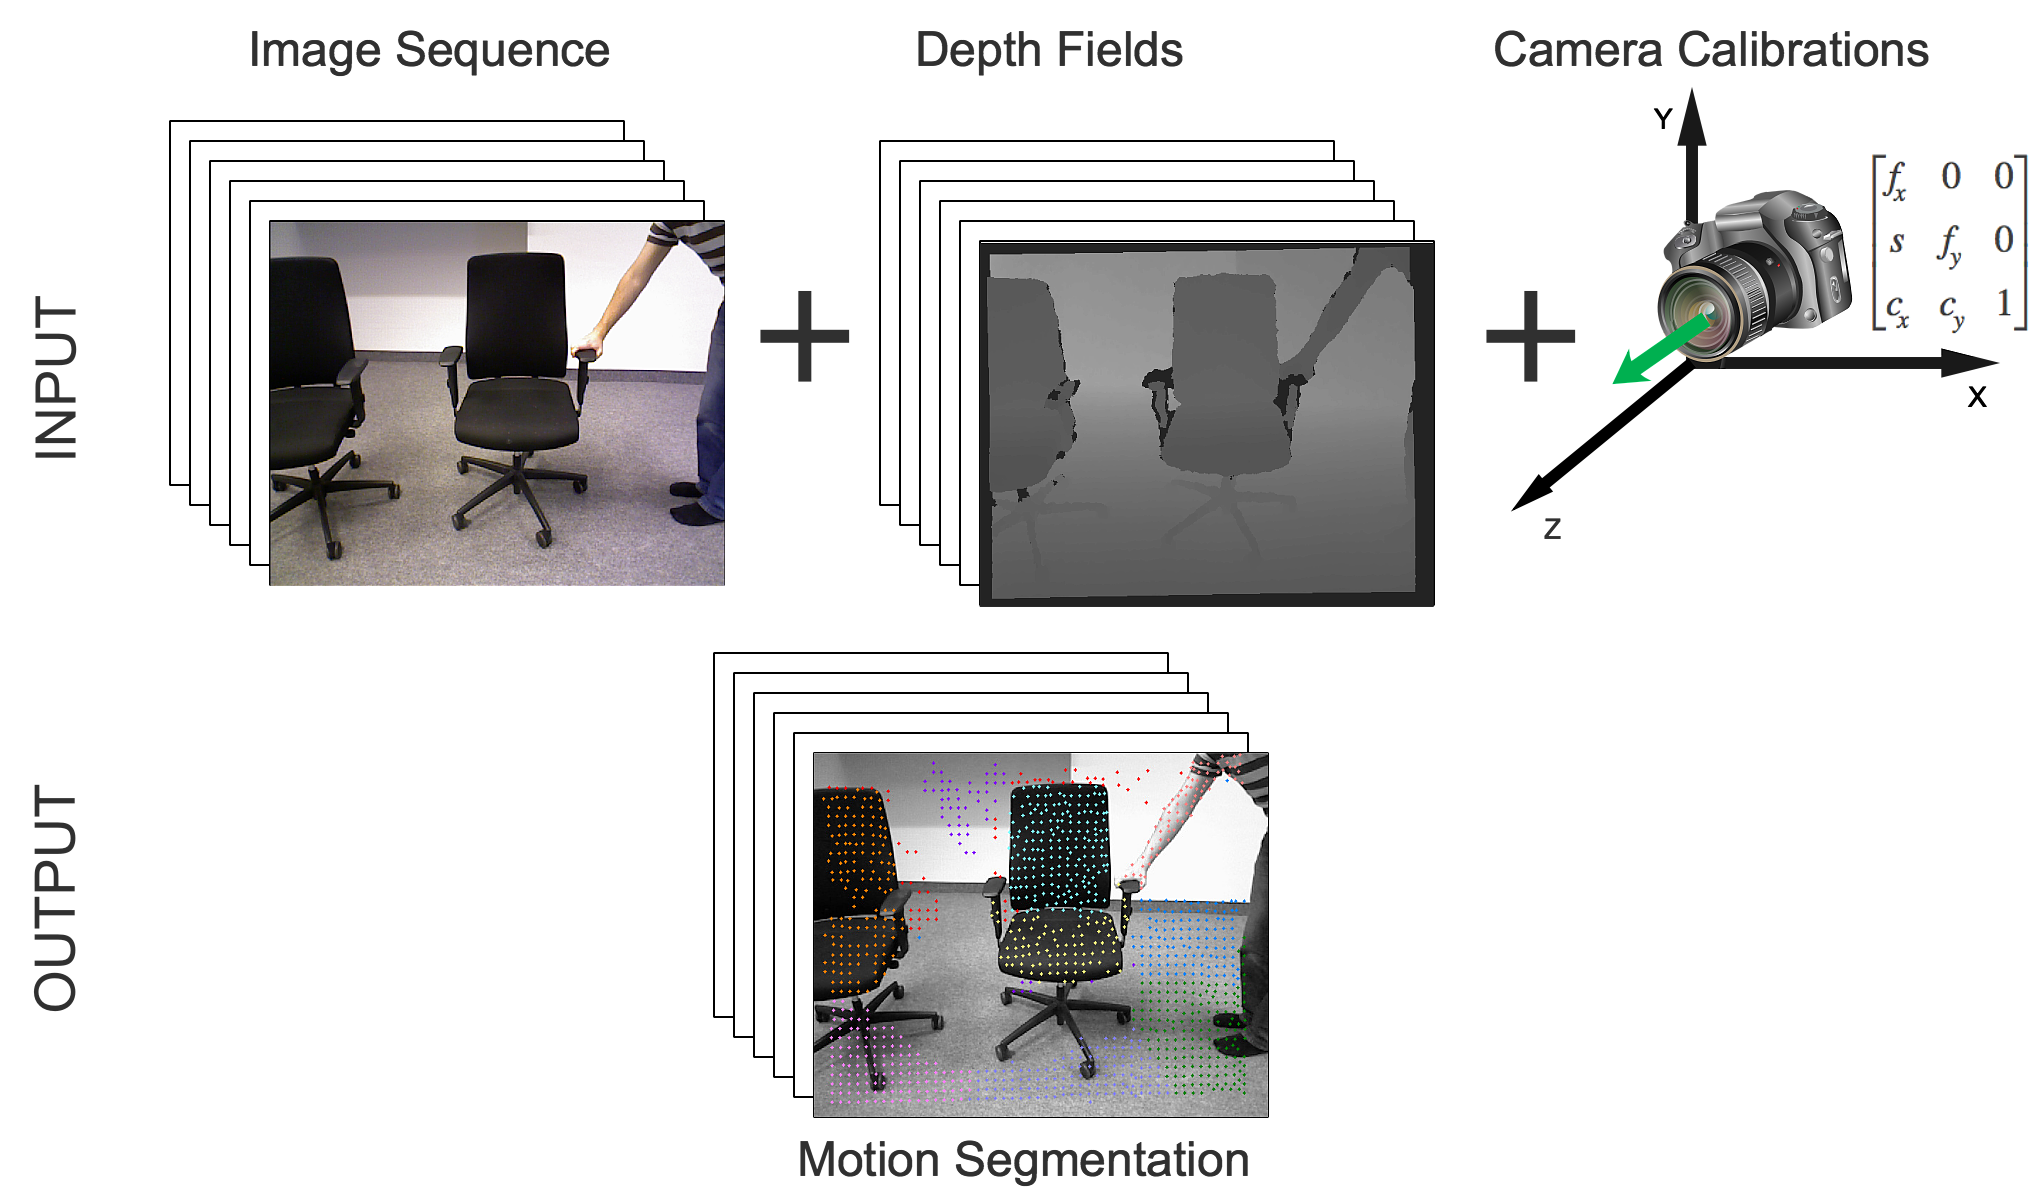
\includegraphics[width=1\linewidth] {introduction/problem_statement_ref}
\end{center}
\caption[Problem Statement]{ foobar }
\label{fig:problem_statement}
\end{figure}



\begin{itemize}
  \item supports a moving camera
  \item be able to deal with occlusions
  \item can handle multiple objects
  \item is robust to nois
  \item can process a coherent sequence of images (video)
  \item can deal with missing data
\end{itemize}

assumptions: only handles rigid motion
 
In addition, this thesis evaluates different flow-and segmentation methods and discusses their shortcomings.

List of main contribution

\begin{itemize}
  \item Give an introduction into the field of optical flow, motion segmentation and clustering algorithms.
  \item implement a pipeline that can perform the task of motion segmentation using various visual cues.
  \item evaluate and compare the different approaches and find their drawbacks and benefits.
  \item Use the acquired knowledge and tweak the pipeline.
\end{itemize}


clearly formulate the problem statement
clearly formulate all assumptions

\section{Related Work}

\subsection{Optical Flow}
list various existing methods to compute the optical flow

a vector motion field which describes the distribution of the apparent velocities of brightness patterns in a sequence. 

first formalized and computed  for  image  sequences  by  Horn  and  Schunck $\cite{HS}$ in  the  1980. Since the pioneering work of Horn and Schunck, many other approaches have been proposed:

\subsection{Motion Segmentation}
In this section we describe different approaches that can be used to address the task of motion segmentation.

\paragraph{Image Difference:} Taking the difference between two frames is a simple technique for detecting changes. By thresholding the intensity difference of two frames, a coarse map of the temporal changes can be obtained. Despite its simplicity, this techniques is limited by the presence of noise, camera movement (everything is changing) and low frame rates (nothing is changing). However, instead of directly using the difference image as the segmentation, the rough map of the changing areas can be used as a guide to extract spatial or temporal information in order to track the regions. Image difference techniques have been used in the work of $\cite{Cav05}$, $\cite{Li07}$ and $\cite{Col07}$.

\paragraph{Statistical Approach} Motion segmentation can be related to a classification problem, identifying whether a particular pixel belongs to either the background or the foreground. In $\cite{Cre05}$ the authors present a variational approach for segmenting an image into a set of regions of parametric motions using a model based on a conditional probability for the spatio-temporal image gradient. By exploiting Bayesian theory, they derive a cost functional which depends on parametric motion models for each  of a set of regions and on the boundary separating these regions.

\paragraph{Wavelets}
The idea is to exploit the ability of wavelets to perform analysis of the different frequency components of the images and then study each component with a resolution matched to its scale. Usually wavelet multi-scale decomposition is used in order to reduce the noise and in conjunction with other approaches, such as optical flow.

\paragraph{Layer Based} The key idea of layers based techniques is to understand which are the different depth layers in the image and which objects lie on which layer. 

\paragraph{Factorization Methods} Allow to recover the structure and motion by using traced features over a the whole image sequence.

\paragraph{Optical Flow}
track features using the optical flow over the given image sequence, compute affinity matrix based on similarity between the overlapping trajectories, use affinity matrix as an input to solve the segmentation task. LIST work but only shallow and briefly

$\cite{Bro11a}$

\section{Thesis Structure}

The reminder of this thesis is organized as follows:
In chapter 2 we start by providing the reader the relevant background in order to following the later chapters of this thesis. This chapter gives a detailed introduction to the concept of optical flow, to segmentation, spectral clustering and graph cut. It also explains how motion segmentation using optical flow is usually approached. \\ \\
In chapter 3 we develope all relevant derivations used to implemented the final pipeline. \\ \\
In chapter 4 we describe the implementation of our motion segmentation pipeline and all its stages in detail. \\ \\
In chapter 5 we list and discuss the results of some performed experiments. We start by introducing the reader to our used datasets. In our experiments section, we perform a qualitative-, as well as a quantitative evaluation. We explore the impact of the huge parameter-space due to the various stages of the implemented pipeline. Last, we also show some good segmentations, using the best (greedy found) parameters on our datasets. \\ \\
And finally Chapter 6 contains the conclusion of this thesis discussing what has been achieved in this thesis and the drawbacks of the proposed method. It also contains a note about some of my personal experiences during this thesis. 
\newpage{\pagestyle{empty} \cleardoublepage}

\chapter{Theoretical Background}
In this chapter we give a introduction in various topics and areas which are necessary in order to understand the implementation of our pipeline and how its generated results were computed. 

\section{Optical Flow}
\label{sec:optical_flow}
In this section we explain the principles and the idea behind the optical flow. We emphasize this concept by giving an in intuitive definition, followed by a mathematical definition. Next, we discuss how such flow fields can be visualized. Lastly, we summarize and explain the pioneering formulation of HS used to estimate flow fields.

\subsection{Definition}

The optical flow is a visual phenomenon that describes the perception of motion.
By definition, it is the apparent visual motion a moving viewer experiences.

To To give the reader a better, more intuitive understanding of this concept, have a look at figure $\ref{fig:motion_eg}$.
\begin{figure}[H]
\begin{center}
\subfigure[1st Frame]{
   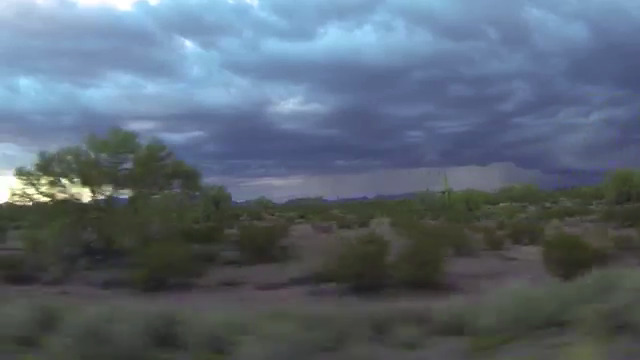
\includegraphics[width=0.47\linewidth] {background/of/ls1}
   \label{fig:motion_eg_f1}
}
\subfigure[2nd Frame]{
   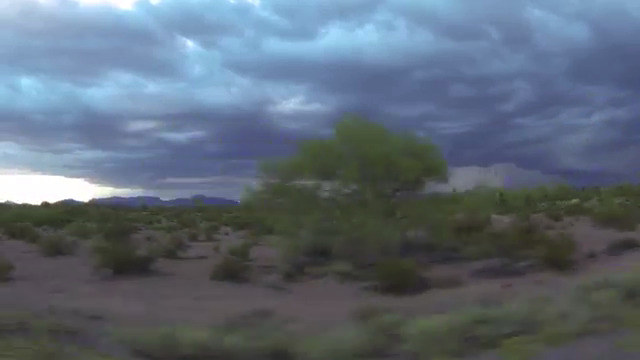
\includegraphics[width=0.47\linewidth] {background/of/ls2}
   \label{fig:motion_eg_f2}
}
~
\subfigure[3rd Frame]{
   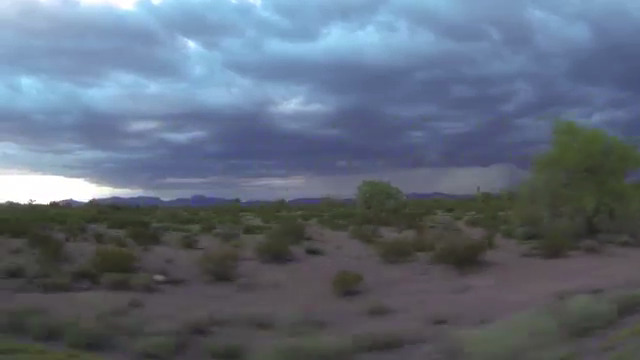
\includegraphics[width=0.47\linewidth] {background/of/ls3}
   \label{fig:motion_eg_f3}
}
\subfigure[4th Frame]{
   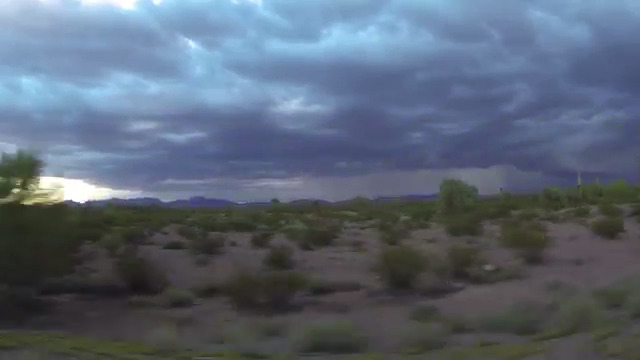
\includegraphics[width=0.47\linewidth] {background/of/ls4}
   \label{fig:motion_eg_f4}
}
\end{center}
\caption[Motion Example]{An example$\footnotemark$ of motion effects illustrated by four frames of a video sequence. Objects far away in the background, such as the mountain or the clouds seems to stand still. Objects being a fair distant apart, but also not too far away can be seen over several frames, such as the tree, that is passed. In addition, we also see observe, that the tree moves along the opposite direction as the driving car. Last, we also see the effect of motion blur for objects that are very close such as the grass.}
\label{fig:motion_eg}
\end{figure}
\footnotetext{The shown frames have been extracted from the following youtube video: \\ \url{https://www.youtube.com/watch?v=lo-pWLmMagc}}
Imagine you sit in a moving car and you are looking out of its windows. While doing so, you will observe that every overtaken object appear to move backwards. Furthermore, objects far in the background seem to stand still, whereas object close to the train seem to move very fast and thus have a blurry look. Therefore, the optical flow is an indicator for distance and size of an object. Moreover, the angle between the observer's viewing direction and the direction of the moving influences the optical flow. if an object travels perpendicular to the train or is directly above or below the it, then the optical flow is maximal. Lastly, an objects directly in front of a viewer will not exhibit any optical flow and thus appear to stand still. However, since not the whole object silhouette is directly in front of the viewer, its edges appear to move and therefore, the such an object appears to get either get larger or smaller, depending on its moving direction.

In summary, the optical flow has the following key properties:
\begin{itemize}
  \item Overtaken objects appear to move backwards.
  \item Distant objects seem to move very slowly and close objects appear to move fast.
  \item The magnitude of the optical flow is doubles if either the speed of the traveling viewer is doubled or the distance to the observed object is halved.
  \item The optical flow varies depending on the angle between the viewing direction and and the direction of movement of the observed object.
  \item The optical flow is maximal if either the object is moving orthogonally towards the viewer's direction or it is moving directly above or below it.
  \item Objects directly in front of a viewer exhibit no optical flow.
\end{itemize}

The underlying basis input of our whole approach depicts the optical flow, computed from a given inputs sequence.

%TODO: Write mathematical definition of the optical flow
\subsection{Mathematical Formulation}


The optical flow is a vector field that defines a point-to-point correspondence between two successive frames. Each vector acts as the displacement of a point in the first frame to match its corresponding point in the second frame.
\subsection{Visualization of Flowfields}

For visualizing flow fields we use the color encoding shown in subfigure $\ref{fig:color_encoding_flows_a}$. The shown color plate provides color values for the normalized flow vectors. The angle in the circle corresponds to the direction and the distance to the center to the velocity. \\ \\
Figure $\ref{fig:color_encoding_flows}$ also contains an example of a flow visualization using these color codes.
\begin{figure}[H]
\begin{center}
\subfigure[Flow Color Codes]{
   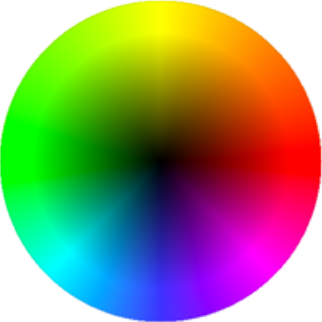
\includegraphics[width=0.35\linewidth] {background/of/flowfield_color_encoding}
   \label{fig:color_encoding_flows_a}
}
~
\subfigure[Example flow visualization]{
   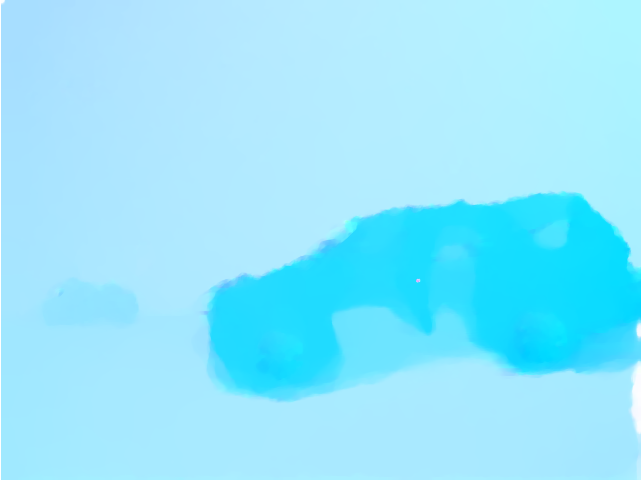
\includegraphics[width=0.5\linewidth] {background/of/cars_fwf_1}
   \label{fig:color_encoding_flows_b}
}
\end{center}
\caption[Visual Color Encoding of Flow Fields]{On the left a visualization of the color plate used to draw flow fields and on the right flow field visualized by this color scheme.}
\label{fig:color_encoding_flows}
\end{figure}

\subsection{Original Flow Estimation Method of H.S.}
\label{sec:hs_formulation}
In the pioneering work of $\cite{Hs81}$ B. Horn and B. Schnunck describe a technique to estimate the optical flow. Back then they defined the optical flow as the distribution of apparent velocities of movement of brightness patterns in an image. \\ \\
Moreover, they already understood the potential of the optical flow and stated the following properties: Can arise from relative motion of objects and the viewer and provide information about the spatial arrangement of the viewed objects and the rate of change in that arrangement. Discontinuities in the optical flow can help to perform segmentation tasks. \\ \\
Sticking to their flow definition they derived an equation that relates the change in the image brightness at a point to the motion of the brightness. \\ \\
Their formulation is based on the following assumptions:
\begin{itemize}
  \item The surface is assumed to be flat. This avoids brightness variations due to shading effects.
  \item The incident illumination is uniform across the surface. Then, the brightness at a point in the image is proportional to the reflectance of the surface at the corresponding point on the object.
  \item The Reflectance varies smoothly and has no spatial discontinuities. Having no discontinuities assures that the image brightness is differentiable.
  \item Situations where objects occlude one another are excluded.
\end{itemize}
These assumptions allow to conclude, that in their model the brightness of a particular point in the pattern is constant. \\ \\
Let the image brightness at a point $(x,y)$ in the image plane at time $t$ be denoted by $E(x,y,t)$. Since the brightness of any point is constant, $\frac{d E}{dt} = 0$ hold true. Using the chain rule for differentiation, they derived the expression in equation $\ref{eq:flow_eq}$.  
\begin{equation}
\begin{aligned}
0 &= \frac{d E}{dt} \\
&= \frac{\partial E}{\partial x} \frac{x}{dt} + \frac{\partial E}{\partial y} \frac{y}{dt} + \frac{\partial E}{\partial t} \\
&= E_{x} u + E_{y} v + E_{t}
\end{aligned}
\label{eq:flow_eq}	
\end{equation}
where we the following substitutions were used to derive the last identity of equation $\ref{eq:flow_eq}$:
\begin{equation}
\begin{aligned}
	u = \frac{dx}{dt} \text{ and } v = \frac{dy}{dt}
\end{aligned}
\end{equation}
By re-ordering the terms of equation $\ref{eq:flow_eq}$ the same way like it has been done in equation $\ref{eq:reordered_flow_eq}$:
\begin{equation}
\begin{aligned}
	(E_x, E_y) \cdot (u, v) &= -E_t \\
	\underbrace{-\frac{1}{E_t}\left( E_x, E_y \right)}_\text{known} \cdot \underbrace{(u, v)}_\text{unknown} &= 1
\end{aligned}
\label{eq:reordered_flow_eq}
\end{equation}
Hence, they could show that the change in image brightness can be formulated by a single linear equations with two unknowns $u$ and $v$, the so called $\textit{flow velocity}$. As a consequence, such a flow velocity cannot be computed locally without introducing additional constraints.




\section{Motion Segmentation}
motion segmentation aims at decomposing a video in moving objects and background by segmenting the objects that undergo different motion patterns.

In this section we describe a conceptual approach how the motion segmentation task using optical flows is commonly approached in literature. 

\subsection{Spectral Clustering}
\subsection{Graph Cut}

multi-label CRF on superpixels for class segmentation $\cite{Fulkerson2009}$

\subsection{Kernighan-Lin Heuristic}


$\cite{Ker70}$

%TODO: maybe we should introduce a section called filtering, containing bilateral filtering, harris corner detector and so forth..
\section{Harris Corner Detector}
\label{sec:harris_corner_detector}

% TODO state idea of an edge

Let us consider a grayscale image $I$. We are going to sweep a window $w(x,y)$ (with displacements u in the x direction and v in the right direction) I and will calculate the variation of intensity. Since we are looking for windows with corners, we are looking for windows with a large variation in intensity. Hence, we have to maximize the equation above, specifically the term:
\begin{equation}
	E \left( u, v \right) = \sum_{x,y} w \left( x,y \right) \left[ I(x + u, y + v) - I(x, y) \right]^2
\label{eq:var_intensitiy_def}
\end{equation}
Next, the term $I(x + u, y + v)$ is expressed by the first order taylor series expansion as the follows:
\begin{equation}
	I(x + u, y + v) = I(x,y) + u I_x (x, y) + v I_y (x,y) + \text{h.o.t}
\label{eq:taylor_exp_intensity}
\end{equation}
Next, we put the first order approximation of equation $\ref{eq:taylor_exp_intensity}$ into equation $\ref{eq:var_intensitiy_def}$ to simplify the definition of $E$.
\begin{equation}
\begin{aligned}
E \left( u, v \right) 
&= \sum_{x,y} w \left( x,y \right) \left[ I(x + u, y + v) - I(x, y) \right]^2 \\
&\approx \sum_{x,y} w \left( x,y \right) \left[ I(x,y) + u I_x (x, y) + v I_y (x,y) - I(x, y) \right]^2 \\
&= \sum_{x,y} w \left( x,y \right) \left[ u I_x (x, y) + v I_y (x,y) \right]^2 \\
&= \sum_{x,y} w \left( x,y \right) u^2 I_x^2 + 2 u v I_x I_y v^2 I_y^2 \\
&= \left( u,v \right) \left( \sum_{x,y} w (x,y)
\begin{pmatrix}
I_x^2 & I_x I_y \\
I_x I_y & I_y^2 \\
\end{pmatrix}
\right) \colvec{u}{v}
\end{aligned}
\label{eq:var_intensitiy_developed}
\end{equation}
Let us define the following substitution
\begin{equation}
M = \sum_{x,y} w  (x,y)
\begin{pmatrix}
I_x^2 & I_x I_y \\
I_y^2 & I_x I_y \\
\end{pmatrix}
\label{eq:var_intensity_sub}
\end{equation}
Putting the substitution from equation $\ref{eq:var_intensity_sub}$ into the final form of equation $\ref{eq:var_intensitiy_developed}$ we obtain the final form
\begin{equation}
	E \left( u, v \right) \approx \left( u,v \right) M \colvec{u}{v}
\end{equation}.
A score is calculated for each window, to determine if it can possibly contain a corner:
\begin{equation}
\begin{aligned}
& R = \det(M) - \kappa \left(\text{trace}(M)\right)^2 \\
&\text{where } \det(M) = \lambda_1 \lambda_2 \text{ and } \text{trace}(M) = \lambda_1 + \lambda_2
\end{aligned}
\label{eq:harris_response}
\end{equation}

\section{Camera Calibrations}






\newpage{\pagestyle{empty} \cleardoublepage}

\chapter{Derivations}
In this section we derive all necessary expressions that are required in order to implement a motion segmentation pipeline described in the next chapter.
% TODO: explain how depths are aligned to color images.
% TODO explain how tracking candidates are computed

\section{Motion Segmentation Pipeline}

\section{Trajectory Affinities}
\label{sec:trajectory_affinities}
In this section we explain how we calculate similarities between extracted trajectories. This computation is the fundamental step of our work.
Before going into details, let us first revisit the definition of a trajectory. By the term trajectory we refer to a list of tracking points, which is ordered by the frame index in which each point was traced. Therefore, every points knows to which frame it belongs to. \\ \\
Let $A$, $B$ denote two trajectories resulting from the previous tracking step. Our goal is to define the similarity between the trajectories by computing a distance $d(A,B)$ between every trajectory pair. For that purpose we exploit their maximal dissimilarity via their maximal motion difference among all frames of common visibility. The squared version of this conceptual formula description is listed in equation $\ref{eq:prod_dist_affinity}$ 
\begin{equation}
	d^2 \left( A, B \right) = \max_t d_t^2 \left( A, B \right)
	\label{eq:product_distance}
\end{equation}
The resulting distance value from equation $\ref{eq:product_distance}$ is then turned into a affinity via the transformation
\begin{equation}
	w \left( A, B \right) = e^{ -\lambda d^2 (A, B) }.
	\label{eq:prod_dist_affinity}
\end{equation}
This measure is based on the work of Shepard $\cite{Shepard87}$ who proposed as a universal law that distance and perceived similarity are related via an exponential function.


where

\begin{equation}
	d_t^2 \left( A, B \right) = d_{spatial}^{A,B} \left( d_{motion}^{A,B} (t) \right) ^2
\end{equation}

\begin{equation}
	d_{spatial}^{A,B} = \frac{1}{\omega - \alpha + 1} \sum_{k=\alpha}^\omega \norm{A(k) - B(k)}
\label{eq:spatial_distance}	
\end{equation}
where $\alpha$ is the first- and $\omega$ is the last- overlapping frame index between the two given trajectories $A$ and $B$.

\begin{equation}
	d_{motion}^{A,B} \left( t \right)  = \frac{\norm{\partial_t A - \partial_t B}}{\sigma_t}
\label{eq:motion_distance}
\end{equation}
The expression $\partial_t A$ denotes the averaged motion over time, which is computed by approximating the derivatives $\partial_t A$, $\partial_t B$ using forward differences with a certain timestep $T$.

\begin{equation}
	\partial_t A = \frac{1}{T} \left( x_{t+T}^{A} - x_{t}^{A}, y_{t+T}^{A} - y_{t}^{A}\right)
\end{equation}
The exact value of $T$ is either the number of overlapping frames between the $A$ and $B$ or a fixed number, in case there are fewer common frames available, than a fixed threshold. \\ \\
Please note that by computing the affinity for every existing trajectory pair combinations, as defined in equation $\ref{eq:prod_dist_affinity}$, we implicitly encode a $n \times n$ affinity matrix $W$, for $n$ given trajectories. 

\section{Eigendecomposition of Graph Laplacians}
Given the pairwise affinity matrix $W$ as computed in section $\ref{sec:trajectory_affinities}$ on page $\pageref{sec:trajectory_affinities}$. An example of such an matrix is shown in figure $\ref{fig:cars_affinity_mat_sub}$. An approximated partitioning of the underlying graph can be obtained by running a variant of spectral clustering. Let
\begin{equation}
	D = \text{diag} \left( d_{A_1}, \dots, d_{A_n} \right)
\label{eq:def_d_mat}
\end{equation}
be the $n \times n$ diagonal matrix with the entries
\begin{equation}
	d_{A_k} = \sum_B w \left( A_k, B \right)
\end{equation}
The eigendecomposition of the normalized graph Laplacian is given by equation $\ref{eq:normalized_graph_laplacian}$.
\begin{equation}
	V^{T} \Lambda V = D^{-\frac{1}{2}} \left( D - W \right) D^{-\frac{1}{2}}
	\label{eq:normalized_graph_laplacian}
\end{equation}
Where $V$ denotes a matrix containing the column-wise eigenvectors of the Laplacian and $\lambda$ is a diagonal matrix containing the corresponding eigenvalues. Figure $\ref{fig:cars_eigenvectors_laplacian}$ shows two example eigenvectors, resulting from the $\textit{cars}$ dataset.

\begin{figure}[H]
\begin{center}
\subfigure[Eigenvector Front-Car]{
   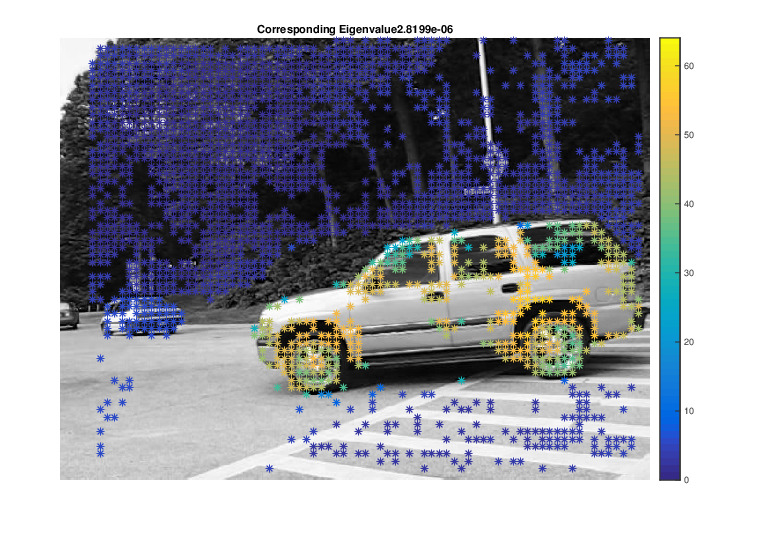
\includegraphics[width=0.48\linewidth] {derivation/eigenvectors/cars/ev_cf}
   \label{fig:cars_eigenvectors_laplacian_a}
}
\subfigure[Eigenvector Back-Car]{
   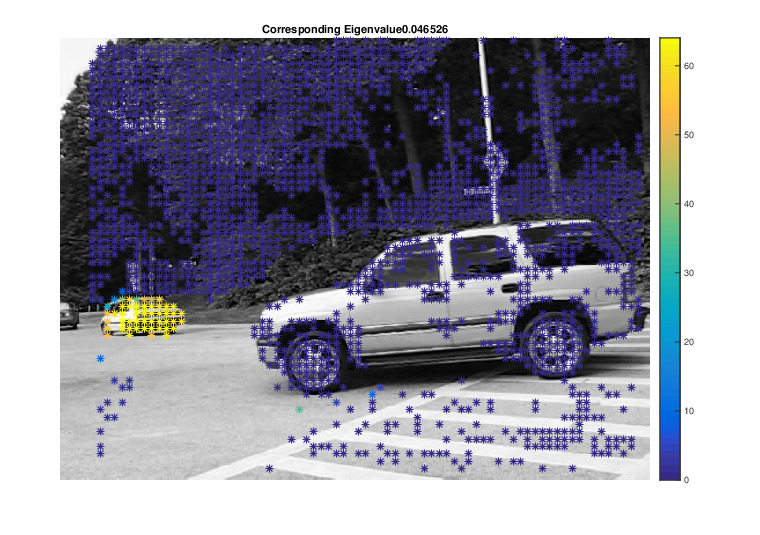
\includegraphics[width=0.48\linewidth] {derivation/eigenvectors/cars/ev_cb}
   \label{fig:cars_eigenvectors_laplacian_b}
}
\end{center}
\caption[Eigenvectors of the Laplacian]{Visualizing the contribution of two significant eigenvectors of the Laplacian of the affinity matrix that belong to the \textit{cars} dataset.}
\label{fig:cars_eigenvectors_laplacian}
\end{figure}

\begin{figure}[H]
\begin{center}
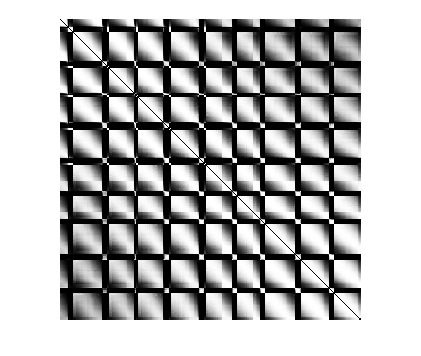
\includegraphics[width=0.7\linewidth] {derivation/eigenvectors/cars/w_mat}

\end{center}
\caption[Affinity Matrix W]{Visualization of the affinity matrix $W$ that belongs to the \textit{cars} dataset.}
\label{fig:cars_affinity_mat_sub}
\end{figure}
To obtain a simple segementation, we could run k-means on the first $k$ eigenvectors, that belong to the smallest k-eigenvalues. This approach yields a one-to-one mapping between cluster assignments and trajectory labels. However, the eigenvectors are often not piece-wise constant. Therefore, running k-means directly on the eigenvectors is not the best choice, since then the eigenvectors get approximated by multiple constant functions and thus the clustering yields an oversegementation. \\ \\
To address this issue we instead formulate a certain energy, containing a spacial regularity term that does not prefer spacial compact clusters. Moreover, it also takes edges in the eigenvectors into account. \\ \\
Let $v_i^A$ denote the $A-th$ component of the $i-th$ eigenvector in $V$ and $\bf{v}^A$ the vector composed of the $A-th$ components of the $m$ eigenvectors. Moreover, let $\mathcal{N}(A)$ denote the set of neighboring trajectories based on the spacial average distance. Then, we want to find the optimal cluster assignments $\pi^A \in {1, \dots, K}$ for a fixed, given number of clusters $K$, such that energy in equation $\ref{eq:min_cut_energy}$ gets minimized.	
\begin{equation}
\begin{aligned}
& E \left( \pi, K \right) = \sum_{A} \sum_{k=1}^K \delta_{\pi^A, k} \norm{\bf{v}^A - \mu_k}_{\lambda} + \nu \sum_A \sum_{B \in \mathcal{N}(A)} \frac{1- \delta_{\pi^A, \pi^B}}{\norm{\bf{v}^A - \bf{v}^B}} \\
& \text{where } \norm{\bf{v}^A - \bf{\mu}}_\lambda = \sum \frac{v_i^A -  \mu_i}{\lambda_i}
\end{aligned} 
\label{eq:min_cut_energy}
\end{equation}
The expression $\mu_k$ denotes the centroid of cluster $k$.

% TODO: explain the terms in the sum


\section{Minimum Cost Multicut Problem}



The min. cost multicut problem is the problem of decomposing a graph $G = (V, E)$ into an optimal number of segments such that the overall cost in term of of edge weights $c_e$ is minimized. The node labeling problem can equivalently be formulated as a binary edge labeling problem
\begin{equation}
\begin{aligned}
& \min_{y \in \{0,1 \}^{|E|}} \sum_{e \in E} c_e y_e \\
& \text{subject to } y \in MC
\end{aligned}
\end{equation}
where $MC$ is the set of all characteristic functions of all multicuts. This corresponds to all $y \in \{0,1 \}^{|E|}$ that form a closed boundaries, representing a valid decomposition of the graph. \\ \\
A formal decomposition of these characteristic functions can be described as the follows:
\begin{equation}
	\forall C \in \text{cycles}(G) \forall e \in C: y_e \leq \sum_{e^{'} \in C \backslash \{e\}} y_{e^{'}}
\end{equation}
It was shown, that is is sufficient to consider all chordless cycles, i.e. all cycles in which each node is only connected to its successor and predecessor. To avoid trivial solutions, the edge weights are typically chosen to be negative for edges that should be cut and positive for those connection nodes that should be joined. \\ \\
Given the cut probabilities $p_e$ of an edge $e \in E$, the negative of the \textit{logit} function 
\begin{equation}
	\text{logit}\left( p_e \right) = \log \left( \frac{p_e}{1 - p_e} \right)
	\label{eq:logit_function}
\end{equation}
provides such a behavior. A plot if the negative logit function defined as in $\ref{eq:logit_function}$ is shown in figure $\ref{fig:negative_logit_function}$.
\begin{figure}
\centering
\begin{tikzpicture}[trim axis left]
\begin{axis}[
  axis x line=center,
  axis y line=center,
  grid=both,
  xtick={-2,-1,...,1,2},
  ytick={-2,-1,...,1,2},
  xlabel={$x$},
  ylabel={$-\text{logit}\left( x \right)$},
  xlabel style={below right},
  ylabel style={above left},
  no markers,
  xmin=-0.5,
  xmax=1.5,
  ymin=-1.5,
  ymax=1.5]
\addplot +[thick, domain=0:1] {-log10(x/(1-x)};
\end{axis}
\end{tikzpicture}
\caption[Logit Function Plot]{A plot of the negative logit function applied on the domain [0,1].}
\label{fig:negative_logit_function}
\end{figure}
If $p_e < 0.5$ then $\text{logit}\left( p_e \right) > 0$ and thus the according edge cost $c_e$ is positive and therefore the edge $e$ is expensive to be cut out from the graph. Conversely, in case that $p_e > 0.5$ the negative logit function of $p_e$ is smaller than zero and thus it is beneficial to cut e. \\ \\
For computing pseudo-probabilities, we use the inverse of the logit function, the so called logistic function
\begin{equation}
	f(z) = \frac{1}{1 + \exp \left( -z \right)}.
	\label{eq:logistic_function}
\end{equation}
The input values we put into the function from equation $\ref{eq:logistic_function}$ are computed by the transformed trajectory distances $d$:
\begin{equation}
	z \equiv z(d) = \beta_0 + \beta_1 d
\end{equation}
The prior probability of cutting two trajectories is defined by the intercept value $\beta_0$. Assuming we learned $\beta_0$ for a certain prior cut probability $p$ and are given a new prior cut probability $\tilde{p}$, we can adapt the value $z$ by
\begin{equation}
	z = \beta_0 - \log \left( \frac{p}{1-p} \right) + \log \left( \frac{\tilde{p}}{1-\tilde{p}} \right) + \beta_1 d.
\end{equation}
If the cut prior is increased, more edges will be cut and the number of resulting segments increases. Small cut priors results in an undersegmentation. \\ \\
In the following we define a measure for the trajectory distances. This distances makes use of the motion-, spatial- and color distance of the overlapping segments between two trajectories $A$ and $B$. Note that the definition of the motion distance is given by equation $\ref{eq:motion_distance}$ and the spatial distance is given by the definition stated in equation $\ref{eq:spatial_distance}$. For the color distance we compute the average color within the overlapping frames using the CieLab\footnote{The key property of the Cie Lab color space is that its values are uniformly spaced. This allows us to use the l2 norm in order to compute meaningful color differences.} color space. More precisely, the color distances $d_{color}$ is defined as the follows:

\begin{equation}
	d_{color}^{A,B} = \frac{1}{\omega - \alpha + 1} \sum_{k=\alpha}^\omega \norm{\text{ColorAt}(k, A(k)) - \text{ColorAt}(k, B(k))}_2
	\label{eq:color_dist}
\end{equation}
where $ColorAt(k, A(k))$ yields the CieLab color value in frame $k$ at the image location $A(k)$\footnote{Remember that $A(k)$ denotes the tracking position of trajectory $A$ in frame $k$}.
The final trajectory distance is computed by combining the described distance values as in equation $\ref{eq:sum_dist}$.
\begin{equation}
\begin{aligned}
z ( A, B ) = \max (\tilde{\beta_0} & + \beta_1 d_{motion}^{A,B} \\
& + \beta_2 d_{spatial}^{A,B} \\
& + \beta_3 d_{color}^{A,B},\\
\beta_0 & + \beta_1 d_{motion}^{A,B} )
\end{aligned}
\label{eq:sum_dist}
\end{equation}
If the sum of the spatial and the color distance is large in equation $\ref{eq:sum_dist}$ then only the motion distances are considered. This ensures that trajectories which are far apart but move similarly still end up in the same segment.

\section{Hole Filling}
\label{section:hole_filling}
In this section we address the problem of \emph{Hole Filling} by formulating this problem as a convex optimization. This formulation should enable us to generate dense segmentations from sparse segmentations. For solving the problem we develop and apply a primal-dual approximation. 
Given an image $g$ has missing information in form of holes, we want to find an optimal reconstructed image $u$. For describing the optimality property we take into account a cost function that describes the color smoothness and also that the resulting image $u$ should be close to the given raw input image $g$. \\ \\
More precisely, let $g$ denote a color image that exhibits holes. Then we want to solve for $u=(u_r, u_g, u_g)$ (RGB image) by minimzating the following energy term (cost function):
\begin{align}
	E(u_c) = \norm{\nabla u_c}_2 + \frac{\lambda}{2} \norm{u_c - g}^2_{\Omega_{c}}
\label{eq:basis_cost_demosaicing}	
\end{align}
with the measure
\begin{equation}
	\norm{u_C - g}^2_{\Omega_{C}} = \sum_x \sum_y \Omega_{C}(x,y)\norm{u_{c}(x,y) - g(x,y)}^2
\label{eq:measure}
\end{equation}
where C denotes the three different color channels. $\Omega_{C}$ is defined such that $\Omega_{C}(x,y) = 1$ if the pixel value at $(x,y)$ is \emph{valid}$\footnote{this means that the pixel at location (x,y) is valid for the bayer color mask C}$ and $\Omega_{C}(x,y) = 0$ when the data is missing. \\ \\
The cost function from equation $\ref{eq:basis_cost_demosaicing}$ consists of a smoothness term, $\norm{\nabla u_c}_2$ and $\norm{u_c - g}^{2}_{\Omega_{c}}$. The first term ensures a smooth color transition between colors in a l2 norm sense. The second term ensures that the reconstructed images does not deviate too much from the given input, i.e. de demosaiced image should resemble to the provided mosaiced raw camera image. This similarity term is further parameterized by a regularization term $\lambda$, indicating how strong the output should match the given input according to the formulated measure in equation $\ref{eq:measure}$. In summary, larger values for $\lambda$ weight the similarity of the input and output image more, and contrarely, lower values weight the color smoothness term more. \\ \\
Hereby, minimizating the cost function from equation $\ref{eq:basis_cost_demosaicing}$ leads to an optimal demosaiced image $u$.
Mathematically we want to solve for 

\begin{equation}
	\widetilde{u} = \argmin_{u_c} E(u_c)
\label{eq:our_general_cost_function}
\end{equation}
We can further simplify the cost function stated in equation $\ref{eq:basis_cost_demosaicing}$ relying on the following observation: Since the function $\Omega_{C}$ is only true for pixels that correspond to the color channel C in the bayer mask, we see that 
\begin{equation}
	\Omega_{C}(x,y)\norm{u_{c}(x,y) - g(x,y)}
\end{equation}
is only not equal zero if the pixel at location $(x,y)$ belongs to the color channel $C$. Therefore we are allowed to solve the stated optimization problem from equation $\ref{eq:basis_cost_demosaicing}$ for each color channel separately. 


According to this insight we are supposed to minimize the following three independent$\footnote{Independent in the sense that we are allowed to solve for each color channel separately}$ convex problems:



\begin{align}
	\widetilde{u}_R = \argmin_{u_R} \norm{\nabla u_R}_2 + \frac{\lambda}{2} \norm{u_R - g}^2_{\Omega_{R}} \nonumber \\
	\widetilde{u}_G = \argmin_{u_G} \norm{\nabla u_G}_2 + \frac{\lambda}{2} \norm{u_G - g}^2_{\Omega_{G}}\nonumber \\
	\widetilde{u}_B = \argmin_{u_B} \norm{\nabla u_R}_2 + \frac{\lambda}{2} \norm{u_B - g}^2_{\Omega_{B}}
\label{eq:our_convex_probelm}		
\end{align}

Where we still rely on the measure defined in equation $\ref{eq:measure}$ but C was replayed by the appropriate color channel$\footnote{C stands for either the color channel R, G or B.}$. We notice that the equations in $\ref{eq:our_convex_probelm}$ tell us that we have to solve three different energies similar to the one formulated in equation $\ref{eq:our_general_cost_function}$.

In the next section we will describe how to solve the stated minimization problems from equation $\ref{eq:our_convex_probelm}$ numerically.

\subsection{Primal-Dual Form}
In this section we derive the primal-dual form of the stated convex demosaicing problem.

But first off, let us consider an initial problem of the form 

\begin{align}
	\min_{x \in X} F(K x) + G(x)
\label{eq:initial_primal}	
\end{align}

where $F$, $G$ are convex functions and $K$ denotes a linear operator. 

The primal-dual formulation for equation $\ref{eq:initial_primal}$ is given by 

\begin{align}
	\min_{x \in X} \max_{y \in Y} < Kx, y > - F^*(y) + G(x)
\label{eq:initial_primal_dual}	
\end{align}


For a given mosaiced RGB image $u_{RGB}$ encoded as a 3 dimensional $M \times N$ matrix, i.e. a tensor of dimension $M \times N \times 3$. As mentioned in the problem statement we can solve three independent convex problems in order to solve the problem of demosaicing a RGB image. Therefore let in the following $u$ define stand for one particular color channel of the given color image $u_{RGB}$.

\begin{equation}
\min_{u \in U} \norm{\nabla u} + \frac{\lambda}{2} \norm{u - g}^2_{\Omega}
\label{eq:initial_energy}
\end{equation}

where $\norm{u - g}^2_{\Omega}$ is defined as in equation $\ref{eq:measure}$ and $g$ is the corresponding color channel of the mosaiced image described in the problem statement.

We observe that equation $\ref{eq:initial_energy}$ has the same structure as the initial problem stated in equation $\ref{eq:initial_primal}$. This allows us to formulate the primal-dual form of equation $\ref{eq:initial_energy}$ which will look like the following:

\begin{align}
	\min_{u \in U} \max_{y \in Y} < Kx, y > - F^*(y) + G(x)
\label{eq:initial_primal_dual}	
\end{align}

Where $K$, $F$ and $G$ are defined as:

\begin{align}
	K &= \nabla \nonumber \\
	F &= \norm{\cdot}_2 \nonumber \\
	G &= \norm{u - g}^2_{\Omega}
\label{eq:def_kfg}	
\end{align}

Note that $F*$ denotes the convex conjugate form of $F$. The convex conjugate of $F$ has an explicit identity that can be computed using the Legendre-Fenchel-Transform.

\begin{align}
	F^*(y) &= (\norm{\cdot}_2)^*(y) \nonumber \\
		  &= \sup_x x^T y - \twonorm{x} \nonumber \\
		  &= \sup_x x^T y - \max_{\twonorm{z} \leq 1} x^T z \nonumber \\
		  &= \sup_x \min_{\twonorm{z} \leq 1} x^T(y-z) \nonumber \\
		  &= \begin{cases}
   				0  			& \text{if} \twonorm{y} \leq 1 \\
   				\infty      & \text{otherwise}
  			 \end{cases} \nonumber \\
  		  &= \delta(y)
\label{eq:legendre_fenchel_transform_f}  		  
\end{align}

The first equality is simply the definition of $F$. The second equality is using the so called Legendre-Fenchel transformation,

\begin{equation}
	(\norm{\cdot}_2)^*(y) = \sup_x x^T y - \twonorm{x} \nonumber
\end{equation}. 

In the third equality I make use of the Cauchy-Schwarz inequality, 
\begin{equation}
	\twonorm{x} = \max_{\twonorm{z} \leq 1} x^T z
\end{equation}


Plugging equation $\ref{eq:legendre_fenchel_transform_f}$ and the definitions in from equation $\ref{eq:def_kfg}$ into the primal-dual equation equation $\ref{eq:initial_primal_dual}$ we conclude the following final primal-dual formulation:

\begin{equation}
\min_{u \in U} \max_{y \in Y} <\nabla u, y> - \delta(y) + \frac{\lambda}{2}\norm{u - g}^2_{\Omega}
\label{eq:final_primal_dual}
\end{equation}


\subsection{Primal-Dual steps}
In this section I will present an iterative solver for our stated primal-dual formulation.

In the following I am going to rely on an algorithm $\cite{chambolle2011first}$ formulated by A.Chambolle and T.Pocke, which allows to solve primal-formulations as ours stated in equation $\ref{eq:final_primal_dual}$.
They stated an iterative algorithm that has the following update steps:

\begin{align}
	y^{n+1} &= \prox_{\sigma F^*}(y^n + \sigma K \bar{x}^n) \nonumber \\
	x^{n+1} &= \prox_{\tau G}(x^n - \tau K^* y^{n+1}) \\
	\bar{x}^{n+1} &= x^{n+1} + \theta(x^{n+1} - x^n)
\label{eq:update_rules_plain}	
\end{align}
with $\theta \in (0, 1]$ and the constraint $\tau \sigma \norm{K}^2 < 1$. Note that stated constraint is important in order to guarantee convergence of their algorithm.

Hereby $prox(\cdot)$ denotes the proximity operator and is defined as 

\begin{equation}
	\prox_{\lambda F}(z) = \arg \min_x \frac{1}{2} \twonorm{x - z}^2 + \lambda F(x)
\end{equation}

In the following we will derive explicit identities for the update rules in equation $\ref{eq:update_rules_plain}$that can be numerically solved. Our goal is to find an expression for the proximity operator.

\subsection{Update for $y^{n+1}$}

In this subsection we derive an identity for the $y^{n+1}$ update rule from equation $\ref{eq:update_rules_plain}$. The key idea is to use the so called Moreau's Identity:  

\begin{equation}
	\prox_{\lambda F^*}(z) = z - \lambda \cdot \prox_{F/ \lambda}(z / \lambda) 
\label{eq:moreau}	
\end{equation}

Next, we apply the Moreau's identity to the proximity operator of the Legendre-Fenchel transformation.


\begin{align}
	\prox_{\lambda F^*}(y^n + \sigma K \bar{x}^{n}) 
	&= (y^n + \sigma K \bar{x}^{n}) - \sigma \prox_{\frac{F}{\sigma} } \left(\frac{y^n + \sigma K \bar{x}^{n} }{\sigma} \right) \nonumber \\
	&= (y^n + \sigma K \bar{x}^{n}) - \sigma \left( \frac{y^n + \sigma K \bar{x}^{n} }{\sigma} \max{0, 1-\frac{1}{\twonorm{y^n + \sigma K \bar{x}^{n} }}} \right) \nonumber \\
	&= (y^n + \sigma K \bar{x}^{n}) - \left( y^n + \sigma K \bar{x}^{n} \right) \max{\left(0, 1-\frac{1}{\twonorm{y^n + \sigma K \bar{x}^{n} }}\right)}  
\label{eq:y_n_1_expression}
\end{align}

For the first equality we use the definition of equation $\ref{eq:moreau}$ and for the second equality we used the fact (proven during class) that

\begin{align}
	\prox_{\frac{\twonorm{\cdot}}{\sigma}}(\frac{x}{\sigma}) = \frac{x}{\sigma} \max{\left(0, 1-\frac{1}{\twonorm{x}}\right)}
\end{align}

To simplify our derivation even and also get rid of the proximity operator we next make a case distinction for $\twonorm{y^n + \sigma K \bar{x}^{n}}$. 

\begin{itemize}
	\item If $\twonorm{y^n + \sigma K \bar{x}^{n}} \geq 1$
		then  
		\begin{align}
			0 \leq 1-\frac{1}{\twonorm{y^n + \sigma K \bar{x}^{n}}} \leq 1
		\end{align}
		
		Therefore $\frac{1}{\twonorm{y^n + \sigma K \bar{x}^{n}}}$ is smaller than one and thus
		
		\begin{align}
			\max{\left(0, 1-\frac{1}{\twonorm{y^n + \sigma K \bar{x}^{n}}}\right)} 
			&= 1-\frac{1}{\twonorm{y^n + \sigma K \bar{x}^{n}}}
		\end{align}
		
		This insight can directly be used for the maximum expression in equation $\ref{eq:y_n_1_expression}$ and we hence obtain:
		
		\begin{align}
			\prox_{\lambda F^*}(y^n + \sigma K \bar{x}^{n})
			&= (y^n + \sigma K \bar{x}^{n}) - \left( y^n + \sigma K \bar{x}^{n} \right) \max{\left(0, 1-\frac{1}{\twonorm{y^n + \sigma K \bar{x}^{n} }}\right)} \nonumber \\
			&= (y^n + \sigma K \bar{x}^{n}) - \left( y^n + \sigma K \bar{x}^{n} \right) \left( 1-\frac{1}{\twonorm{y^n + \sigma K \bar{x}^{n}}} \right)\nonumber \\
			&= (y^n + \sigma K \bar{x}^{n}) -(y^n + \sigma K \bar{x}^{n}) +\frac{y^n + \sigma K \bar{x}^{n}}{\twonorm{y^n + \sigma K \bar{x}^{n}}} \nonumber \\
			&= \frac{y^n + \sigma K \bar{x}^{n}}{\twonorm{y^n + \sigma K \bar{x}^{n}}}
		\end{align}
		
	\item If $\twonorm{y^n + \sigma K \bar{x}^{n}} < 1$
		then 
		\begin{align}
			1-\frac{1}{\twonorm{y^n + \sigma K \bar{x}^{n}}} < 0
		\end{align}
		thus we conclude 
		\begin{align}
			\max{\left(0, 1-\frac{1}{\twonorm{y^n + \sigma K \bar{x}^{n}}}\right)} 
			&= 0
		\end{align}
		which offers us the following new identity for equation $\ref{eq:y_n_1_expression}$:
		
		\begin{align}
			\prox_{\lambda F^*}(y^n + \sigma K \bar{x}^{n})
			&= (y^n + \sigma K \bar{x}^{n}) - \left( y^n + \sigma K \bar{x}^{n} \right) \max{\left(0, 1-\frac{1}{\twonorm{y^n + \sigma K \bar{x}^{n} }}\right)} \nonumber \\
			&= (y^n + \sigma K \bar{x}^{n}) - \left( y^n + \sigma K \bar{x}^{n} \right) 0 \nonumber \\
			&= y^n + \sigma K \bar{x}^{n}
		\end{align}
\end{itemize}

By using the results from the case distinction from above we can simplify equation $\ref{eq:y_n_1_expression}$ even further to:

\begin{equation}
	\prox_{\lambda F^*}(y^n + \sigma K \bar{x}^{n}) = \frac{y^n + \sigma K \bar{x}^{n}}{\max{\left(1,\twonorm{y^n + \sigma K \bar{x}^{n}} \right)}}
\label{eq:y_p_1_we_proxy}	
\end{equation}

Finally, the only left step to do is to plug in the definition of $K$ into equation $\ref{eq:y_p_1_we_proxy}$ which gives us then the final update rule for $y_{n+1}$ when relying on the update rule from equation $\ref{eq:y_n_1_expression}$:

\begin{align}
	y_{n+1} = \frac{y^n + \sigma \nabla \bar{x}^{n}}{\max{\left(1,\twonorm{y^n + \sigma \nabla \bar{x}^{n}} \right)}}
\label{eq:update_rule_y_n_p_1}	
\end{align} 	

\subsection{Update for $x^{n+1}$}

\begin{align}
x^{n+1} &= \prox_{\tau G}(x^n - \tau K^* y^{n+1}) \\
		&= \prox_{\tau \frac{\lambda}{2} \norm{u - g}_{\Omega}^2 }(x^n - \tau \nabla^* y^{n+1}) \\
	    &= \arg \min_{z} \frac{1}{2} \twonorm{\left(x^n - \tau \nabla^* y^{n+1} \right) - z}^2 + \tau \frac{\lambda}{2}\norm{z - g}_{\Omega}^2 \\
	    &= \arg \min_{z} E(z)
\label{eq:energy_x_p_1}	    
\end{align}

To simplify the following derivations, let us define the following substitution: 
\begin{align}
	m := \left(x^n - \tau \nabla^* y^{n+1} \right)
\end{align}

We can solve for $x^{n+1}$ by finding the zeros of the partial derivative of $E(z)$ from equation $\ref{eq:energy_x_p_1}$. Let us start with the partial derivative along $z$ of $E(z)$ from equation $\ref{eq:energy_x_p_1}$: 

\begin{align}
	\partial_{z} E(z)
	&= \partial_{z} \left( \frac{1}{2} \twonorm{m - z}^2 + \tau \frac{\lambda}{2}\norm{z - g}_{\Omega}^2 \right) \nonumber \\
	&= \frac{1}{2} \partial_{z} \left[ \left( m - z \right)^{T}\left( m - z \right) + \tau \lambda \Omega \left( z -g \right)^{T}\left( z -g \right) \right] \nonumber \\
	&= \frac{1}{2} \partial_{z} \left[ m^{T}m -2m^{T} z + z^{T} z + \tau \lambda \Omega \left( z^{T}z -2z^{T} g + g^{T} g\right) \right] \nonumber \\
	&= \frac{1}{2} \left[ -2m + 2z + \tau \lambda \Omega \left( 2 z -2g \right) \right] \nonumber \\
	&= \left[ -m + z + \tau \lambda \Omega z - \tau \lambda \Omega g \right]	 \nonumber \\	
	&= \left[ \left(1+\tau \lambda \Omega \right)z-m - \tau \lambda \Omega g \right]	 \nonumber \\
\label{eq:derivative_x_n_p_1}		
\end{align}

Next, let us set the finding from equation $\ref{eq:derivative_x_n_p_1}$ to zero and solve for $z$:

\begin{align}
	\partial_{z} E(z) 
	&= 0 \nonumber \\
	&\Leftrightarrow \left(1+\tau \lambda \Omega \right)z-m - \tau \lambda \Omega g = 0 \nonumber \\
	&\Rightarrow z = \left(m +  \tau \lambda \Omega g \right) \left( 1+\tau \lambda \Omega\right)^{-1} \nonumber \\
	&\Rightarrow z = \frac{m +  \tau \lambda \Omega g}{1+\tau \lambda \Omega} \nonumber \\
\label{eq:zeros_ez}	
\end{align}

Note that the division $(1+\tau \lambda \Omega)$ denotes a component-wise division, since $\Omega$ is applied component-wise to the elements of $g$. In addition, 1 and $\Omega$ are representing matrices here (of same dimension as $g$ and $z$ ($u$ respectively).

By plugging the definition $m$ into equation $\ref{eq:zeros_ez}$ and using the fact, that $z$ corresponds to $x^{n+1}$ we can conclude:

\begin{align}
	x^{n+1} 
	&= \frac{x^n - \tau \nabla^* y^{n+1} +  \tau \lambda \Omega g}{1+\tau \lambda \Omega} \nonumber \\
	&= \frac{x^n + \tau div(y^{n+1}) +  \tau \lambda \Omega g}{1+\tau \lambda \Omega}
\label{eq:update_x_n_p_1}	
\end{align}

In the last step we used the well known fact, that 
\begin{align}
	\nabla^* (v) = -div(v)
\end{align}

for any vector-field $v$ of the form 

\begin{align}
	v = \nabla u
\end{align}
 

\newpage{\pagestyle{empty} \cleardoublepage}

\chapter{Implementation}
\newpage{\pagestyle{empty} \cleardoublepage}

% TODO eval all datasets for ldof ped mc, ldof pd sc
%TODO: explain statistical method: precission, recall, f1, density
%TODO: statistics: performance of selected set of methods applied on all datasets: HS_PD_SC, LDOF_PD_SC (classic), LDOF_PED_MC, LDOF_SD, LDOF_SED, SRSF_PED, SRSF_SED
%TODO: statistics: influence of lambda using LDOF_PD
%TODO: statistics: LDOF_PED_SC vs LDOF_PD_SC
%TODO: statistics: LDOF_PED_SC vs LDOF_PED_SC
%TODO: statistics: LDOF_PD_MC vs LDOF_SD
%TODO: statistics: LDOF_PED_MC vs LDOF_SED
%TODO: statistics: best case - tweak paras for a dataset.

%TODO: varying anzahl cluster: chair bonn/cerealbox 2:12, 3d lodf, unmerged results (ped sc, mc, mache plot anz.cluster/f1 score je methode plus prec-recall plot je methode
%TODO: mache overall performance stat. wenn standard params

\chapter{Results}
Finally, in this last section we describe how we evaluate our generated segmentations. Principally, the quality of a resulting segmentation is measured by comparing it against a manually drawn ground truth segmentation image. \\ \\
In the following the term $\textbf{P-affinity}$ refers to an affinity matrix generated by a product distance combination method. That means, that the affinity was produced by either $\textbf{PD}$ or $\textbf{PED}$. Please refer to the section $\ref{sec:affinity_matrix_impl}$ on page $\pageref{sec:affinity_matrix_impl}$ to re-read the definition of these modes. 

\section{Default Parameter Assignments}
\label{sec:spectral_clustering_parameters}
Even though our pipeline mainly consists of tree main components, that is the flow computation stage, the affinity matrix generation stage and the segmentation stage, it exhibits a large amount of parameters that have to be specified. This issues makes it tedious to use our implementation, especially, when running the pipeline repeatedly over and over again (e.g. during our experiments). Therefore, we aim at reducing the number of free parameters in our pipeline by providing certain default assignments. \\ \\
In this section we address this problem of default parameter assignments. In particular we explain which parameter gets what default value assigned to and why. \\ \\
Our motion segmentation pipeline exhibits many parameters since it consists of several stages such as the flow generation- affinity matrix computation- segmentation stage. Moreover, every stage implements different techniques to approach its specified tasks. Hence, a user has to specify both, which pipeline combination should be run and what parameter values of an specific method should be used. To get the overall picture of this complexity we illustrate all available \textit{pipeline combinations} in figure $\ref{fig:pipeline_combinations}$. 
\begin{figure}[H]
\begin{center}

\includegraphics[width=1\linewidth] {evaluation/pipeline_combinations}
\end{center}
\caption[Pipeline Combinations]{A listing of all available pipeline combinations. Our pipeline implements a series of flow methods (4), various affinity computation modes (4) and different segmentation techniques (3). In total, there are $4 \times (2 \times 2 + 2 \times 1) = 24$ different combinations available. However, not every component mode can be combined with any other. For example \textit{S-affinities} can only be used in combination with the \textit{Kernighan-Lin Heuristic} (KL). }
\label{fig:pipeline_combinations}
\end{figure}
In the following we give a brief description of several default assignments used in different pipeline stages. \\ \\
For generating the flow fields we rely on existing implementations as described in section $\ref{sec:generate_of}$. We do not attempt to modify any parameter settings while utilizing those flow methods and thus strictly rely on their default settings. A summary about these flow methods can be found in section $\ref{sec:impl_optical_flow}$ on page $\pageref{sec:impl_optical_flow}$. \\ \\
Before tracking trajectories as described in section $\ref{sec:trajectory_tracking}$, we initially have to extract their feature locations (Sec. $\ref{sec:tracking_candidates}$). The resulting feature extraction is determined by a parameter defining the sparsity of the sampling rate, indicating to use only every $k-th$ feature. Throughout performing our experiments we will be using $k$ equals to 8. This choice is justified by the fact that using a smaller sampling rate would not enhance the result's quality and negatively influence the overall runtime, whereas larger values would cause the opposite. \\ \\
Next some words about choosing defaults for the affinity matrix generation stage. Before computing a $\textit{P-affinity}$, either by running the mode \textit{PD} or $\textit{PED}$, we have to specify a certain value $\lambda$. This parameter is used in equation $\ref{eq:prod_dist_affinity}$ and acts as a scale of the similarity between two trajectories. In the follows we use$\footnote{We determined the defaults by trying out different values for $\lambda$ and took those which yielded the visually most promising results. Please note that this kind of parameter selection is by no means optimal.}$ $\lambda$ equals $0.1$ when running $PD$ and $\lambda = 10$ when running the affinity mode $PED$. The reason for using different $\lambda$ values is because PED and PD have different scales. As we can see $\lambda$ takes different powers to ten. However the exact choice of this scale does not matter$\footnote{Meaning, that it \textit{does not matter} regarding using a different mantissa, since it will not affect the final outcome of the affinity matrix drastically.}$ that much as long as it close to the same power to ten value as its corresponding default. \\ \\
When having a closer look at the computed affinities, we observe, that approximately one third of the trajectory neighbors have similarity large enough to have a big influence on it. Therefore, we decided to set the number of closest neighbors per trajectory equals one third of the total neighbors. An example is shown of such affinities is shown in figure $\ref{fig:cars_w}$. A dark pixel indicates a low affinity between two trajectories and bright regions indicate large affinities. \\ \\
In order to generate S-affinities we rely on the definition of equation $\ref{eq:sum_dist}$, which is used to compute distances between trajectories. However, this equation is parameterized by several weights $\beta$. In this work we use the exactly the same $\beta$ values as defined in the paper $\cite{KB15b}$, which are equal to
\begin{equation}
\begin{aligned}
\bar{\beta}_0 = 6 \text{, } \beta_0 = 2 \text{, } \beta_1 = \beta_3 = -0.02 \text{ and } \beta_2 = -4
\end{aligned}
\end{equation}
In our experiments we set the dummy vertex count in the Kernighan-Lin partitioning method always equals zero. \\ \\
For every segmentation methods, we specified the \textit{cluster count} they are supposed to solve for equals to two times the number of an estimated number of moving objects present in the target dataset. In other words the cluster count $CC$ is an personal estimate and defined as
\begin{equation}
	\text{CC} = 2 \times \text{Estimated Moving Objects in Dataset}
\label{eq:cc_def} 
\end{equation}
This estimation approach only takes into account very clearly, distinct moving objects and is thus probably underestimating the real moving object count. \\ \\
Segmentation methods that rely on P-affinities are utilizing a certain number of eigenvectors resulting from the eigenvalue decomposition of the Laplacian. For this eigenvector Count (EV) we use twice the number of the clusters the methods are supposed to solve for, i.e. this count is defined as
\begin{equation}
	\text{EV} = 2 \times \text{CC}
\end{equation}
Moreover, when using the MC segmentation, we set the default of its data- and smoothness relaxation parameter $\nu$ used by its energy term (defined in equation $\ref{eq:min_cut_energy_revisited}$) equals to the dimension of the affinity matrix times $10^{-6}$. Again, this value has been determined by simply trying out various assignments. Furthermore, we observed that it is sufficient to run about 10-20 iterations until MC converges. Therefore, we conservatively assign the number of iterations $\text{MC}_i$ equals 20. \\ \\
Unless stated otherwise we rely on those parameter default parameter specifications to generate out results. Moreover, in section $\ref{sec:parameter_experiments}$, we offer a statistical justification for the default choices of $\lambda$, $\text{CC}$, $\text{EV}$ and $\text{MC}_i$.

\section{Datasets}
\label{sec:datasets}
In this section we introduce the dataset we were using for generating our results. Our dataset are a diverse collection of videos, originating from various source. Some videos were captures by Microsoft's Kinect, some by Asus' Xtion. Some were manually captures and again others are from other authors. In particular the cars dataset is from the Middlebury dataset$\footnote{See \url{http://vision.middlebury.edu/stereo/data/}}$ and datasets prefixed by \textit{Bonn} are from Bonn's RGB-D Rigid Multi-Body Dataset $\footnote{See \url{http://www.ais.uni-bonn.de/download/rigidmultibody/}}$. \\ \\
We aim to work with a diverse collection of datasets. Meaning that we want to use datasets that capture different types of motions, are recorded in-and outdoor scenes and are captured by a static or moving cameras. Also, our implementation should be able to generated segmentations for long as well as for short sequences. \\ \\
Regularly, a dataset consists of the frames of a RGB-D video and the corresponding depth-and color camera calibrations. Moreover, for a selected set of frames we manually have drawn$\footnote{To draw these ground truth images using Gimp.}$ ground truth (\textbf{GT}) images. Please notice that all GT images were drawn according to the painter's opinion and thus do probably not truly correspond to the real ground truth. \\ \\
In the following a listing of our datasets, listing three of its frames, one of its ground truth motion segmentation images, a list of properties and a brief description what is happening in the video:
\begin{itemize}
\item \textbf{Cars}: \textbf{frames}: 19, \textbf{resolution}: $480 \times 640$, \textbf{depths}: No 
\begin{figure}[H]
\begin{center}
\subfigure[Frame 1]{
   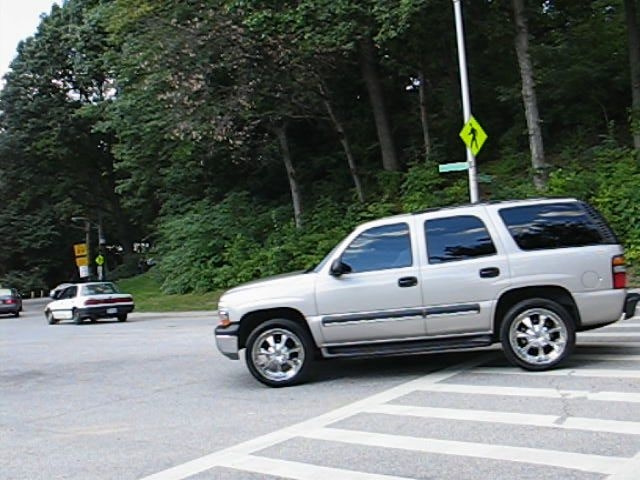
\includegraphics[width=0.22\linewidth] {evaluation/datasets/cars/1}
}
\subfigure[Frame 10]{
   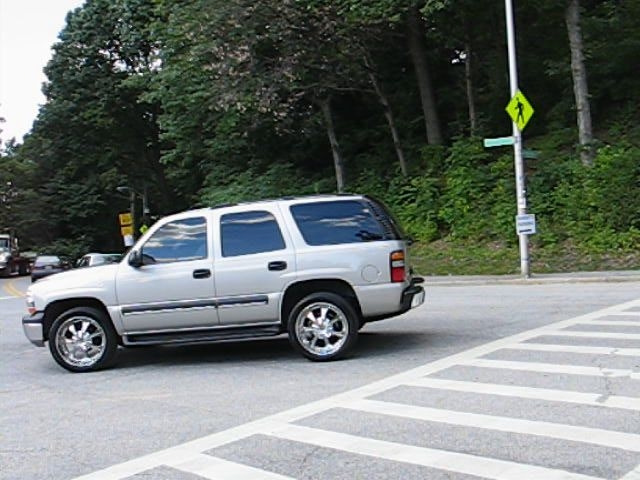
\includegraphics[width=0.22\linewidth] {evaluation/datasets/cars/10}
}
\subfigure[Frame 19]{
   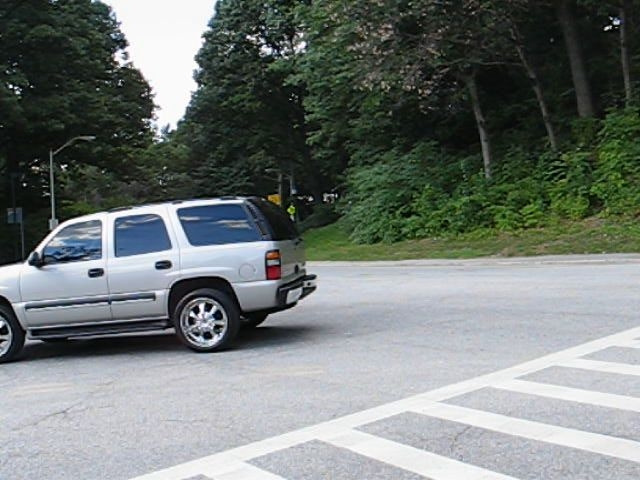
\includegraphics[width=0.22\linewidth] {evaluation/datasets/cars/19}
}
\subfigure[GT Frame 1]{
   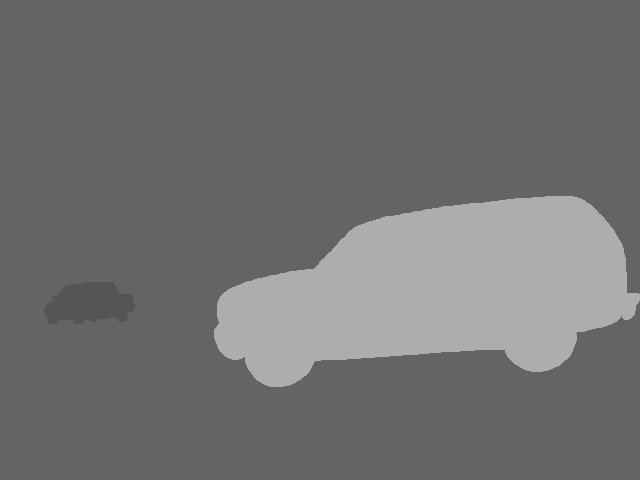
\includegraphics[width=0.22\linewidth] {evaluation/datasets/cars/gt1}
}
\end{center}
\caption[Dataset Bonn Cars]{An outdoor scene showing two cars, both moving to the left. One in the front and the other in the background. The camera is static.}
\label{fig:eval_datasets_cars}
\end{figure}
\item \textbf{Bonn Watercan}: \textbf{frames}: 58, \textbf{resolution}: $480 \times 640$, \textbf{depths}: Yes
\begin{figure}[H]
\begin{center}
\subfigure[Frame 4]{
   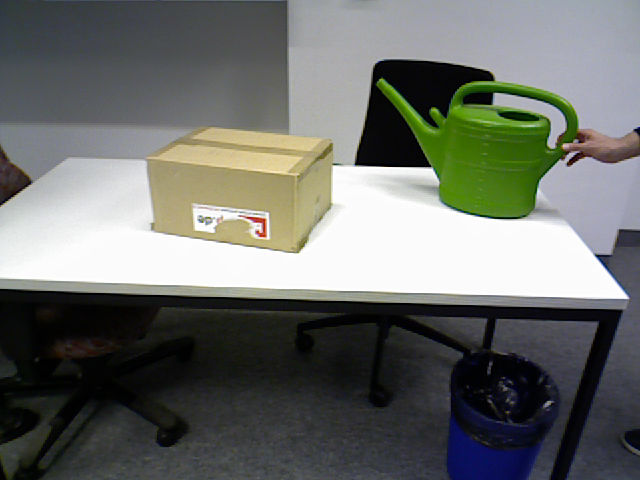
\includegraphics[width=0.22\linewidth] {evaluation/datasets/bonn_watercan/4}
}
\subfigure[Frame 31]{
   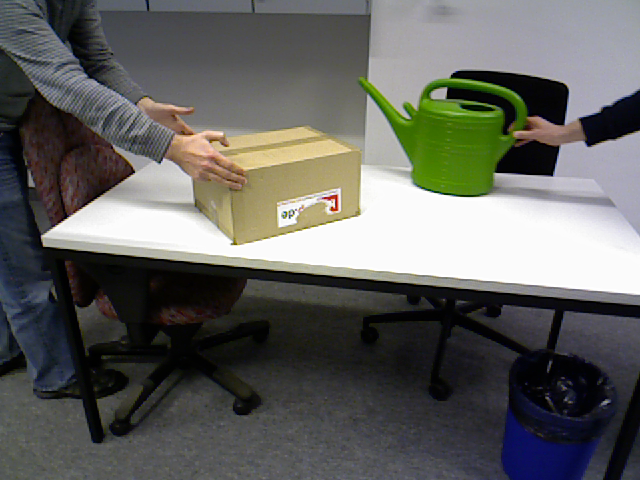
\includegraphics[width=0.22\linewidth] {evaluation/datasets/bonn_watercan/31}
}
\subfigure[Frame 58]{
   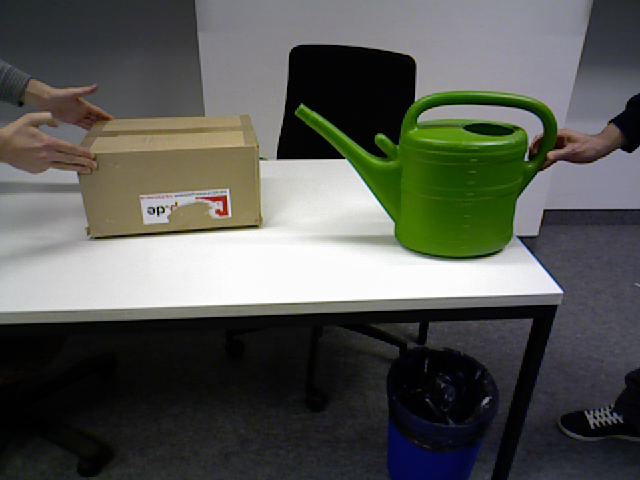
\includegraphics[width=0.22\linewidth] {evaluation/datasets/bonn_watercan/58}
}
\subfigure[GT Frame 4]{
   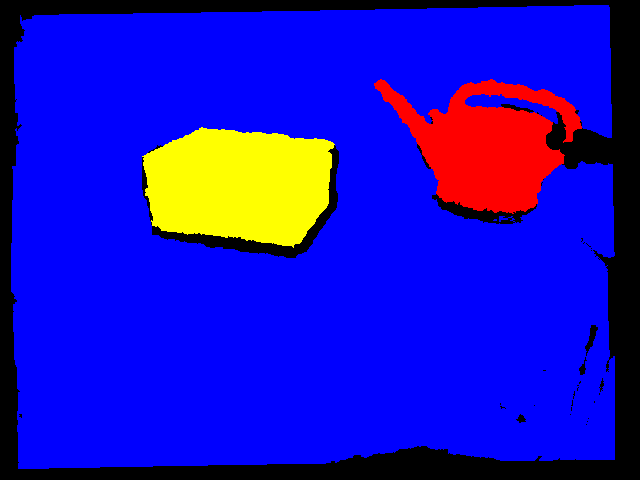
\includegraphics[width=0.22\linewidth] {evaluation/datasets/bonn_watercan/gt4}
}
\end{center}
\caption[Dataset Bonn Watercan]{An indoor scene showing two men psuhing different objects on a table. First, the man on the right side moves a water can along the table, then after a while the second man moves a packet from the left side of the table to its center. The camera is slightly shaking.}
\label{fig:eval_datasets_bonn_watercan}
\end{figure}
\item \textbf{Bonn Chairs}: \textbf{frames}: 58, \textbf{resolution}: $480 \times 640$, \textbf{depths}: Yes
\begin{figure}[H]
\begin{center}
\subfigure[Frame 15]{
   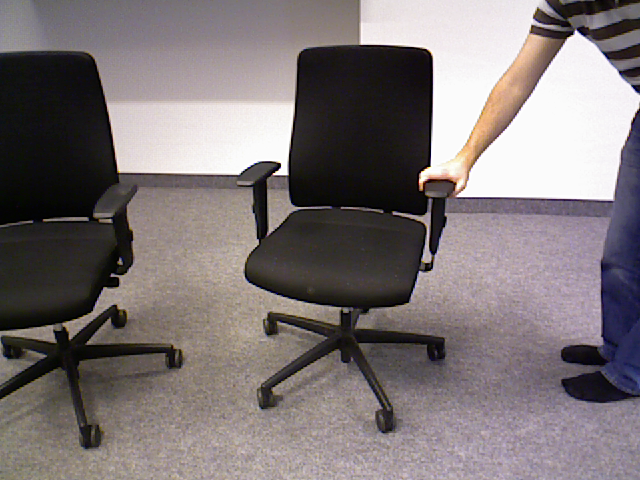
\includegraphics[width=0.22\linewidth] {evaluation/datasets/bonn_chairs/15}
}
\subfigure[Frame 30]{
   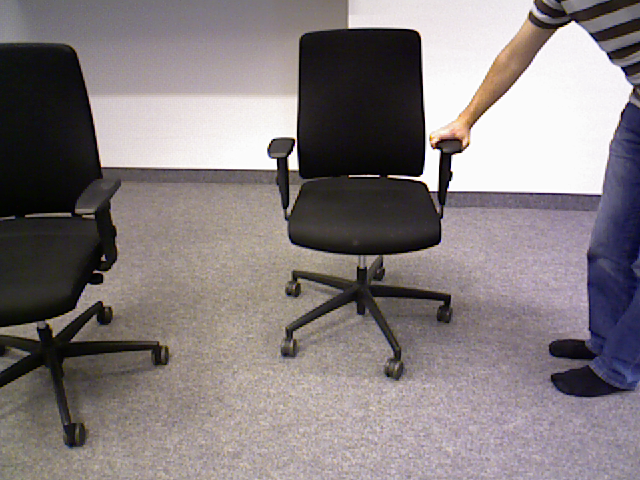
\includegraphics[width=0.22\linewidth] {evaluation/datasets/bonn_chairs/30}
}
\subfigure[Frame 45]{
   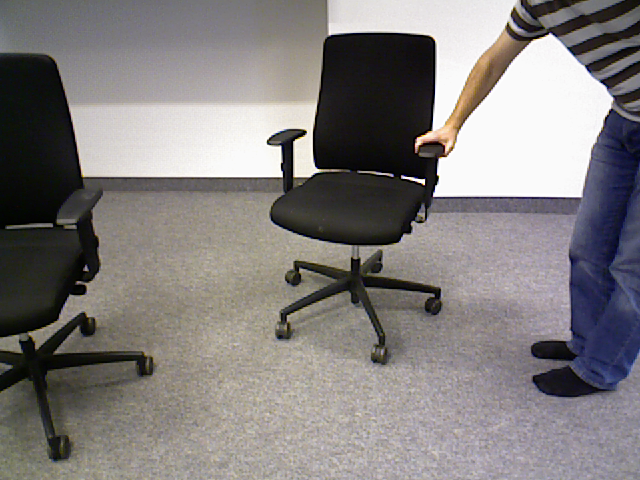
\includegraphics[width=0.22\linewidth] {evaluation/datasets/bonn_chairs/45}
}
\subfigure[GT Frame 15]{
   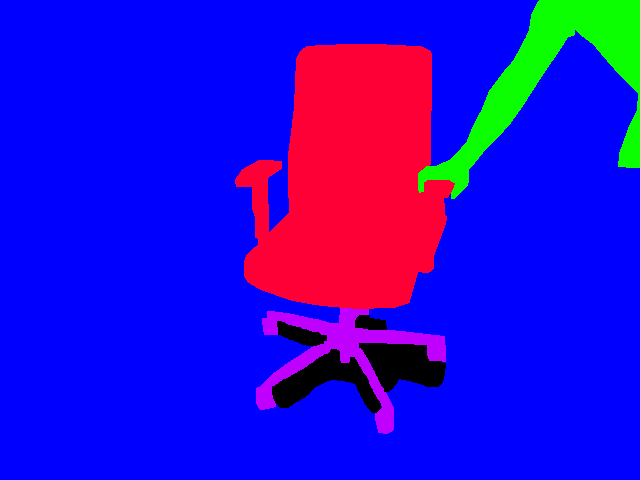
\includegraphics[width=0.22\linewidth] {evaluation/datasets/bonn_chairs/gt15}
}
\end{center}
\caption[Dataset Bonn Chairs]{An indoor scene showing a man moving a chair. First, he moved it to the left, then he rotates it slightly. The camera is slightly shaking.}
\label{fig:eval_datasets_bonn_chairs}
\end{figure}
\item \textbf{Bonn Cerealbox}: \textbf{frames}: 101, \textbf{resolution}: $480 \times 640$, \textbf{depths}: Yes
\begin{figure}[H]
\begin{center}
\subfigure[Frame 40]{
   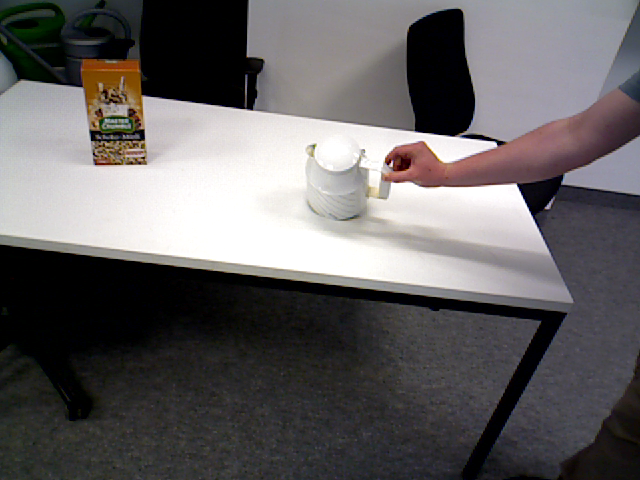
\includegraphics[width=0.22\linewidth] {evaluation/datasets/bonn_cerealbox/40}
}
\subfigure[Frame 60]{
   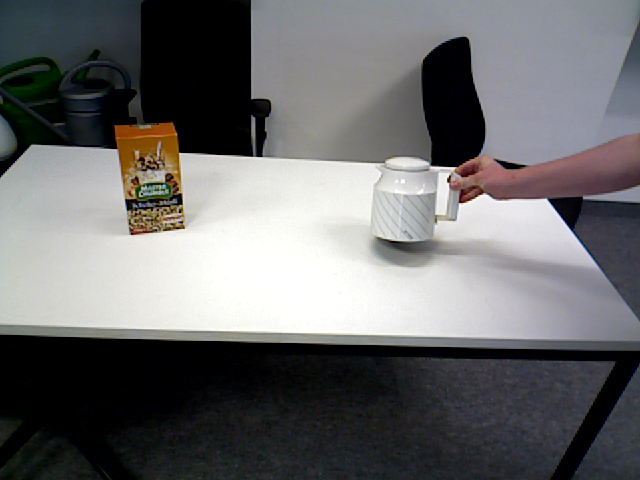
\includegraphics[width=0.22\linewidth] {evaluation/datasets/bonn_cerealbox/60}
}
\subfigure[Frame 80]{
   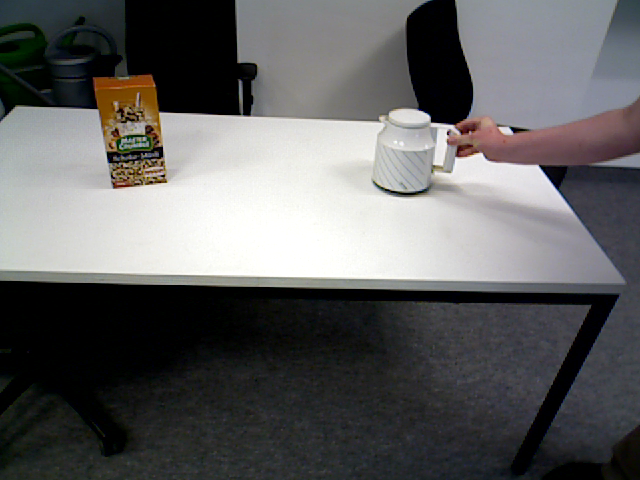
\includegraphics[width=0.22\linewidth] {evaluation/datasets/bonn_cerealbox/80}
}
\subfigure[GT Frame 40]{
   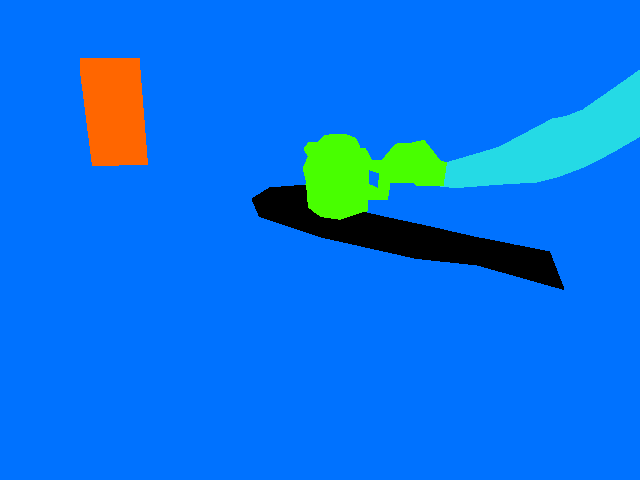
\includegraphics[width=0.22\linewidth] {evaluation/datasets/bonn_cerealbox/gt40}
}
\end{center}
\caption[Dataset Bonn Cerealbox]{An indoor scene showing a man moving a cup on table. The camera is slightly moving.}
\label{fig:eval_datasets_bonn_cerealbox}
\end{figure}
\item \textbf{Statue}: \textbf{frames}: 111, \textbf{resolution}: $480 \times 640$, \textbf{depths}: Yes
\begin{figure}[H]
\begin{center}
\subfigure[Frame 30]{
   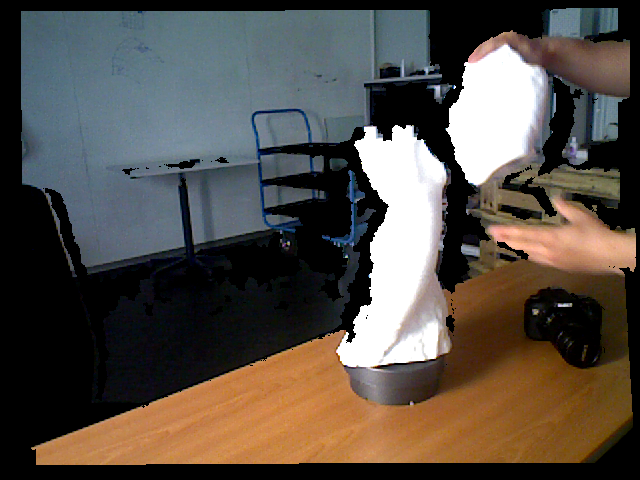
\includegraphics[width=0.22\linewidth] {evaluation/datasets/statue/30}
}
\subfigure[Frame 60]{
   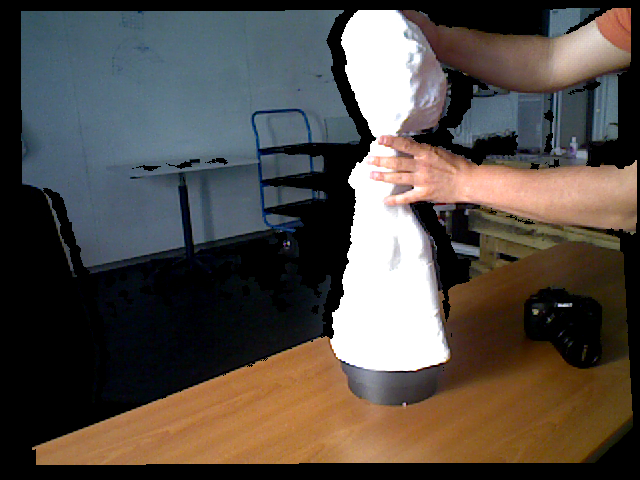
\includegraphics[width=0.22\linewidth] {evaluation/datasets/statue/60}
}
\subfigure[Frame 90]{
   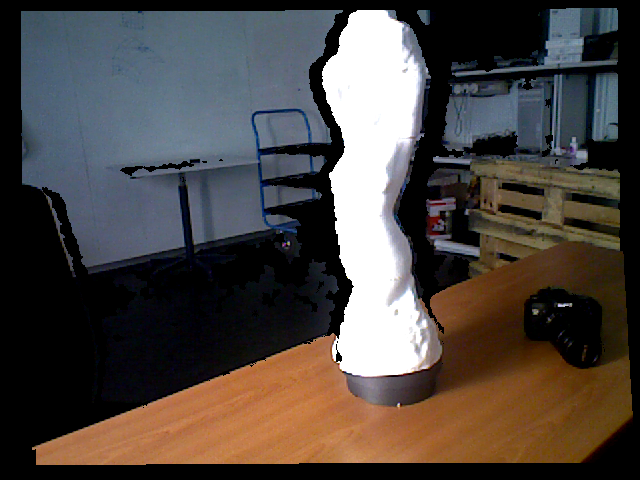
\includegraphics[width=0.22\linewidth] {evaluation/datasets/statue/90}
}
\subfigure[GT Frame 30]{
   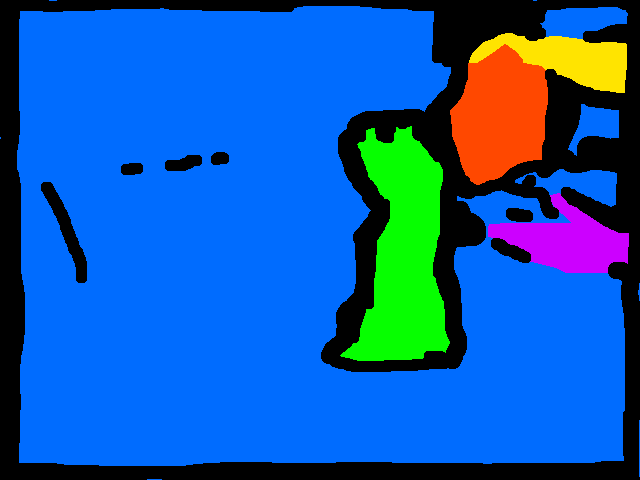
\includegraphics[width=0.22\linewidth] {evaluation/datasets/statue/gt30}
}
\end{center}
\caption[Dataset Statue]{An indoor scene a rotating statue. After a whole a man removes the upper part. We only see the man's hand. The camera is static.}
\label{fig:eval_datasets_statue}
\end{figure}
\item \textbf{Waving Arm}: \textbf{frames}: 104, \textbf{resolution}: $480 \times 640$, \textbf{depths}: Yes
\begin{figure}[H]
\begin{center}
\subfigure[Frame 20]{
   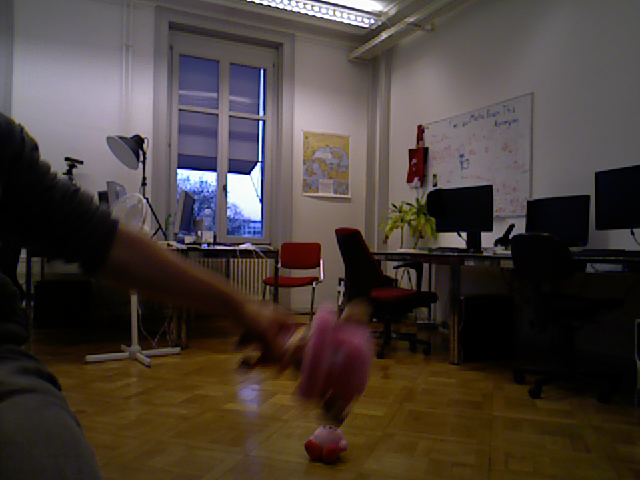
\includegraphics[width=0.22\linewidth] {evaluation/datasets/wh/20}
}
\subfigure[Frame 30]{
   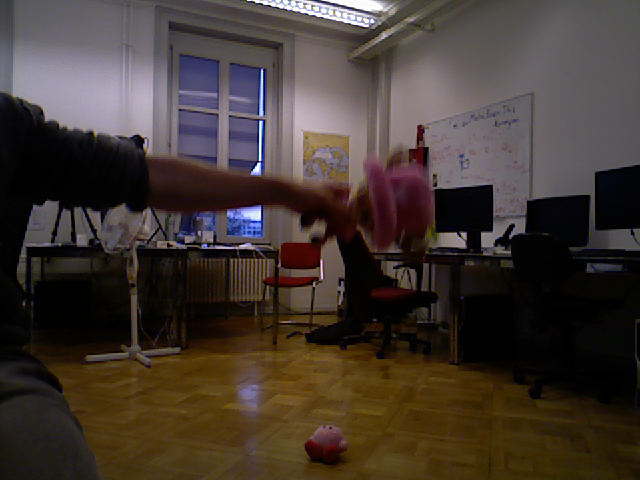
\includegraphics[width=0.22\linewidth] {evaluation/datasets/wh/30}
}
\subfigure[Frame 40]{
   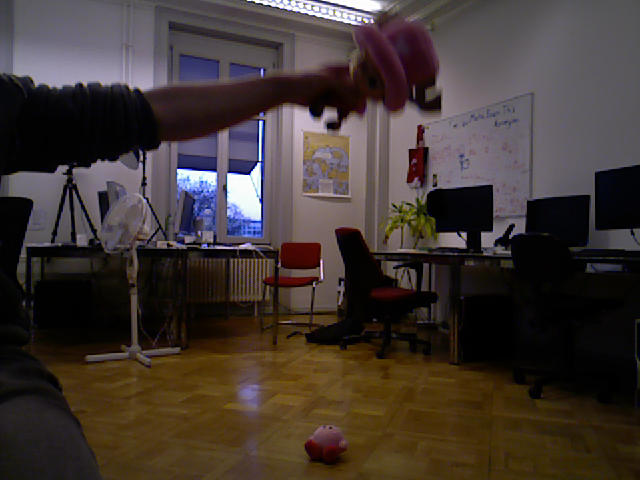
\includegraphics[width=0.22\linewidth] {evaluation/datasets/wh/40}
}
\subfigure[GT Frame 40]{
   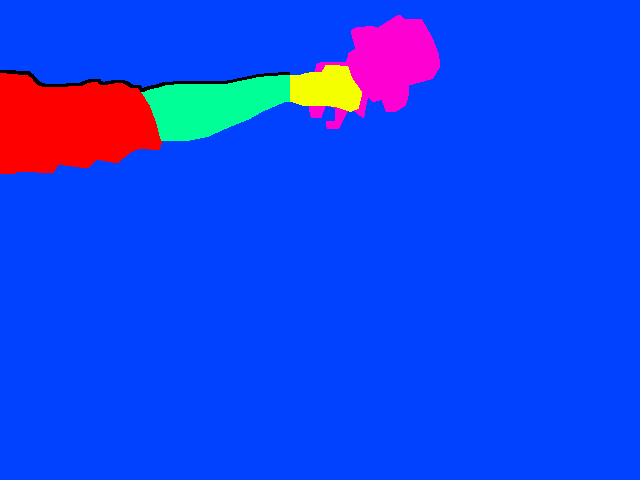
\includegraphics[width=0.22\linewidth] {evaluation/datasets/wh/gt40}
}
\end{center}
\caption[Dataset Waving Hand]{An indoor scene showing a waving arm. The camera is static.}
\label{fig:eval_datasets_waving_hand}
\end{figure}
\item \textbf{Two Chairs}: \textbf{frames}: 61, \textbf{resolution}: $512 \times 424$, \textbf{depths}: Yes
\begin{figure}[H]
\begin{center}
\subfigure[Frame 15]{
   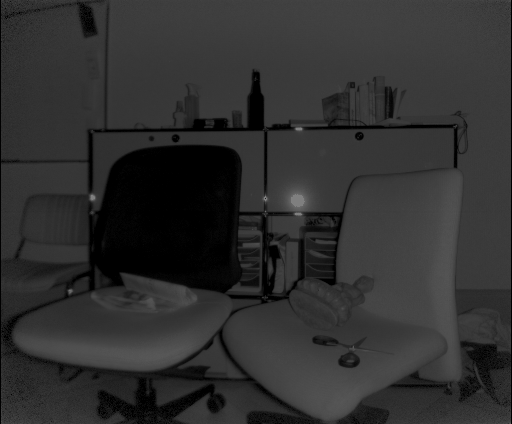
\includegraphics[width=0.22\linewidth] {evaluation/datasets/two_chairs/15}
}
\subfigure[Frame 40]{
   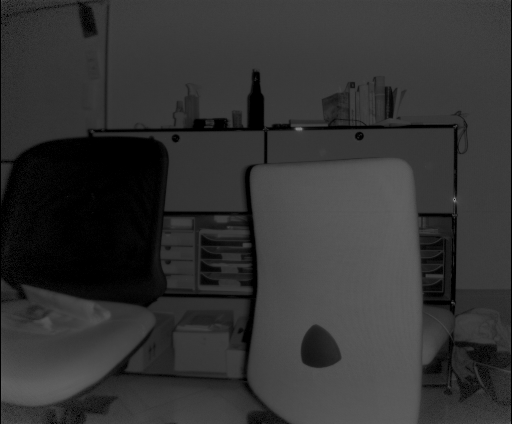
\includegraphics[width=0.22\linewidth] {evaluation/datasets/two_chairs/40}
}
\subfigure[Frame 60]{
   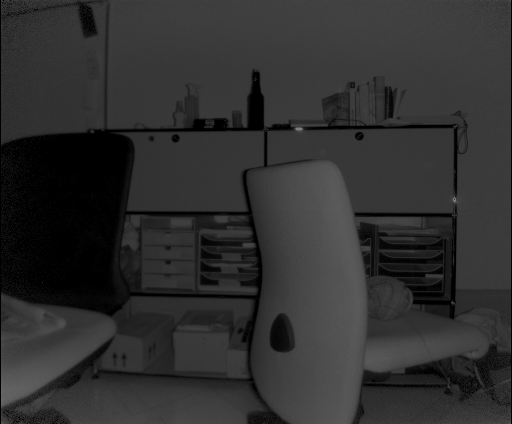
\includegraphics[width=0.22\linewidth] {evaluation/datasets/two_chairs/60}
}
\subfigure[GT Frame 15]{
   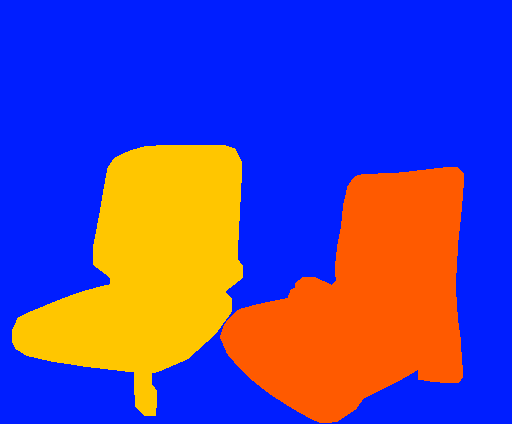
\includegraphics[width=0.22\linewidth] {evaluation/datasets/two_chairs/gt15}
}
\end{center}
\caption[Dataset Two Chairs]{An indoor scene showing two spinning chairs. The camera is static.}
\label{fig:eval_datasets_two_chairs}
\end{figure}
\item \textbf{One Chair}: \textbf{frames}: 101, \textbf{resolution}: $512 \times 424$, \textbf{depths}: Yes
\begin{figure}[H]
\begin{center}
\subfigure[Frame 45]{
   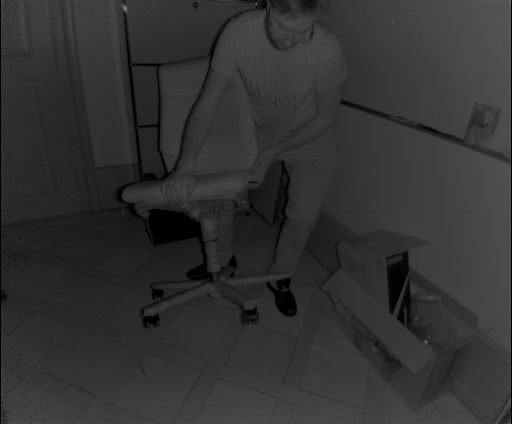
\includegraphics[width=0.22\linewidth] {evaluation/datasets/one_chair/45}
}
\subfigure[Frame 60]{
   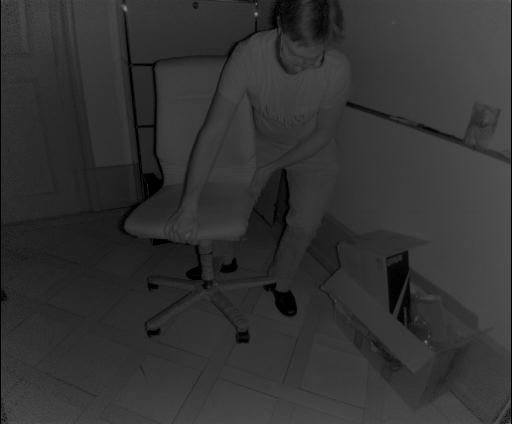
\includegraphics[width=0.22\linewidth] {evaluation/datasets/one_chair/60}
}
\subfigure[Frame 75]{
   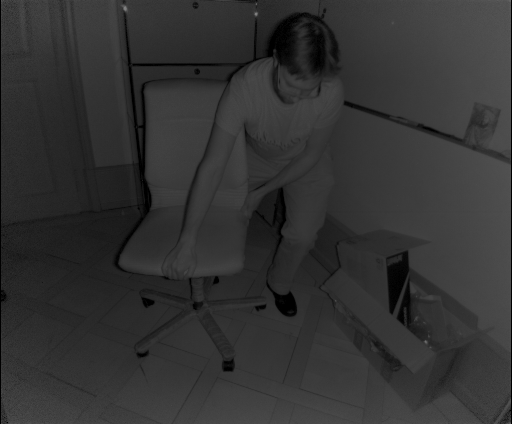
\includegraphics[width=0.22\linewidth] {evaluation/datasets/one_chair/75}
}
\subfigure[GT Frame 45]{
   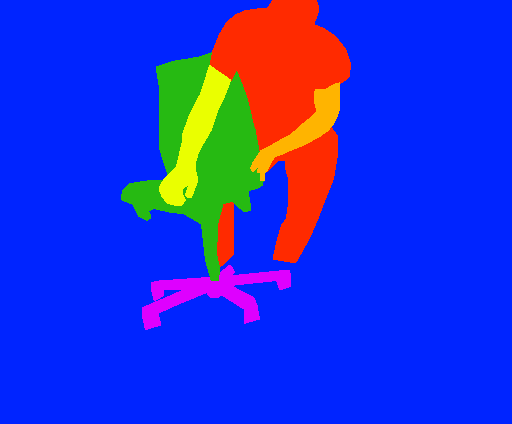
\includegraphics[width=0.22\linewidth] {evaluation/datasets/one_chair/gt45}
}
\end{center}
\caption[Dataset One Chair]{An indoor scene a man lifting a chair and spinning its lower part. The camera is static.}
\label{fig:eval_datasets_one_chair}
\end{figure}
\end{itemize}

\section{Segment Merger}
\label{sec:seg_merger}  
In this section we describe our technique to reduce oversegmentations produced by our pipeline. Our goal is to offer a mechanism that allows to evaluate the maximal potential of pipeline. However, some segmentation results are not clearly defined, such as fast movements resulting from non-rigidly moving objects. An good example of this problem case is when we attempt to segment a video showing a waving hand. That is rationale why we want to merge unclear segments. Moreover, we only allow to merger sparse segmentations, since our dense segmentation approach is basically blurring the sparse segments and thus is not yielding comparable results$\footnote{The more post-processing steps are added the more obfuscated the final segmentation quality gets.}$. This stage is invoked before running the evaluation program, implemented as a post-processing stage. \\ \\
Usually, the results generated by our pipeline exhibit an oversegmentation when comparing them against their ground truth. An example of such an oversegmentation is illustrated in figure $\ref{fig:merger_result_b}$. Ideally, before evaluating the quality, we would like to refine our over-segmented results in a way such that the total number of unnecessary or unclear segments is reduced. Therefore we want to merge  merge segments causing an oversegmentation. We achieve this by comparing the generated segments against a manually drawn ground truth image. For any generated segment we determine their best matching ground truth segment with respect to their overlapping parts. A conceptual visualization of our merging technique is visualized in figure $\ref{fig:merger_result}$. Please note that such a merging technique is just a hack. A more sophisticated method is described for merging clusters is presented in $\cite{OB14b}$.
\begin{figure}[H]
\begin{center}
\subfigure[Ground Truth Segmentation]{
   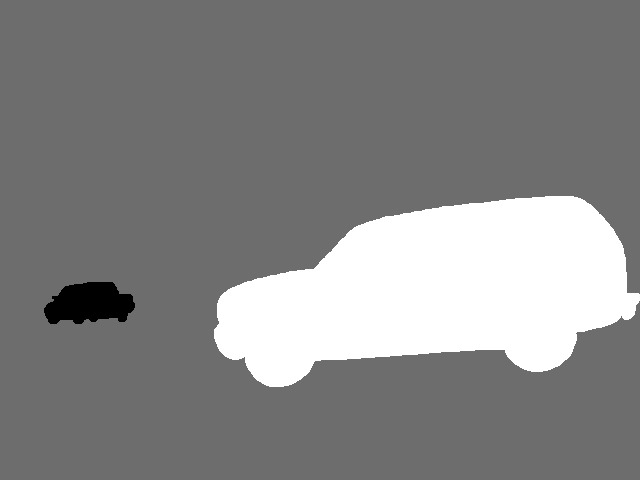
\includegraphics[width=0.47\linewidth] {implementation/merger/mask}
   \label{fig:merger_result_a}
}
\subfigure[Generated Segmentation]{
   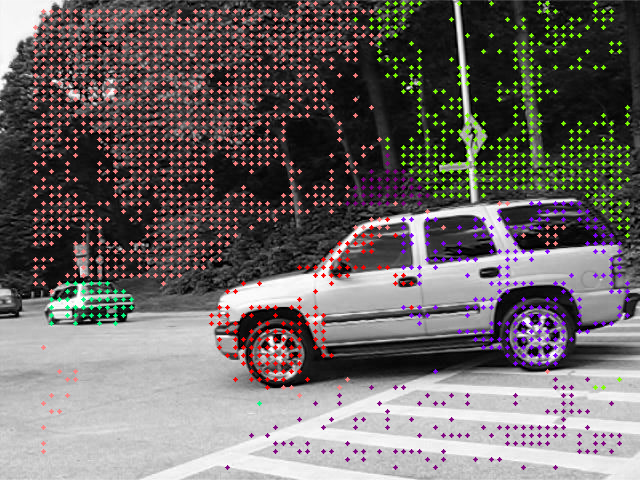
\includegraphics[width=0.47\linewidth] {implementation/merger/oversegmentation}
   \label{fig:merger_result_b}
}
~
\subfigure[Overlay Ground Truth / Segmentation]{
   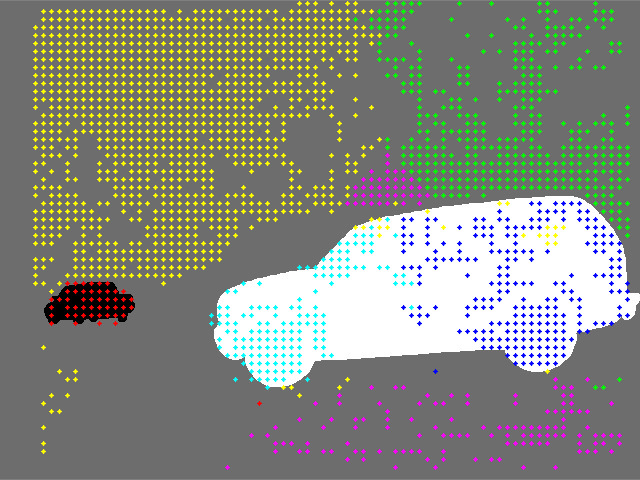
\includegraphics[width=0.47\linewidth] {implementation/merger/mask_segments_overlay}
   \label{fig:merger_result_c}
}
\subfigure[Merged Segmentation]{
   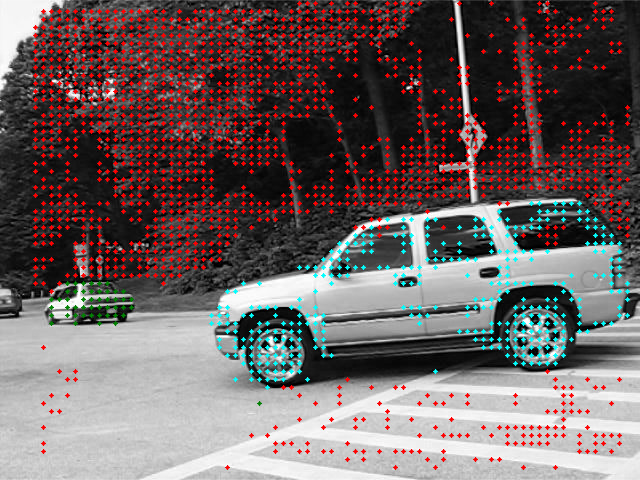
\includegraphics[width=0.47\linewidth] {implementation/merger/merged}
   \label{fig:merger_result_d}
}
\end{center}
\caption[Segmentation Merger]{Visualization of our segment merger's input and output. As an input it expects a ground truth segmentation (see figure $\ref{fig:merger_result_a}$) and a generated oversegmentation (see figure $\ref{fig:merger_result_b}$). As output it yields the merged segmentation as shown in subfigure $\ref{fig:merger_result_c}$.}
\label{fig:merger_result}
\end{figure}
A segmentation $S$ is basically a set of points in which every point is assigned to a certain segment identifier. In the following let us denote $S_j$ as the subset of points in $S$ that belong to the segmentation label $j$. Similarly, let $M$ denote the set of all ground truth points with their corresponding mask labels and $M_i$ the set of all points that belong to the ground truth mask $i$. To compute the merged segments we do the following: For every segment $S_j$ in $S$ we determine its best matching ground truth segment $M_i$ as defined in equation $\ref{eq:merging_label_formula}$. 
\begin{equation}
i = \argmaxl_{M_i \in M} \left\vert{S_j \cap M_i}\right\vert
\label{eq:merging_label_formula}
\end{equation}
The idea is to find the ground truth mask $i$ that yields the most point intersections with the currently considered segment $S_j$. Next, we update every point in $S_j$ by setting their segment label to $i$. After doing so we have computed the merged segmentation version of the initial oversegmentation. An example is shown in figure $\ref{fig:merger_result_c}$.

\section{Methodology}
\label{sec:methodology}
In this section we give a brief description about the methodology used to perform our experiments. \\ \\
We want to quantitatively evaluate the quality of segmentations produces by running different pipeline combinations. In particular we propose to evaluate the quality of how well moving objects were segmented. We use the datasets described in section $\ref{sec:datasets}$. Produced motion segmentations are compared against available ground truth images. While running the pipeline we rely on the defaults described in section $\ref{sec:spectral_clustering_parameters}$.\\ \\
Before evaluating the performance of generated segmentations, we run our segment merger, which is described in section $\ref{sec:seg_merger}$, as a post-processing step. The merged segments are quantitatively evaluated using different statistical measures. After running the merger, each GT object is assigned to at most one label. Therefore, the evaluation measures can be computed independently per object. In particular, for each segmentation result we compute their precession, recall and their f1 score by comparing them against their ground truth. The definition of these measures is listed in equation $\ref{eq:statistical_measures}$. 
\begin{equation}
\begin{aligned}
	& \text{precision} = \frac{\text{TP}}{\text{TP} + \text{FP}} \\
	& \text{recall} = \frac{\text{TP}}{\text{TP} + \text{FN}} \\
	& F_1 \text{ Score} = 2 \left( \frac{\text{precision} \times \text{recall}}{\text{precision} +\text{recall}} \right)
\end{aligned}
\label{eq:statistical_measures}
\end{equation}
The final reported outputs is the average value of these measured over all foreground objects. \\ \\
Finally some words about how we determined the quantities $TP$, $FP$ and $FN$. We only have to iterate over all points in every cluster and compare them against an available ground image. While doing so we count their true positives (\textbf{TP}), false negatives (\textbf{FP}) and their false negatives (\textbf{FN}). The exact definition of these quantities is listed in equation $\ref{eq:statistical_counts}$. For a given label $\alpha$ these measures are defined as:
\begin{equation}
\begin{aligned}
	\textbf{TP} &:= \text{Samples correctly labeled $\alpha$} \\
	\textbf{FP} &:= \text{Samples incorrectly labeled $\alpha$} \\
	\textbf{FN} &:= \text{Samples that were labeled $\alpha$ in GT but are attributed to a wrong label.}
\end{aligned}
\label{eq:statistical_counts}
\end{equation}
A detailed explanation of these measures can be found in the background section $\ref{sec:on_statistics_bg}$ on page $\pageref{sec:on_statistics_bg}$. \\ \\
One last note: During our evaluations we want to determine the quality of segmentations and the influence of design choices regardless of additional post-processing steps. Since our dense motion segmentation method basically performs a blurring on the sparse segmentation, and thus the quality is arbitrary influenced, we disallow using dense segmentations in our quantitative evaluation.

\section{Experiments}
\subsection{Parameter Experiments}
\label{sec:parameter_experiments}
In this section we describe a series of experiments that address our default parameter selection choice. In particular it acts as a justification of our choices and should demonstrate its legitimization.

Ideally, we would run every dataset on every possible pipeline combination. However, this würde den rahmen sprengen.

to justify

For illustration purp

lediglich veranschauungszweck, untermalen, warum parameter so gewählt wie erklärt

ziel: alle varianten auf allen datasets
probleme: komplexity, dh alle kreuzkombinationen, so impractical that considering ldof and srsf

hs vergleichbar mit ldof und lrgbd 

zeige ldof sed kl
plots
u dessen plots (klein für var cluster)
% convergence i, ldof ped mc

\subsubsection{Convergence MC}
In the graph of figure $\ref{fig:two_chairs_ped_mc_iterations}$ we see a plot of the convergence rate of the MC segmentation method. The more iterations we run, the higher the F1-Score gets. However, we also observe, that the F1 Score is converging already after 3 iterations. This matches with our assumption that no more than 5 to 10 iterations have to be run when using the MC segmentation method.
\begin{figure}[H]
\begin{center}
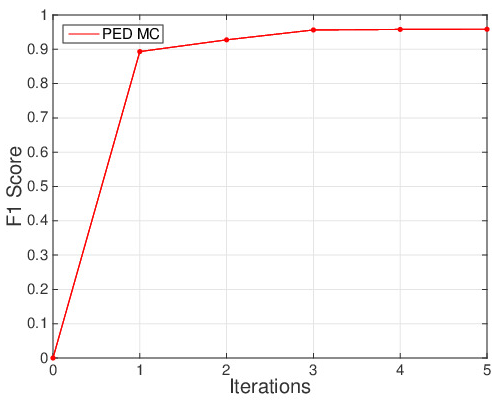
\includegraphics[width=0.47\linewidth] {evaluation/two_chairs/performance_iter/iter_f1}
\label{fig:two_chairs_ped_mc_iterations_b}
\end{center}
\caption[Convergence Rate MinCut Segmentation]{Visualizing the convergence rate of MC. We observe, that the more iterations are run, the higher the F1-Score gets. However}
\label{fig:two_chairs_ped_mc_iterations}
\end{figure}

\subsubsection{Choice for lambda}
\begin{table}[H]
\centering
\begin{tabular}{|c|c|c|c|c|}
\hline
\multicolumn{5}{|c|}{Performance Varying $\lambda$}                        \\ \hline
$\lambda$              & \textbf{Density} & \textbf{Precision} & \textbf{Recall} & \textbf{F1 Score} \\ \hline
5 & 0.59 & 99.70\%   & 57.99\%     & 73.33\%  \\ \hline
0.01 & 0.67 & 91.07\%   & 92.85\%     & 91.95\%  \\ \hline              
0.0001 & 0.67 & 47.91\%   & 49.62\%     & 48.75\%  \\ \hline
\end{tabular}
\caption[Cars Varying $\lambda$]{My caption}
\label{tab:cars_varying_lambas}
\end{table}

\subsubsection{Eigenvector Clustercount default}

\subsection{On exploring flow methods}
hs und lrgbd rausschmeisen

\subsection{Overall Performance}



\begin{table}[H]
\centering
\begin{tabular}{|c|c|c|c|}
\hline
\multicolumn{4}{|c|}{Using all datasets}                        \\ \hline
Method & \textbf{Precision} & \textbf{Recall} & \textbf{F1 Score} \\ \hline
LDOF PD SC & 63.52 \%   & 41.87\%     & 50.47\%  \\ \hline
LDOF PD MC & 58.69\%   & 57.86\%     & 58.27\%  \\ \hline
LDOF PED SC & 66.94\%   & 57.91\%     & 62.10\%  \\ \hline
LDOF PED MC & 64.11\%   & 67.27\%     & 65.65\%  \\ \hline                 
\end{tabular}
\caption[Overall Performance]{My caption}
\label{tab:overall_performance}
\end{table}


\begin{table}[H]
\centering
\begin{tabular}{|c|c|c|c|}
\hline
\multicolumn{4}{|c|}{Using compatible datasets}                        \\ \hline
Method & \textbf{Precision} & \textbf{Recall} & \textbf{F1 Score} \\ \hline
LDOF PD SC & 60.04 \%   & 35.99\%     & 45.00\%  \\ \hline
LDOF PD MC & 54.65\%   & 58.31\%     & 56.42\%  \\ \hline
LDOF PED SC & 63.85\%   & 59.68\%     & 61.69\%  \\ \hline
LDOF PED MC & 59.30\%   & 64.79\%     & 61.93\%  \\ \hline
SRSF PED MC & \textbf{76.52}\%   & \textbf{83.47}\%     & \textbf{79.84}\%  \\ \hline
SRSF PED SC & 60.23\%   & 49.62\%     & 54.41\%  \\ \hline 
SRSF PD MC & 61.85\%   & 55.06\%     & 58.25\%  \\ \hline
SRSF SED KL & 87.19\%   & 91.77\%     & 89.42\%  \\ \hline
Brox's GraphCut & 30.88\%   & 25.34\%     & 27.84\%  \\ \hline                   
\end{tabular}
\caption[Overall Performance]{My caption}
\label{tab:overall_performance}
\end{table}


\subsection{Properties}

\section{Runtime Measurements}
In this section we present actual runtime measurements resulting when running on the specified machine as defined in table $\ref{tab:used_hardware_specs}$. Please notice that by no means these measurements can be considered as statistical evident. The sole purpose of this section is to give the reader some further understanding about the pipeline and its usability in terms of \textit{how handy is this whole pipeline to use w.r.t. its runtime}. \\ \\
We start with measuring the runtimes of the utilized flow methods. For each method we run 3 dataset$\footnote{The dataset frames used to perform these measurement all exhibit a resolution 640 x 480 pixels.}$ and measured their total time to process their input. Each time measurement was divided by their total number of frames. The resulting timings were then finally averaged. Table $\ref{flow_method_runtimes}$ lists the average time in seconds that our flow methods require to process$\footnote{Here, the term process refers to generating the forward-and backward flow field of a frame.}$ one dataset frame. 
\begin{table}[H]
\centering
\begin{tabular}{|l|l|}
\hline
\textbf{Flow Method} & \textbf{Time per Frame} \\ \hline
HS & 18s \\ \hline
LDOF & 24s \\ \hline
SRSF & 72s \\ \hline
LRGBD & 674s \\ \hline
\end{tabular}
\caption[Flow Method Runtimes]{Listing of the average time of our flow methods required to process one dataset frame}
\label{flow_method_runtimes}
\end{table}
Next let us discuss the timings of the affinity matrix generation. Figure $\ref{fig:runtime_tra_track_affinity_gen}$ shows the timings in seconds of 261 measurements (blue dots) to accomplish the task of tracking a varying count of trajectories and generating their corresponding affinity matrix. Moreover, we fit a quadratic polynomial (red curve) on our measurements, since the runtime complexity of this pipeline stage is supposed to be in $\mathcal{O}(n^2)$ and $n$ denotes the trajectory count.
\begin{figure}[H]
\begin{center}
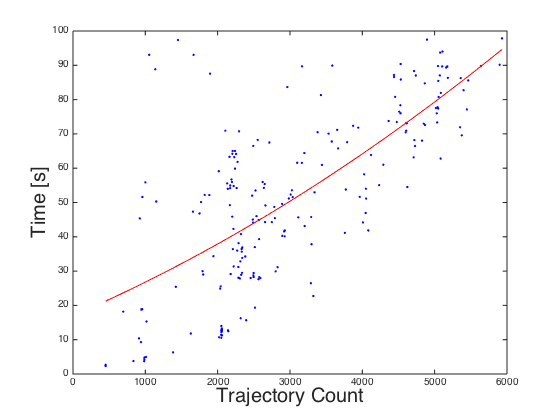
\includegraphics[width=0.8\linewidth] {evaluation/runtimes/affinity}
\end{center}
\caption[Runtime Trajectory Tracking and Generating Affinity Matrix]{Plotting the runtime (in seconds) of trajectory tracking and affinity matrix generation stage against the utilized trajectory count. The measurements are visualized as blue dots. A reconstructed quadratic curve is shown in red. The runtime of the evaluated stage is supposed to exhibit a quadratic complexity.}
\label{fig:runtime_tra_track_affinity_gen}
\end{figure}
Unfortunately, we have not performed detailed measurements for the $\textit{P-affinity}$ segmentation methods. In our pipeline we implemented the SC and MD segmentation methods in Matlab. Generally, loading an affinity matrix that represents the similarity of 1000 affinities takes 5 seconds, 3000 approximately 20 seconds and 6000 about 90 seconds. For solving the eigenvalue decomposition in our Matlab implementations, we rely on the fast numerical approximation of $\textit{eigs}$. The final k-means run in SC takes about 30 seconds when using 6000 trajectoires and performing 200 repetitions. So, the runtime of SC, using our specs takes at most two minutes. In MC the most outer loop runs a k-means step and a graph-cut step. The k-means takes about the same time as in SC. Again, when using about 6000 trajectories, then calling graph-cut in this loop takes about 3 minutes. When using the default neighborhood assignment as discussed in section $\ref{sec:spectral_clustering_parameters}$. \\ \\
In contrast, we measured the timings of several Kerninghan-Lin runs.

%TODO: list runtime performance plots of our pipeline components
%TODO: list it in a table 


\section{Discussion}
After running our pipeline the following key observations can be stated:
\begin{itemize}
  \item Our pipeline can handle complex scenes: moving cameras, rotational movement.
  \item SRSF flows achieve the best segmentation results
  \item however, LDOF flows are still a solid choice and yield competitive results.
  \item when using P-affinities, then use Min-cut segmentation
  \item SED KL achieves the best results
  \item the best pipeline combination is SRSF SED KL 
  \item LRGBD flows are a very bad choice and yield poor motion segmentations
  \item using depth fields improves the quality of the segmentation results drastically
  \item when comparing our default pipeline setup against Brox' Min-Cut method, we obtain way better results.
  \item choosing the correct number of clusters and segments is a non-trivial task.
\end{itemize}












\newpage{\pagestyle{empty} \cleardoublepage}

\chapter{Conclusion}
\section{Summary}
In this thesis we implemented a pipeline that can successfully perform the task of motion segmentation on RGB-D sequences using optical flows. For this purpose many, commonly known from literature, different techniques for generating the flows, computing affinities between trajectories and for performing the actual segmentation task were implemented and examined. \\ \\
We statistically evaluated the quality of all possible pipeline combinations on various dataset by comparing the resulting segmentations against manually generated ground truth images. This way we were able to determine the strengths and weaknesses of different techniques and find an optimal setting. \\ \\
Especially, we were able to show quantitatively, that incorporating depth cues into the individual pipeline components drastically improves the quality of the resulting motion segmentations. Moreover, we observed that the quality of the utilized flows significantly affects the segmentation quality. Hence, we concluded, that when using P-affinities, our best pipeline setup is $\text{SRSF PED MC}$ and when using S-affinities $\textit{SRSF SED KL}$. Both variants achieve best results compared against the other available setups. However, SRSF SED KL achieves better f1 scores but SRSF PED MC runs much faster. Therefore, we denote both methods as winners.  \\ \\
Moreover, when using our best pipeline setups, we could deal with complex scenes, which exhibit camera shaking, rotational movements and even slight non-rigid movements. Additionally, our pipeline is also capable of dealing with noise in the flow fields by using various filters. Therefore, we conclude that we were able to fulfill our initially stated goals. \\ \\
Regarding the limitations of this work we can state the following main issues: Our implementation is a over-paramterized pipeline. Many parameter values are chosen according to simple heuristics. For example the number of moving objects we want to solve for in our segmentation methods is assigned manually for each dataset. The same holds true for the number of neighbors that should be used for various stages, the number of eigenvectors and the values of $\lambda$ used to compute P-affinities, as well as the prior cut probability used to compute S-affinities. Another issue is the runtime of several pipeline components. For example the Kernighan Lin implementation has a poor runtime which could drastically be improved State paper REF. Next, our segment merger method requires ground truth images of particular frames to work correctly. However, relying on a sophisticated method as described in $\cite{OB14b}$ would be more reliable. Lastly, we could adapt the pairwise affinity computation model by replacing it by a higher order model, similar as described in $\cite{OB12}$. \\ \\
Regarding future work we could think of many useful extensions and enhancements that directly address the stated limitations. The most beneficial extension, however, would be to automatically determine the optimal parameter setup using a learning based approach. Moreover, the pipeline could be adapted in a way to let it run at interactive rates by porting the code to a GPU implementation. Since the quality of the optical flows strongly influences the resulting segmentations, we also could think of refine the flow estimation by a method that combines LDOF and SRSF. This would yield a method that is capable of dealing with large motion as well as utilizing depth cues to deal with rotational movements and deformation. Lastly, we could think of developing a special neuronal network, which is capable of estimating depth maps by using a single color image. This idea is based on the work from paper $\cite{DBLP:journals/corr/EigenPF14}$.  

\section{Personal Experience}
After having successfully written my bachelor thesis at the Computer Graphics Group at the University of Bern, I was certain that, eventually, I would like to write my master thesis in a related field of Computer Graphics and Vision. Since I am generally very interested in topics like numerics and optimization problems, I asked for a thesis subject that combines Mathematics with practical problem. I have to admit that, after having read papers about segmentation techniques and variational methods at the very beginning of my thesis, I thought this topic would exceed my knowledge. And it actually did, but I decided not to give up. \\ \\
During working on my thesis I learnt many new concepts in Mathematics relating to optical flow, motion segmentation, clustering and graph partitioning methods, solving optimization problems and deepened my knowledge of numerics. I felt it as a satisfactory experience to use and apply all the knowledge which I have acquired during the time as a bachelor and master student. Furthermore, this thesis gave me the opportunity to program quite a lot. Hence I could strengthen my programming skills in Java and C++, Matlab and Ruby. Altogether it was a rewarding experience for me to write a Master thesis at the Computer Graphics Group.
\section{Acknowledgment}
First, I would like to thank Mr. Zwicker for giving me the opportunity to write a Master thesis at the Computer Graphics Group at the University of Bern. \\ \\
Foremost, I would like to express my sincere gratitude to my advisor Mr. Peter Bertholet for his continuous support of my study, his patience, motivation, enthusiasm, and knowledge. His guidance and active support helped me quite a lot while deriving the necessary formulations used by our pipeline, implementing them and evaluating the motion segmentations. \\ \\
Last but not least, I would like to thank my mother, Manuela Single and my brother Patrik Single and also to my close friend, Radischa Iyadurai for supporting me morally throughout during this thesis.
\newpage{\pagestyle{empty} \cleardoublepage}

\begin{appendix}
\chapter{Additional Pipeline Information}
\section{Corner thresholding}
\label{sec:corner_thresholding}
describe the corner thresholding approach here.

\section{Depth Field Variances}
\label{sec:depth_field_variances}
describe how depth field variances can be computed and how they can be used. Additionally, describe the run-mode in the pipeline and maybe also offer some results and limitations.

\chapter{Additional Theoretical Background}
\section{On Filtering Images}
\subsection{Gaussian Filter}
A Gaussian filter (\textbf{GF}) is a linear operator that reduces noise by smoothing the image. Applying GF corresponds to a low-pass filtering.
At each position it estimates a local average of the intensities as defined in equation $\ref{eq:gaussian_filtering_def}$.
\begin{equation}
	\mathcal{F}^{\text{gf}} \{I \} (p) = \sum_{q \in \Omega_p} G_{\sigma} (\norm{p - q}) I_q
\label{eq:gaussian_filtering_def}
\end{equation}
where $I$ defines the input image and $\Omega_p$ contains all neighboring points within the window that are centered at the image point $p$. Moreover, $G_{\sigma}$ denotes the two dimensional Gaussian kernel, which is defined in equation $\ref{eq:def_g_weight}$.
\begin{equation}
	G_{\sigma} (x) = \frac{1}{2 \pi \sigma^2} e^{-\frac{x^2}{2 \sigma^2}}
\label{eq:def_g_weight}
\end{equation}
The Gaussian filtering is the weighted average of the intensity of the adjacent positions with a weight decreasing with the spatial distance to the center position. This distance is defined by $G_{\sigma} (\norm{p - q})$ where $\sigma$ is a parameter that defines the size of the neighborhood. The resulting image is a blurred version of the input image.

\subsection{Bilateral Filter}
A Bilateral filter (\textbf{BF}) is a non-linear operator that reduces noise by smoothing the image but at the same time preserves its edges. \\ \\
The rational of this filter is that two pixels are close to each other if not only if their spacial distance is small but also if they are similar regarding their intensity range.
\begin{figure}[H]
\begin{center}
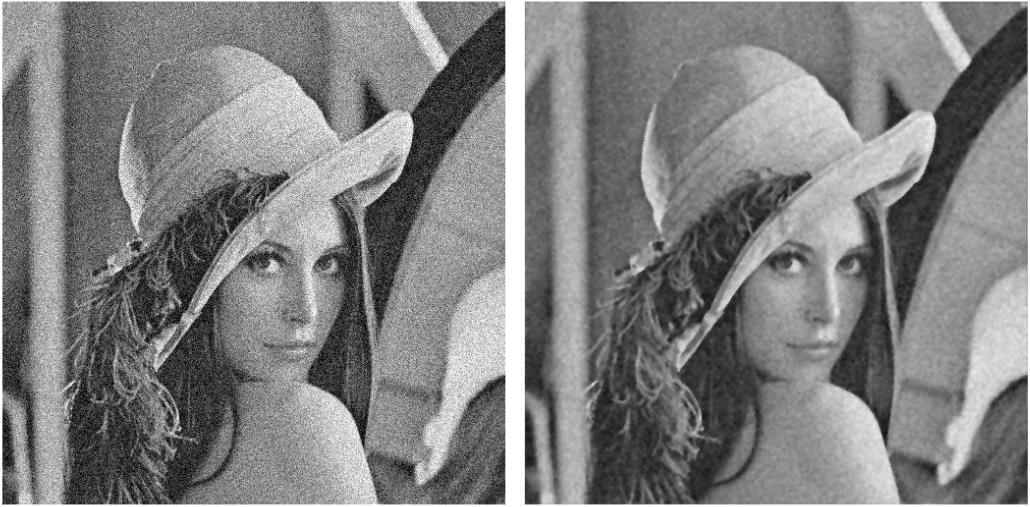
\includegraphics[width=0.6\linewidth] {background/filtering/bilat_filter_eg}
\end{center}
\caption[Example Bilateral Filter]{A bilateral filtering example$\footnotemark$: On the left side a noisy input image on the right its bilateral filtered version.}
\label{fig:bilat_filtering_eg}
\end{figure}
\footnotetext{The shown images have been extracted from: \\ \url{https://www.uni-due.de/mathematik/krommweh/talk_Gemen_Krommweh.pdf}}
The filter replaces the intensity values at each pixel in an image by a weighted average of intensity values from nearby pixels. In our formulation we rely on the Gaussian distributions $G$ for defining the weights. Crucially, the weights depend not only on distances between pixels, but also on the intensity difference. That is why, when iterating through each pixel and adjusting weights to the adjacent pixels accordingly, Sharp edges are preserved. A bilateral filtering example is shown in figure $\ref{fig:bilat_filtering_eg}$.\\ \\
The mathematical definition of this filter is given in equation $\ref{eq:def_bilateral_filter}$. For a given Image $I$ we want to compute its bilateral filtered version by applying the following definition:
\begin{equation}
\begin{aligned}
&\mathcal{F}^{\text{bf}} \{I \} (p) = \frac{1}{W_p} \sum_{q \in \Omega_p} G_{\sigma_s} (\norm{p-q})G_{\sigma_r} (I_p - I_q) I_q \\	
& \text{where } W_p = \sum_{q \in \Omega_p} G_{\sigma_s} (\norm{p-q})G_{\sigma_r} (I_p - I_q)
\end{aligned}
\label{eq:def_bilateral_filter}
\end{equation}
The set $\Omega_p$ contains all neighboring points within the window that are centered at the image point $p$. The scalar $W_p$ denotes the normalization factor of the filter and $I_p$ represents the image intensity at the pixel position $p$. Please notice that the definition of the bilateral filter is given per pixel, i.e. gives an representation of the filtered pixel intensity. \\ \\
The bilateral filter is controlled by the two parameters $\sigma_s$ and $\sigma_r$. The range variance increases $\sigma_r$, the BF becomes closer to the Gaussian blur filter. In other words, the larger $\sigma_r$ the more weight a pixel with a large intensity deviation gets. However, when increasing the spatial variance $\sigma_s$ results in smoothing larger features, i.e more distant pixels get a larger weight and thus influence the result more. Figure $\ref{fig:bfilter_influence_sigmas}$ demonstrates the influence of these parameters.
\begin{figure}[H]
\begin{center}
\includegraphics[width=0.6\linewidth] {background/filtering/bilat_filter_sigmas}
\end{center}
\caption[Influence of $\sigma_s$ and $\sigma_r$]{Different filtering results produced by our bilateral filter implementation for varying $\sigma_s$ and $\sigma_r$ values.}
\label{fig:bfilter_influence_sigmas}
\end{figure}

\subsection{Harris Corner Detector}
\label{sec:harris_corner_detector}
Let us consider a grayscale image $I$. We are going to sweep a window $w(x,y)$ (with displacements u in the x direction and v in the right direction) I and will calculate the variation of intensity. Since we are looking for windows with corners, we are looking for windows with a large variation in intensity. Hence, we have to maximize the equation above, specifically the term:
\begin{equation}
	E \left( u, v \right) = \sum_{x,y} w \left( x,y \right) \left[ I(x + u, y + v) - I(x, y) \right]^2
\label{eq:var_intensitiy_def}
\end{equation}
Next, the term $I(x + u, y + v)$ is expressed by the first order taylor series expansion as the follows:
\begin{equation}
	I(x + u, y + v) = I(x,y) + u I_x (x, y) + v I_y (x,y) + \text{h.o.t}
\label{eq:taylor_exp_intensity}
\end{equation}
Next, we put the first order approximation of equation $\ref{eq:taylor_exp_intensity}$ into equation $\ref{eq:var_intensitiy_def}$ to simplify the definition of $E$.
\begin{equation}
\begin{aligned}
E \left( u, v \right) 
&= \sum_{x,y} w \left( x,y \right) \left[ I(x + u, y + v) - I(x, y) \right]^2 \\
&\approx \sum_{x,y} w \left( x,y \right) \left[ I(x,y) + u I_x (x, y) + v I_y (x,y) - I(x, y) \right]^2 \\
&= \sum_{x,y} w \left( x,y \right) \left[ u I_x (x, y) + v I_y (x,y) \right]^2 \\
&= \sum_{x,y} w \left( x,y \right) u^2 I_x^2 + 2 u v I_x I_y v^2 I_y^2 \\
&= \left( u,v \right) \left( \sum_{x,y} w (x,y)
\begin{pmatrix}
I_x^2 & I_x I_y \\
I_x I_y & I_y^2 \\
\end{pmatrix}
\right) \colvec{u}{v}
\end{aligned}
\label{eq:var_intensitiy_developed}
\end{equation}
Let us define the following substitution
\begin{equation}
M = \sum_{x,y} w  (x,y)
\begin{pmatrix}
I_x^2 & I_x I_y \\
I_y^2 & I_x I_y \\
\end{pmatrix}
\label{eq:var_intensity_sub}
\end{equation}
Putting the substitution from equation $\ref{eq:var_intensity_sub}$ into the final form of equation $\ref{eq:var_intensitiy_developed}$ we obtain the final form
\begin{equation}
	E \left( u, v \right) \approx \left( u,v \right) M \colvec{u}{v}
\end{equation}.
A score is calculated for each window, to determine if it can possibly contain a corner:
\begin{equation}
\begin{aligned}
& R = \det(M) - \kappa \left(\text{trace}(M)\right)^2 \\
&\text{where } \det(M) = \lambda_1 \lambda_2 \text{ and } \text{trace}(M) = \lambda_1 + \lambda_2
\end{aligned}
\label{eq:harris_response}
\end{equation}

\section{On Statistics}
\label{sec:on_statistics_bg}

\subsection{Conditional Probability}
Given two events $A$ and $B$ with the probability $P(B) > 0$. The conidtional probability of $A$ given $B$ is defined as
\begin{equation}
	P(A|B) = \frac{P(A \cap B)}{P(B)}
\label{eq:conditional_prob}
\end{equation}
Furthermore, equation $\ref{eq:conditional_prob}$ gives us an alternative interpretation of the probability of an intersection
\begin{equation}
P(A \cap B) = P(A|B)P(B) 	
\end{equation}
The probability that two events happen the same time is the same as the Probability of the event A given B times the probability of event B. Sticking to this definition, we can visualize all possible outcomes of two events happening the same time as shown in figure $\ref{fig:prob_tree_diagram}$.
\begin{figure}[H]
\begin{center}
\includegraphics[width=0.45\linewidth] {background/statistics/probability_tree_diagram}
\end{center}
\caption[Probability Tree Diagram]{Tree liked representation$\footnotemark$ of the four possible outcomes for a conditional probability.}
\label{fig:prob_tree_diagram}
\end{figure}
\footnotetext{The visualized graphic has been taken from: \url{https://en.wikipedia.org/wiki/File:Probability_tree_diagram.svg}}



\subsection{Evaluating Binary Classifiers}
In this section we explain the mathematical framework we use in our evaluation.


The purpose of a binary classifier is to classify given elements into two groups according to a specified classification rule. Think about a binary random variable modelling a certain event. The actual observations of the random variable are then either equals true or false. A classification$\footnote{I.e. the produced output after applying the classifier on the given data.}$ of a given dataset yields two numbers: the number of the positives and negatives, which add up to the size of the set. \\ \\
In order to evaluate the quality of binary classifier its prediction is compared against a standard reference method or, if existing, against a ground truth assignment and then cross tabulates the data into a $2 \times 2$ contingency table as shown in figure $\ref{tab:prediction_sensitivity}$. 
\begin{table}[H]
\centering
\begin{tabular}{c|c|c|}
\cline{2-3}
 & \begin{tabular}[c]{@{}l@{}}Prediction\\ Positive\end{tabular} & \begin{tabular}[c]{@{}l@{}}Prediction\\ Negative\end{tabular} \\ \hline
\multicolumn{1}{|l|}{\begin{tabular}[c]{@{}l@{}}Condition\\ Positive\end{tabular}} & \cellcolor[HTML]{34FF34}{\color[HTML]{000000} $\bf{TP}$ } & \cellcolor[HTML]{CB0000} $\bf{FN}$ \\ \hline
\multicolumn{1}{|l|}{\begin{tabular}[c]{@{}l@{}}Condiation\\ Negative\end{tabular}} & \cellcolor[HTML]{CB0000}{\color[HTML]{000000} $\bf{FP}$ } & \cellcolor[HTML]{34FF34} $\bf{TN}$ \\ \hline
\end{tabular}
\caption[Conditional Probability]{The four possible outcomes of a conditional probability}
\label{tab:prediction_sensitivity}
\end{table}
There are four possible outcomes: the classifier prediction, which has either are positive or negative condition, was actually correct or incorrect. \\ \\
Let us consider the following example where we test some people for the presence of a disease. Some of these people have the disease, and the test correctly detects them. These findings are called true positives (\textbf{TP}). Some have the disease, but the test incorrectly claims that they do not have it. These results are called false negatives (\textbf{FN}). Some people do not suffer from the disease and the test classifies correctly as health. These results are called true negatives (\textbf{TN}). And Lastly, some healthy people who are incorrectly classified as infected. These are the so called false positives (\textbf{FP}) results. \\ \\
There are many metrics that can be used to measure the performance of a classifier. In the following a listing of some prominent metrics
%
\begin{itemize}
\item \textbf{Precision}: Tells us what proportion of patients we diagnosed as having the disease actually had that disease. In other words, proportion of TP in the set of positive disease diagnoses. This is given by the rightmost column in the confusion matrix.
\begin{equation}
	\text{precision} = \frac{\text{TP}}{\text{TP} + \text{FP}}
\label{eq:def_precision}
\end{equation}
\item \textbf{Recall}: Tells us what proportion of people that actually had the disease were diagnosed by the test as having the disease. In other words, proportion of TP in the set of true disease states. This is given by the bottom row in the confusion matrix.
\begin{equation}
	\text{recall} = \frac{\text{TP}}{\text{TP} + \text{FN}}
\label{eq:def_recall}
\end{equation}
\end{itemize}
A visualization of these measures is given in figure $\ref{fig:eval_concept_recall_precc}$.
\begin{figure}[H]
\begin{center}
\includegraphics[width=0.6\linewidth] {evaluation/prec_recall}
\end{center}
\caption[Concept Recall and Precision]{This figure illustrates graphically the concept of Recall (\textbf{R}) and Precision (\textbf{P}). When estimating the sampling of a binary random variable, there are basically four possible outcomes: The we predicted it being true and it is true (\textbf{TP}), we predicted it true but it is false (\textbf{FP}), we predicted it false and it was actually negative (\textbf{FN}) or we predicted it to be true but it was actually false (\textbf{TN}). }
\label{fig:eval_concept_recall_precc}
\end{figure}
An alternative measure is the $F_1$ score. This measure is often used in determining the performance of classification tasks in machine learning. To compute its score, this measure takes into account both, the precision and the recall of the test. The exact definition of the F1 measure is given in equation $\ref{eq:f1_score}$.
\begin{equation}
F_1 = 2 \left( \frac{\text{precision} \times \text{recall}}{\text{precision} +\text{recall}} \right)
\label{eq:f1_score}
\end{equation}  
The F1 score can be interpreted as a normalized weighted average of the precision and recall measures. The best possible F1 score is equals 1 and its worst value is 0.

\section{Camera Model}
\subsection{Pinhole Camera}
A camera projects a 3d scene in a 2d image. A simple mathematical model to describe such a mapping from the 3d scene space to the 2d image space is the pinhole camera model. This model is conceptually illustrated in figure $\ref{fig:pinhole_camera_model}$.
\begin{figure}[H]
\begin{center}
\includegraphics[width=0.8\linewidth] {background/camera_model/pinhole_camera}
\end{center}
\caption[Pinhole Camera Model]{Visualizing the pinhole camera model. The camera center $C$ represents an infinitely small aperture hole and assumed to be located at $(0,0,0)$, $f$ is the focal length in pixel units, $p$ is the principal point in images coordinates, $\textbf{A} = (X, Y, Z)$ a 3d point in the scene and $\textbf{a} = (f \frac{X}{Z}, f \frac{Y}{Z})$ its projected pixel version mapped onto the image plane.}
\label{fig:pinhole_camera_model}
\end{figure}
The aperture is an infinitely small hole and there is no lens used to focus light. Therefore, lens distorting or depth of field effects are ignored. The intersection point where all rays meet is the center of the perspective projection and usually referred by \textit{camera center}. The principal axis is formed by the line perpendicular to the image plane, which passes though the camera center. Its intersection point with the image plane is called principal point. The distance between the camera center and the principal point is the so called focal length.

\subsection{Camera Parameters}
\paragraph{Intrinsic Parameters} Let $\textbf{X} = (X,Y,Z,1)^T$ denote a point in a 3D scene and $\textbf{x} = (x,y,1)^T$ its projected version in the image plane. Both points are written in their homogeneous form. The mapping from a scene point to the image plane is defined as
\begin{equation}
\textbf{x} = 
\begin{pmatrix}
f & s & p_x & 0 \\
0 & f & p_y & 0 \\
0 & 0 & 1 & 0
\end{pmatrix}
\textbf{X}
\end{equation}
where $f$ denotes the focal length and $p = (p_x, p_y)^T$ the offset to the origin in image coordinates with respect to the principal point. In modern cameras, the skew $s$ is usually equals zero. The parameters $f$, $p_x$, $p_y$ and $s$ are called \textit{intrinsic camera parameters}. Notice, that $\textbf{X}$ is expressed in terms of camera coordinates and similarly, $\textbf{x}$ in pixel coordinates.

\paragraph{Extrinsic Parameters} In general, a camera is not located at the origin of the world coordinate system and can have an arbitrary orientation. Let $\textbf{X}_w$ denote a point, living in an arbitrary camera coordinate system. To express this point in the regular camera coordinate system, we have to apply a certain transformation. In a rigid object model, the points $\textbf{X}$ and $\textbf{X}_w$ can be transformed to one another by applying a linear transformation that consists of a rotational matrix $R$ and a translation $t$. The actual mapping is defined as
\begin{equation}
	X = \left[ R | t \right] X_w
\end{equation}
The parameters $t$ and $R$ are called \textit{extrinsic camera parameters}.


%%% CLEAN UP
\chapter{Experiments}
In this section we list the results of a series of experiments we performed running our pipeline on the presented dataset from section $\ref{sec:datasets}$ on page $\pageref{sec:datasets}$. The results are evaluated according the previously explained measures from section $\ref{sec:methodology}$ on page $\pageref{sec:methodology}$. \\ \\
For performing our experiments we used MacBook Pro. The hardware specifications of this machine are listed in table $\ref{tab:used_hardware_specs}$. 
\begin{table}[H]
\centering
\begin{tabular}{|l|c|}
\hline
\multicolumn{2}{|c|}{\textbf{Hardware Specifications}} \\ \hline
\textbf{CPU} & 2.5 GHz Intel Core i7 \\ \hline
\textbf{Threads} & 8 \\ \hline
\textbf{MEMORY} & 16 GB 1600 MHz DDR3 \\ \hline
\textbf{GPU} & Intel Iris Pro 1536 MB \\ \hline
\end{tabular}
\caption{A listing of the hardware specifications of the used machine to produce the results.}
\label{tab:used_hardware_specs}
\end{table}

\subsection{Varying Pipeline Combinations for LDOF flows}
%START EXPERIMENT SETUP
chairs dataset
use only LDOF flows
affinity generation / segmentation techniques combinations
pipeline modes: PD SC, PD MC, PED SC, PED MC, SD KL, SED KL.
solve for 10 fixed clusters and evaluate the resulting segments on two different kinds of masks: real and simple case.
Which setting is the best?

moreover, evaluate the quality of LDOF SED KL segmentation by altering the number of clusters we want to solve for.
% END EXPERIMENT SETUP


The \textit{Bonn Chairs} dataset is a video sequence consisting of 58 frames. It shows a room containing two chairs and a man. The man is moving the and rotating the right chair. Also, the camera is moving. See figure $\ref{fig:eval_bonn_chairs_frames}$ to get a better understanding of the whole scene.
\begin{figure}[H]
\begin{center}
\subfigure[Frame 1]{
   \includegraphics[width=0.31\linewidth] {evaluation/bonn_chairs_frames/1}
   \label{fig:eval_bonn_chairs_frames_a}
}
\subfigure[Frame 12]{
   \includegraphics[width=0.31\linewidth] {evaluation/bonn_chairs_frames/12}
   \label{fig:eval_bonn_chairs_frames_b}
}
\subfigure[Frame 24]{
   \includegraphics[width=0.31\linewidth] {evaluation/bonn_chairs_frames/24}
   \label{fig:eval_bonn_chairs_frames_c}
}
~
\subfigure[Frame 35]{
   \includegraphics[width=0.31\linewidth] {evaluation/bonn_chairs_frames/35}
   \label{fig:eval_bonn_chairs_frames_a}
}
\subfigure[Frame 47]{
   \includegraphics[width=0.31\linewidth] {evaluation/bonn_chairs_frames/47}
   \label{fig:eval_bonn_chairs_frames_b}
}
\subfigure[Frame 58]{
   \includegraphics[width=0.31\linewidth] {evaluation/bonn_chairs_frames/58}
   \label{fig:eval_bonn_chairs_frames_c}
}
\end{center}
\caption[Bonn Chairs Dataset]{Listing of 6 ascending frames of the our Bonn Chairs dataset. In this dataset we have a scene in which there are 2 chairs and a man in a room. The man is moving and rotating the right chair. The same time, also the camera is slightly moving around.}
\label{fig:eval_bonn_chairs_frames}
\end{figure}
This dataset contains depth images as well as camera calibration data. The depth-and color camera are already aligned. \\ \\
For the following experiment we only use LDOF flows. Moreover, we fix the number of clusters we want to solve for and set it equal to six segments. In our pipeline we run all valid cross combinations between our affinity computation methods, such as PD, PED, SD and SED and the segmentation methods SC, MC and KL. The resulting segmentations are shown in figure $\ref{fig:eval_bonn_chairs_raw_segmentations}$.
% foo

% new gt 30
\begin{figure}[H]
\begin{center}
\includegraphics[width=0.48\linewidth] {evaluation/bonn_chairs_c_10_segmentations_f_30/30_amb}
\end{center}
\caption[Bonn Chairs GT Frame 30]{Ground truth frame No. 30 of the Bonn Chairs dataset.}
\label{fig:eval_bonn_chairs_gt_30}
\end{figure}
% end new gt 30

% new raw segmentations frame 30
\begin{figure}[H]
\begin{center}
\subfigure[LDOF PD SC]{
   \includegraphics[width=0.48\linewidth] {evaluation/bonn_chairs_c_10_segmentations_f_30/ldof_pd_sc}
   \label{fig:eval_bonn_chairs_raw_segmentations_frame_30_a}
}
\subfigure[LDOF PD MC]{
   \includegraphics[width=0.48\linewidth] {evaluation/bonn_chairs_c_10_segmentations_f_30/ldof_pd_mc}
   \label{fig:eval_bonn_chairs_raw_segmentations_frame_30_b}
}
~
\subfigure[LDOF PED SC]{
   \includegraphics[width=0.48\linewidth] {evaluation/bonn_chairs_c_10_segmentations_f_30/ldof_ped_sc}
   \label{fig:eval_bonn_chairs_raw_segmentations_frame_30_c}
}
\subfigure[LDOF PED MC]{
   \includegraphics[width=0.48\linewidth] {evaluation/bonn_chairs_c_10_segmentations_f_30/ldof_ped_mc}
   \label{fig:eval_bonn_chairs_raw_segmentations_frame_30_d}
}
~
\subfigure[LDOF SD KL]{
   \includegraphics[width=0.48\linewidth] {evaluation/bonn_chairs_c_10_segmentations_f_30/ldof_sd_kl}
   \label{fig:eval_bonn_chairs_raw_segmentations_frame_30_e}
}
\subfigure[LDOF SED KL]{
   \includegraphics[width=0.48\linewidth] {evaluation/bonn_chairs_c_10_segmentations_f_30/ldof_sed_kl}
   \label{fig:eval_bonn_chairs_raw_segmentations_frame_30_f}
}
\end{center}
\caption[Bonn Chairs Segmentations Frame 30]{Segmentations produced by our pipeline when running the Bonn Chairs dataset, using 10 clusters.}
\label{fig:eval_bonn_chairs_raw_segmentations_frame_30}
\end{figure}
% end raw segmentations frame 30


% TODO list qualitative observations here, old version is below:
%Ideally, a segmentation should have a separate mask for the man's arm, the lower parts (the seat and the star base) of the office chair and its backrest, as well as one for the background.
%
%At a first glance, are methods were performing rather well, being capable of detecting all these expected masks. However, there is still a difference in the their result's quality. Especially around the region of the men's arm, we observe a difference of quality when comparing methods that make use of depth information with those not making use of any depth. Non-depth using methods tend to assign points to the arm's cluster which should belong to the background. This could however be due to the fact that such points are spatially close to the arm and thus exhibit a large affinity value to the trajectories within the arm region. \\ \\
%Interestingly, the SD KL method was oversegmenting the chair's seat into two clusters. One possible explanation for this could be, that we were using a too large probability value when using six clusters. \\ \\
%Some methods seem to have trouble in correctly segmenting the chair's arm lean, especially all MC clustering methods seem to have issues in correctly assigning this region. \\ \\
%Last, please notice that we used many more cluster for the SED KL method, since it performed very poor when using six clusters. The actual result when using 6 only six clusters is shown in figure $\ref{fig:bonn_chairs_sed_varyingclusters}$. The reason why we legitimate ourself to use this 10 cluster result is stated below.
%
%STATE SOME QUALITATIVE OBSERVATIONS HERE. \\ \\
%
%For measuring the quantitative performance of the resulting segmentations we compare their merged cluster versions, which are shown in figure $\ref{fig:eval_bonn_chairs}$, with the ground truth mask as depcited in figure $\ref{fig:eval_bonn_chairs_gt_20}$.


% new bonn chairs fig
\begin{figure}[H]
\begin{center}
\subfigure[LDOF PD SC]{
   \includegraphics[width=0.48\linewidth] {evaluation/bonn_chairs_c_10/ldof_pd_sc}
   \label{fig:bonn_chairs_c_10_b}
}
\subfigure[LDOF PD MC]{
   \includegraphics[width=0.48\linewidth] {evaluation/bonn_chairs_c_10/ldof_pd_mc}
   \label{fig:bonn_chairs_c_10_c}
}
~
\subfigure[LDOF PED SC]{
   \includegraphics[width=0.48\linewidth] {evaluation/bonn_chairs_c_10/ldof_ped_sc}
   \label{fig:bonn_chairs_c_10_d}
}
\subfigure[LDOF PED MC]{
   \includegraphics[width=0.48\linewidth] {evaluation/bonn_chairs_c_10/ldof_ped_mc}
   \label{fig:bonn_chairs_c_10_e}
}
~
\subfigure[LDOF SD KL]{
   \includegraphics[width=0.48\linewidth] {evaluation/bonn_chairs_c_10/ldof_sd_kl}
   \label{fig:bonn_chairs_c_10_d}
}
\subfigure[LDOF SED KL]{
   \includegraphics[width=0.48\linewidth] {evaluation/bonn_chairs_c_10/ldof_sed_kl}
   \label{fig:bonn_chairs_c_10_e}
}
\end{center}
\caption[Merged Segments Bonn Chairs]{Final, merged segmentation results of frame 30 when running our pipeline on the bonn dataset. The quantitive measures of these segmentations are listed in table $\ref{tab:eval_bonn_chairs}$.}
\label{fig:eval_bonn_chairs_c_10}
\end{figure}
% end new bonn chairs fig

% new bc table
\begin{table}[H]
\centering
\begin{tabular}{|l|l|l|l|l|l|}
\hline
\multicolumn{6}{|c|}{Comparison bonn chairs dataset using 10 clusters}                        \\ \hline
\textbf{Method} & \textbf{Density} & \textbf{Precision} & \textbf{Recall} & \textbf{F1 Score} & \textbf{Fragmentation} \\ \hline
LDOF PD SC & 0.41/0.43 & 49.98/47.48 \%   & 61.88/61.88 \%     & 55.29/53.73 \%  & x \% \\ \hline
LDOF PD MC & 0.41/0.43 & 45.30/42.46 \%   & 66.10/66.10 \%     & 53.75/51.70 \%  & x \%   \\ \hline
LDOF PED SC & 0.34/0.35& 59.54/56.86 \%   & 47.35/47.35 \%     & 52.75/51.67 \%  & x \%   \\ \hline
LDOF PED MC & 0.34/0.35 & 59.30/56.68 \%   & 50.56/50.56 \%     & 54.58/53.44 \%  & x \%   \\ \hline              
LDOF SD KL & 0.41/0.43 & 48.46/46.34 \%   & 63.44/63.44 \%     & 54.95/53.56 \%  & x \%   \\ \hline
LDOF SED KL & 0.34/0.36 & 91.34/64.42 \%   & 81.60/64.63 \%     & 86.20/64.52 \%    & x \%  \\ \hline
\end{tabular}
\caption[Bonn Chairs Merged 10 Clusters]{}
\label{tab:eval_bonn_chairs_c_10}
\end{table}
% end new bc table




% TODO: weg damit mit easy mask

%TODO mention some facts about the qualitative properties of the segmentations.

\begin{figure}[H]
\begin{center}
\includegraphics[width=0.48\linewidth] {evaluation/bonn_chairs_c_10_segmentations_f_30/30_easy_amb}
\end{center}
\caption[Bonn Chairs Simple GT Frame 30]{Simplified ground truth frame No. 30 of the Bonn Chairs dataset.}
\label{fig:eval_bonn_chairs_simple_gt_30}
\end{figure}

% Make table including statistics
\begin{figure}[H]
\begin{center}
\subfigure[LDOF PD SC]{
   \includegraphics[width=0.48\linewidth] {evaluation/bonn_chairs_c_10_merged_simple/pd_sc}
   \label{fig:bonn_chairs_c_10_simple_b}
}
\subfigure[LDOF PD MC]{
   \includegraphics[width=0.48\linewidth] {evaluation/bonn_chairs_c_10_merged_simple/pd_mc}
   \label{fig:bonn_chairs_c_10_simple_c}
}
~
\subfigure[LDOF PED SC]{
   \includegraphics[width=0.48\linewidth] {evaluation/bonn_chairs_c_10_merged_simple/ped_sc}
   \label{fig:bonn_chairs_c_10_simple_d}
}
\subfigure[LDOF PED MC]{
   \includegraphics[width=0.48\linewidth] {evaluation/bonn_chairs_c_10_merged_simple/ped_mc}
   \label{fig:bonn_chairs_c_10_simple_e}
}
~
\subfigure[LDOF SD KL]{
   \includegraphics[width=0.48\linewidth] {evaluation/bonn_chairs_c_10_merged_simple/sd_kl}
   \label{fig:bonn_chairs_c_10_simple_d}
}
\subfigure[LDOF SED KL]{
   \includegraphics[width=0.48\linewidth] {evaluation/bonn_chairs_c_10_merged_simple/sed_kl}
   \label{fig:bonn_chairs_c_10_simple_e}
}
\end{center}
\caption[Simple Merged Segments Bonn Chairs]{Final, merged segmentation results of frame 30 when running our pipeline on the bonn dataset. The quantitive measures of these segmentations are listed in table $\ref{tab:eval_bonn_chairs}$.}
\label{fig:eval_bonn_chairs_c_10_simple}
\end{figure}

% Make merged table
\begin{table}[H]
\centering
\begin{tabular}{|l|l|l|l|l|}
\hline
\multicolumn{5}{|c|}{Comparison bonn chairs dataset using 10 clusters using the simple mask}                        \\ \hline
\textbf{Method} & \textbf{Density} & \textbf{Precision} & \textbf{Recall} & \textbf{F1 Score} \\ \hline
LDOF PD SC & 0.41113 & 82.4671 \%   & 90.7807 \%     & 86.4244 \% \\ \hline
LDOF PD MC & 0.41113 & 75.8905 \%   & 95.3212 \%     & 84.5033 \%  \\ \hline
LDOF PED SC & 0.33594 & 97.2414 \%   & 69.1012 \%     & 80.791 \%  \\ \hline
LDOF PED MC & 0.33594 & 96.6997 \%   & 73.6677 \%     & 83.6268 \%  \\ \hline              
LDOF SD KL & 0.41146 & 79.7901 \%   & 91.2061 \%     & 85.117 \%    \\ \hline
LDOF SED KL & 0.34147 & 95.9657 \%   & 86.5871 \%     & 91.0355 \%  \\ \hline
\end{tabular}
\caption[Bonn Chairs Merged 10 Clusters]{}
\label{tab:eval_bonn_chairs_c_10_simple}
\end{table}


\subsection{Varying Cluster Count on SED KL}
% foo
Please notice that the performance of the $\textit{LDOF\_SED\_KL}$ is very poor for this cluster assignment. The reason for this is because this method was not well parameterized, resulting in a large oversegmentation. However, since this optimal parameter assignment exists, but was not found, we further investigated the performance by performing two additional experiments. The SED method was run, once using 9 clusters (indicated by SED* KL), and once again using 10 clusters (SED** KL). As we can see, the method LDOF SED** KL is superior compared to every other method run on this dataset. The actual segmentation results of the different SED methods are shown in figure $\ref{fig:bonn_chairs_sed_varyingclusters}$.
\begin{figure}[H]
\begin{center}
\subfigure[2 Clusters]{
   \includegraphics[width=0.31\linewidth] {evaluation/bonn_chairs_ldof_varying_c_sed/f_30_c_2}
   \label{fig:bonn_chairs_sed_varyingclusters_a}
}
\subfigure[3 Clusters]{
   \includegraphics[width=0.31\linewidth] {evaluation/bonn_chairs_ldof_varying_c_sed/f_30_c_3}
   \label{fig:bonn_chairs_sed_varyingclusters_b}
}
\subfigure[4 Clusters]{
   \includegraphics[width=0.31\linewidth] {evaluation/bonn_chairs_ldof_varying_c_sed/f_30_c_4}
   \label{fig:bonn_chairs_sed_varyingclusters_c}
}
~
\subfigure[5 Clusters]{
   \includegraphics[width=0.31\linewidth] {evaluation/bonn_chairs_ldof_varying_c_sed/f_30_c_5}
   \label{fig:bonn_chairs_sed_varyingclusters_a}
}
\subfigure[6 Clusters]{
   \includegraphics[width=0.31\linewidth] {evaluation/bonn_chairs_ldof_varying_c_sed/f_30_c_6}
   \label{fig:bonn_chairs_sed_varyingclusters_b}
}
\subfigure[7 Clusters]{
   \includegraphics[width=0.31\linewidth] {evaluation/bonn_chairs_ldof_varying_c_sed/f_30_c_7}
   \label{fig:bonn_chairs_sed_varyingclusters_c}
}
~
\subfigure[8 Clusters]{
   \includegraphics[width=0.31\linewidth] {evaluation/bonn_chairs_ldof_varying_c_sed/f_30_c_8}
   \label{fig:bonn_chairs_sed_varyingclusters_a}
}
\subfigure[9 Clusters]{
   \includegraphics[width=0.31\linewidth] {evaluation/bonn_chairs_ldof_varying_c_sed/f_30_c_9}
   \label{fig:bonn_chairs_sed_varyingclusters_b}
}
\subfigure[10 Clusters]{
   \includegraphics[width=0.31\linewidth] {evaluation/bonn_chairs_ldof_varying_c_sed/f_30_c_10}
   \label{fig:bonn_chairs_sed_varyingclusters_c}
}
\end{center}
\caption[Bonn Chairs SED Segmentations for Varying Cluster Count]{A visualization of the real segmentations when running \textit{SED KL} on the \textit{bonn chairs} dataset.}
\label{fig:bonn_chairs_sed_varyingclusters}
\end{figure}


\begin{table}[H]
\centering
\begin{tabular}{|c|c|c|c|c|}
\hline
\multicolumn{5}{|c|}{Bonn Chairs LDOF SED Varying Clusters}                        \\ \hline
\textbf{Clusters} & \textbf{Density} & \textbf{Precision} & \textbf{Recall} & \textbf{F1 Score} \\ \hline
2 & 0.34 & 22.08\%   & 33.21\%     & 26.53\%  \\ \hline
3 & 0.34 & 26.41\%   & 33.21\%     & 29.42\%  \\ \hline
4 & 0.34 & 26.95\%   & 33.08\%     & 29.70\%  \\ \hline
5 & 0.34 & 29.54\%   & 32.96\%     & 31.16\%  \\ \hline
6 & 0.34 & 20.88\%   & 32.96\%     & 25.57\%  \\ \hline
7 & 0.34 & 56.53\%   & 49.51\%     & 52.79\%  \\ \hline
8 & 0.34 & 48.55\%   & 65.27\%     & 55.68\%  \\ \hline
9 & 0.34 & 82.46\%   & 93.58\%     & 87.67\%  \\ \hline              
10 & 0.34 & 95.97\%   & 86.59\%     & 91.04\%  \\ \hline
\end{tabular}
\caption[Bonn Chairs SED Varying Clusters]{foobar}
\label{tab:bonn_chairs_ldof_sed_c_6_9_10_eval}
\end{table}
%bar

%ldof pd sc
\begin{table}[H]
\centering
\begin{tabular}{|c|c|c|c|c|}
\hline
\multicolumn{5}{|c|}{Bonn Chairs LDOF PD SC Varying Clusters}                        \\ \hline
\textbf{Clusters} & \textbf{Density} & \textbf{Precision} & \textbf{Recall} & \textbf{F1 Score} \\ \hline
2 & 0.41 & 0.0\%   & 0.0\%     & 0.0\%  \\ \hline
3 & 0.41 & 18.30\%   & 9.76\%     & 12.73\%  \\ \hline
4 & 0.41 & 25.30\%   & 28.00\%     & 26.58\%  \\ \hline
5 & 0.41 & 23.46\%   & 19.86\%     & 21.51\%  \\ \hline
6 & 0.41 & 40.28\%   & 30.44\%     & 34.68\%  \\ \hline
7 & 0.41 & 49.88\%   & 66.01\%     & 56.83\%  \\ \hline
8 & 0.41 & 49.81\%   & 58.35\%     & 53.75\%  \\ \hline
9 & 0.41 & 49.86\%   & 65.38\%     & 56.57\%  \\ \hline              
10 & 0.41 & 49.98\%   & 61.88\%     & 55.29\%  \\ \hline
\end{tabular}
\caption[Bonn Chairs PD SC Varying Clusters]{foobar}
\label{tab:bonn_chairs_ldof_sed_c_6_9_10_eval_pd_sc}
\end{table}
% end

%sdf
\begin{table}[H]
\centering
\begin{tabular}{|c|c|c|c|c|}
\hline
\multicolumn{5}{|c|}{Bonn Chairs LDOF PED MC Varying Clusters}                        \\ \hline
\textbf{Clusters} & \textbf{Density} & \textbf{Precision} & \textbf{Recall} & \textbf{F1 Score} \\ \hline
2 & 0.34 & 33.33\%   & 16.92\%     & 22.45\%  \\ \hline
3 & 0.34 & 26.55\%   & 23.23\%     & 24.78\%  \\ \hline
4 & 0.34 & 26.17\%   & 29.55\%     & 27.76\%  \\ \hline
5 & 0.34 & 26.20\%   & 24.12\%     & 25.12\%  \\ \hline
6 & 0.34 & 58.94\%   & 54.44\%     & 56.60\%  \\ \hline
7 & 0.34 & 58.97\%   & 46.03\%     & 51.70\%  \\ \hline
8 & 0.34 & 58.47\%   & 43.61\%     & 49.96\%  \\ \hline
9 & 0.34 & 59.39\%   & 55.24\%     & 57.24\%  \\ \hline              
10 & 0.3452525  & 59.30\%   & 50.56\%     & 54.58\%  \\ \hline
\end{tabular}
\caption[Bonn Chairs PED MC Varying Clusters]{foobar}
\label{tab:bonn_chairs_ldof_sed_c_6_9_10_eval_ped_mc}
\end{table}
%end


\begin{figure}[H]
\begin{center}

\subfigure[Recall / Precision Plot]{
   \includegraphics[width=0.47\linewidth] {evaluation/bonn_chairs/avg/avg_rec_prec}
   \label{fig:bonn_chairs_plot_avg_stat_a}
}
\subfigure[Cluster Count / F1 Score Plot]{
   \includegraphics[width=0.47\linewidth] {evaluation/bonn_chairs/avg/avg_clusters_f1}
   \label{fig:bonn_chairs_plot_avg_stat_b}
}
\end{center}
\caption[Chair 3 Cast avg statistic plots]{Plots of the average performance of the four methods PED SC, PD MC, PED SC and PED MC for a varying number of clusters. The left plots shows the recall/precision plot and the figure on the right shows the F1 score alongside the number of clusters.}
\label{fig:bonn_chairs_plot_avg_stat}
\end{figure}

% TODO: update results according to the new mask:
% particularly, mention the following observations:
% ldof flow perform poor, since they are not able to successfully segment the lower chair part. this might be due to many reasons:
% on one hand, trajectories have to be relatively robust similar to each other to prevent oversegmentation potentially resulting from rotational movements. On the other hand, the movement of the lower chair segment strongly correlates with the upper (seat, lean) segment. Moreover, trajectories within this lower chair region are not very accurate due to shadows and lightning conditions.
% TODO: compare impact of results when using a complete chair mask
% TODO: compare results when using SRSF flows


\subsection{Influence of $\lambda$ on P-Affinities}
%START EXPERIMENT SETUP
chairs dataset, has no depth fields
use only LDOF flows and PD affinities
vary segmentation technique: SC, MC, KL

since we only use PD affinities, examine the influence of
$\lambda$ used to compute the affinity values and how it affects the quality of the segments, when running SC.
% END EXPERIMENT SETUP

\begin{table}[H]
\centering
\begin{tabular}{|l|l|r|l|l|}
\hline
\multicolumn{5}{|c|}{Comparission cars dataset 3 clusters}                        \\ \hline
              & \textbf{Density} & \textbf{Precision} & \textbf{Recall} & \textbf{F1 Score} \\ \hline
LDOF PD SC & 0.66829 & 91.0669 \%   & 92.8458 \%     & 91.9478 \%  \\ \hline
LDOF PD MC & 0.66829 & 91.0502 \%   & 88.9107 \%     & 89.9677 \%  \\ \hline              
LDOF SD & 0.69987 & 79.2541 \%   & 92.709 \%     & 85.4551 \%  \\ \hline
\end{tabular}
\caption[Cars Dataset]{My caption}
\label{tab:cars_ldof_quality}
\end{table}

\begin{figure}[H]
\begin{center}

\subfigure[GT]{
   \includegraphics[width=0.48\linewidth] {evaluation/method_2d_ds/gt_1}
   \label{fig:cars_a}
}
\subfigure[LDOF PD SC]{
   \includegraphics[width=0.48\linewidth] {evaluation/method_2d_ds/ldof_pd_sc}
   \label{fig:cars_b}
}
~
\subfigure[LDOF PD MC]{
   \includegraphics[width=0.48\linewidth] {evaluation/method_2d_ds/ldof_pd_mc}
   \label{fig:cars_c}
}
\subfigure[LDOF SD]{
   \includegraphics[width=0.48\linewidth] {evaluation/method_2d_ds/ldof_sd}
   \label{fig:cars_d}   
}
\end{center}
\caption[Method Comparison]{Visualization of segmentation resulting when running our pipeline on a dataset without depth information.}
\label{fig:cars_dataset}
\end{figure}

\begin{figure}[H]
\centering
\begin{tikzpicture}[trim axis left]
\begin{axis}[
  axis x line=center,
  axis y line=center,
  grid=both,
  xtick={-1,...,10},
  ytick={-1,...,10},
  xlabel={$x$},
  ylabel={$e^{-\lambda d}$},
  xlabel style={below right},
  ylabel style={above left},
  no markers,
  xmin=-0.5,
  xmax=1.5,
  ymin=-1.5,
  ymax=1.5]
\addplot +[thick, domain=0:10] {exp(-x)};
\end{axis}
\end{tikzpicture}
\caption[Affinity Function]{A plot of the affinity transformation function. We observe that the smaller the $\lambda$ paramter gets, the larger the affinities become and wise versa.}
\label{fig:exp_effect_lambda}
\end{figure}

\begin{figure}[H]
\begin{center}

\subfigure[$\lambda$ = 5]{
   \includegraphics[width=0.47\linewidth] {evaluation/cars/lambdas/5}
   \label{fig:cars_dataset_lambdas_a}
}
\subfigure[Undersegmented]{
   \includegraphics[width=0.47\linewidth] {evaluation/cars/lambdas/seg_5}
   \label{fig:cars_dataset_lambdas_a}
}
~
\subfigure[$\lambda$ = 0.01]{
   \includegraphics[width=0.47\linewidth] {evaluation/cars/lambdas/0_01}
   \label{fig:cars_dataset_lambdas_b}
}
\subfigure[Ideal]{
   \includegraphics[width=0.47\linewidth] {evaluation/cars/lambdas/seg_0_01}
   \label{fig:cars_dataset_lambdas_b}
}
~
\subfigure[$\lambda$ = 0.0001]{
   \includegraphics[width=0.47\linewidth] {evaluation/cars/lambdas/0_0001}
   \label{fig:cars_dataset_lambdas_c}
}
\subfigure[Oversegmented]{
   \includegraphics[width=0.47\linewidth] {evaluation/cars/lambdas/seg_0_0001}
   \label{fig:cars_dataset_lambdas_c}
}
\end{center}
\caption[Influence varying $\lambda$]{Illustration of the influence of the $\lambda$ parameter used for computing trajectory affinities. A plot of the affinity transformation function is shown in figure $\ref{fig:exp_effect_lambda}$. }
\label{fig:cars_dataset_lambdas}
\end{figure}
%dsf


\begin{table}[H]
\centering
\begin{tabular}{|c|c|c|c|c|}
\hline
\multicolumn{5}{|c|}{Performance Varying $\lambda$}                        \\ \hline
$\lambda$              & \textbf{Density} & \textbf{Precision} & \textbf{Recall} & \textbf{F1 Score} \\ \hline
5 & 0.59 & 99.70\%   & 57.99\%     & 73.33\%  \\ \hline
0.01 & 0.67 & 91.07\%   & 92.85\%     & 91.95\%  \\ \hline              
0.0001 & 0.67 & 47.91\%   & 49.62\%     & 48.75\%  \\ \hline
\end{tabular}
\caption[Cars Varying $\lambda$]{My caption}
\label{tab:cars_varying_lambas}
\end{table}

observations:
too large lambda values lead to not-fully covered segments
whereas choosing a too small lambda value leads to an oversegmentation.


\subsection{Evaluating Pipeline Modes}
%START EXPERIMENT SETUP
watercan dataset
run every possible flow-, affinity-,segmentation method pipeline combinations and evaluate their results on the available ground truth frames.
additionally, have a closer look at LRGBD flows and describe them qualitatively using this dataset.
% END EXPERIMENT SETUP

\begin{figure}[H]
\begin{center}
\subfigure[Frame 4]{
   \includegraphics[width=0.48\linewidth] {evaluation/watercan/ds/4}
   \label{fig:bonn_watercan_ds_a}
}
\subfigure[Ground Truth Frame 4]{
   \includegraphics[width=0.48\linewidth] {evaluation/watercan/gt/4}
   \label{fig:bonn_watercan_ds_b}
}
~
\subfigure[Frame 30]{
   \includegraphics[width=0.48\linewidth] {evaluation/watercan/ds/30}
   \label{fig:bonn_watercan_ds_c}
}
\subfigure[Ground Truth Frame 30]{
   \includegraphics[width=0.48\linewidth] {evaluation/watercan/gt/30}
   \label{fig:bonn_watercan_ds_d}
}
~
\subfigure[Frame 54]{
   \includegraphics[width=0.48\linewidth] {evaluation/watercan/ds/54}
   \label{fig:bonn_watercan_ds_e}
}
\subfigure[Ground Truth Frame 54]{
   \includegraphics[width=0.48\linewidth] {evaluation/watercan/gt/54}
   \label{fig:bonn_watercan_ds_f}
}
\end{center}
\caption[The Bonn Watercan Dataset]{Listing the Bonn Watercan Dataset and its ground truth frames.}
\label{fig:bonn_watercan_ds}
\end{figure}

\begin{figure}[H]
\begin{center}
\subfigure[LDOF PED SC]{
   \includegraphics[width=0.48\linewidth] {evaluation/meth_cmp_bonn_wc/ldof_ped_sc}
   \label{fig:bonn_wc_a}
}
\subfigure[LDOF PED MC]{
   \includegraphics[width=0.48\linewidth] {evaluation/meth_cmp_bonn_wc/ldof_ped_mc}
   \label{fig:bonn_wc_b}
}
~
\subfigure[SRSF PED SC]{
   \includegraphics[width=0.48\linewidth] {evaluation/meth_cmp_bonn_wc/srsf_ped_sc}
   \label{fig:bonn_wc_c}
}
\subfigure[SRSF PED MC]{
   \includegraphics[width=0.48\linewidth] {evaluation/meth_cmp_bonn_wc/srsf_ped_mc}
   \label{fig:bonn_wc_d}   
}
\end{center}
\caption[Method Comparison]{Visualization of merged segmentations when comparing various methods}
\label{fig:bonn_watercan_method_cmp}
\end{figure}

\begin{figure}[H]
\begin{center}
\subfigure[LDOF PD SC]{
   \includegraphics[width=0.48\linewidth] {evaluation/meth_cmp_bonn_wc/ldof_pd_sc}
   \label{fig:bonn_wc_ed}
}
\subfigure[LDOF PD MC]{
   \includegraphics[width=0.48\linewidth] {evaluation/meth_cmp_bonn_wc/ldof_pd_mc}
   \label{fig:bonn_wc_f}   
}
\end{center}
\caption[Method Comparison 2]{Visualization of merged segmentations when comparing various methods}
\label{fig:bonn_watercan_method_cmp_2}
\end{figure}


\begin{table}[]
\centering
\begin{tabular}{|l|r|l|l|}
\hline
\multicolumn{4}{|c|}{Method Comparison, 12 fixed Clusters, Bonn Watercan}                        \\ \hline
              & \textbf{Precision} & \textbf{Recall} & \textbf{F1 Score} \\ \hline
HS PD SC  & 80.00\%   & 31.26\%     & 44.95\%  \\ \hline
HS PD MC  & 41.98\%   & 39.38\%     & 40.64\%  \\ \hline              
HS PED SC  & 71.59\%   & 71.96\%     & 71.77\%  \\ \hline
HS PED MC  & 71.84\%   & 72.59\%     & 72.21\%  \\ \hline            
LDOF PD SC  & 72.78\%   & 66.19\%     & 69.33\%  \\ \hline
LDOF PD MC  & 34.17\%   & 45.67\%     & 39.09\%  \\ \hline              
LDOF PED SC  & 94.30\%   & 58.20\%     & 71.98\%  \\ \hline
LDOF PED MC  & 67.50\%   & 81.06\%     & 73.66\%  \\ \hline
SRSF PD SC & 96.25 \%   & 83.03\%     & 89.15\%  \\ \hline
SRSF PD MC & 95.12 \%   & 86.96\%     & 90.86\%  \\ \hline
SRSF PED SC & 90.00 \%   & 96.25\%     & 93.02\%  \\ \hline
SRSF PED MC & 94.23 \%   & 95.04\%     & 94.63\%  \\ \hline
LRGBD PD SC & 0 \%   & 0 \%     & 0 \%  \\ \hline
LRGBD PD MC & 0 \%   & 0 \%     & 0 \%  \\ \hline
LRGBD PED SC & 30.00\%   & 16.68\%     & 21.43\%  \\ \hline
LRGBD PED MC & 31.23\%   & 16.32\%     & 21.44\%  \\ \hline
\end{tabular}
\caption[Method Comparission Bonn Watercan]{My caption}
\label{tab:bonn_wc_methods}
\end{table}


observations
SRSF outperforms every other flow method
using depth maps leads too a drastically improves the segmentation quality.
HS with depth cues almost achieves the same segmentation performance as when using LDOF flows. However, keep in mind that HS flows are computed about roughly 20 times faster than LDOF flows.
even though the LRGBD flows are supposed to be competitive against SRSF flows, using them yields a poor segmentation. This is due the fact, that LRGBD flows are estimated by segmenting the flows with respect to their depth layers.


\begin{figure}[H]
\begin{center}

\subfigure[Extracted Layers Frame 30]{
   \includegraphics[width=0.31\linewidth] {evaluation/lrgbd_issues/layers_30}
   \label{fig:issues_lrgbd_flows_a}
}
\subfigure[Forward Flow Frame 30]{
   \includegraphics[width=0.31\linewidth] {evaluation/lrgbd_issues/fw_flow_30}
   \label{fig:issues_lrgbd_flows_b}
}
\subfigure[Segmentation PED MC Frame 30]{
   \includegraphics[width=0.31\linewidth] {evaluation/lrgbd_issues/seg_30}
   \label{fig:issues_lrgbd_flows_c}
}
\end{center}
\caption[Issue with LRGBD Flows]{foobar}
\label{fig:issues_lrgbd_flows}
\end{figure}

observations:
LRGBD flows yield a poor segmentation when used by our pipeline.
having a closer look at the generated flow fields, we observe, that the flow fields are locally homogenous within the layer they belongs to / are intersecting.
the resulting segmentation when using lrgbd flows separates the layers rather than moving objects.



\subsection{Varying Cluster Count on SC and MC}
% START EXPERIMENT DESC
use LDOF flows and run the pipeline modes: PD SC, PD MC, PED SC, PED MC
vary the number of clusters and evaluate the resulting segmentations
This experiment should examine 
This experiment should examine the behaviour of these modes using an increasing number of clusters.

% END EXPERIMENT DESC


%TODO: add figure showing segmentation of worst performance: worst/best

\begin{figure}[H]
\begin{center}
\subfigure[Frame 30]{
   \includegraphics[width=0.31\linewidth] {evaluation/chairs_3_cast/ds/30}
   \label{fig:chair_3_cast_dataset_a}
}
\subfigure[Frame 45]{
   \includegraphics[width=0.31\linewidth] {evaluation/chairs_3_cast/ds/45}
   \label{fig:chair_3_cast_dataset_b}
}
\subfigure[Frame 60]{
   \includegraphics[width=0.31\linewidth] {evaluation/chairs_3_cast/ds/60}
   \label{fig:chair_3_cast_dataset_c}
}
\end{center}
\caption[Chair 3 Cast Dataset]{Listing of 4 ascending frames of the our Chair 3 Cast dataset.}
\label{fig:chair_3_cast_dataset}
\end{figure}

\begin{figure}[H]
\begin{center}

\subfigure[Gt Frame 45]{
   \includegraphics[width=0.31\linewidth] {evaluation/chairs_3_cast/gt/45}
   \label{fig:chair_3_cast_masks_a}
}
\subfigure[GT Frame 60]{
   \includegraphics[width=0.31\linewidth] {evaluation/chairs_3_cast/gt/60_amb}
   \label{fig:chair_3_cast_masks_b}
}
\subfigure[GT Frame 75]{
   \includegraphics[width=0.31\linewidth] {evaluation/chairs_3_cast/gt/75_amb}
   \label{fig:chair_3_cast_masks_c}
}
\end{center}
\caption[Chair 3 Cast Masks]{An illustration of the ground truth masks we use to evaluate the performance of our segmentations.}
\label{fig:chair_3_cast_masks}
\end{figure}

\begin{figure}[H]
\begin{center}

\subfigure[5 Clusters PED MC]{
   \includegraphics[width=0.47\linewidth] {evaluation/chairs_3_cast/best/ped_mc_c_5}
   \label{fig:chair_3_cast_masks_a}
}
\subfigure[10 Clusters PED MC]{
   \includegraphics[width=0.47\linewidth] {evaluation/chairs_3_cast/best/ped_mc_c_10}
   \label{fig:chair_3_cast_masks_b}
}
~
\subfigure[15 Clusters PD SC]{
   \includegraphics[width=0.47\linewidth] {evaluation/chairs_3_cast/best/pd_sc_c_15}
   \label{fig:chair_3_cast_masks_c}
}
\subfigure[20 Clusters PD SC]{
   \includegraphics[width=0.47\linewidth] {evaluation/chairs_3_cast/best/ped_mc_c_20}
   \label{fig:chair_3_cast_masks_d}
}
\end{center}
\caption[Chair 3 Cast Winner]{Listing the four top segmentation results of frame 60 based on the scored F1 value.}
\label{fig:chair_3_cast_best_f_score_results}
\end{figure}

%
\begin{figure}[H]
\begin{center}

\subfigure[5 Clusters PED MC]{
   \includegraphics[width=0.47\linewidth] {evaluation/chairs_3_cast/merged/ped_mc_c_5}
   \label{fig:chair_3_cast_masks_merged_a}
}
\subfigure[10 Clusters PED MC]{
   \includegraphics[width=0.47\linewidth] {evaluation/chairs_3_cast/merged/ped_mc_c_10}
   \label{fig:chair_3_cast_masks_merged_b}
}
~
\subfigure[15 Clusters PD SC]{
   \includegraphics[width=0.47\linewidth] {evaluation/chairs_3_cast/merged/pd_sc_c_15}
   \label{fig:chair_3_cast_masks_merged_c}
}
\subfigure[20 Clusters PED MC]{
   \includegraphics[width=0.47\linewidth] {evaluation/chairs_3_cast/merged/ped_mc_c_20}
   \label{fig:chair_3_cast_masks_merged_d}
}
\end{center}
\caption[Chair 3 Cast Winner]{Visualization of the merged segmentations of the figures shown in figure $\ref{fig:chair_3_cast_best_f_score_results}$.}
\label{fig:chair_3_cast_best_f_score_results_merged}
\end{figure}

\begin{table}[H]
\centering
\begin{tabular}{|l|c|c|c|c|}
\hline
\multicolumn{5}{|c|}{Average Precision} \\ \hline
\textbf{Method / \#Cluster} & 5 & 10 & 15 & 20 \\ \hline
PD SC & 18.01\% & \textbf{55.17}\% & \textbf{55.12}\% & \textbf{56.23}\% \\ \hline
PD MC & \textbf{38.70}\% & 38.14\% & 45.65\% & 49.64\% \\ \hline
PED SC & 13.14\% & 35.29\% & 50.75\% & 52.14\%  \\ \hline
PED MC & 26.81\% & 42.94\% & 38.70\% & \textbf{56.23}\% \\ \hline
\multicolumn{5}{|c|}{Average Recall} \\ \hline
PD SC & 12.34\% & 19.22\% & 38.13\% & 47.82\% \\ \hline
PD MC & 13.10\% & 24.51\% & \textbf{44.07}\% & \textbf{53.50}\% \\ \hline
PED SC & 10.20\% & 28.29\% & 39.24\% & 33.75\% \\ \hline
PED MC & \textbf{19.37}\% & \textbf{38.86}\% & 41.88\% & 50.07\% \\ \hline
\multicolumn{5}{|c|}{Average F1 Score} \\ \hline
PD SC & 14.02\% & 28.47\% & \textbf{45.04}\% & 51.59\% \\ \hline
PD MC & 19.50\% & 29.79\% & 44.63\% & 51.40\% \\ \hline
PED SC & 11.48\% & 30.89\% & 43.88\% & 40.69\% \\ \hline
PED MC & \textbf{21.97}\% & \textbf{40.63}\% & 40.12\% & \textbf{52.58}\% \\ \hline
\end{tabular}
\caption[Chair 3 Cast: Average Precision Scores]{Average performance on the chair 3 cast dataset for a varying number of clusters. For large and low cluster counts, PED MC achieves the best F1 scores.}
\label{tab:chair_3_cast_avg_performance}
\end{table}

\begin{figure}[H]
\begin{center}

\subfigure[Recall / Precision Plot]{
   \includegraphics[width=0.47\linewidth] {evaluation/chairs_3_cast/avg/avg_prec_rec}
   \label{fig:chair_3_cast_plot_avg_stat_a}
}
\subfigure[Cluster Count / F1 Score Plot]{
   \includegraphics[width=0.47\linewidth] {evaluation/chairs_3_cast/avg/avg_clust_f1}
   \label{fig:chair_3_cast_plot_avg_stat_b}
}
\end{center}
\caption[Chair 3 Cast avg statistic plots]{Plots of the average performance of the four methods PED SC, PD MC, PED SC and PED MC for a varying number of clusters. The left plots shows the recall/precision plot and the figure on the right shows the F1 score alongside the number of clusters.}
\label{fig:chair_3_cast_plot_avg_stat}
\end{figure}

\begin{figure}[H]
\begin{center}
\subfigure[Ground truth frame 60]{
   \includegraphics[width=0.31\linewidth] {evaluation/chairs_3_cast/worst_best/60_amb}
   \label{fig:chair_3_cast_gt_worst_best_a}
}
\subfigure[Worst F1 Score Frame 60]{
   \includegraphics[width=0.31\linewidth] {evaluation/chairs_3_cast/worst_best/ped_sc_c_5_f_60}
   \label{fig:chair_3_cast_gt_worst_best_b}
}
\subfigure[Best F1 Score Frame 60]{
   \includegraphics[width=0.31\linewidth] {evaluation/chairs_3_cast/worst_best/ped_mc_c_20_f_60}
   \label{fig:chair_3_cast_gt_worst_best_c}
}
\end{center}
\caption[Chair 3 Cast Worst/Best Result]{Comparison of the worst- (center) and the best (right) segmentation results according to the F1 measure using the shown mask on the left.}
\label{fig:chair_3_cast_gt_worst_best}
\end{figure}


c 5
density:0.7114
density:0.7114
density:0.6062
density:0.6062

c 10
density: 0.7114
density:0.7114
density:0.6062
density:0.6062

c 15
density:0.71138
density:0.7114
density:0.6062
density:0.6062


avgs

%c20
%pd sc density: 0.72198\%
%pd mc density:0.71138\%
%ped sc density:0.6062\%
%ped mc density:0.6062\%


% TODO: cereal SRSF PED MC, LDOF PED MC
%TODO: mache evaluation über alle datasets

% TODO wh1	: PED SC PED MC
% matrix clusters/eigenvectors for MC
% c = 2, 3, 4, 5
% eigs 2 3 4 5

% TODO artificial results

% rotating statue

\subsection{Dependence of Eigenvector-Cluster Count on MC}
In this experiment, we use the \textbf{WH} dataset and again only use LDOF flows. An example frame with its ground truth image is shown in figure $\ref{fig:wh1_dataset}$.
\begin{figure}[H]
\begin{center}
\subfigure[Frame 40]{
   \includegraphics[width=0.47\linewidth] {evaluation/wh1/40}
   \label{fig:wh1_performance_a}
}
\subfigure[GT]{
   \includegraphics[width=0.47\linewidth] {evaluation/wh1/gt/40}
   \label{fig:wh1_performance_b}
}
\end{center}
\caption[Segmentations Waving Hand]{foobar}
\label{fig:wh1_dataset}
\end{figure}
Initially, run the pipeline modes: PD SC, PD MC, PED SC, PED MC. \\ \\
Afterwards, run the mode PED MC once again for a varying number of used eigenvectors-clusters. \\ \\
Since the MC both parameters determine the final quality of this method, this should us give a better understanding of this parameters. How does the result change when we fix the cluster count but vary the number of eigenvectors or how does the segmentation quality improve for a fixed number of eigenvectors, when varying the total number of used clusters. Hence, a set of eigenvector-,cluster-count combinations are run their segmentations are evaluated using the available GT images. \\ \\
This should give us a better understanding of the behaviour of the MC method and the influence of those parameter values. \\ \\

In this first sub-experiment we generate the segmentations running the pipeline modes: PD SC, PD MC, PED SC, PED MC. We fix the number of clusters and eigenvectors and set them equals six. Some segmentations are shown in figure $\ref{fig:wh1_performance}$.
\begin{figure}[H]
\begin{center}
\subfigure[PD SC]{
   \includegraphics[width=0.47\linewidth] {evaluation/wh1/segmentations/ldof_pd_sc}
   \label{fig:wh1_performance_a}
}
\subfigure[PD MC]{
   \includegraphics[width=0.47\linewidth] {evaluation/wh1/segmentations/ldof_pd_mc}
   \label{fig:wh1_performance_b}
}
\subfigure[PED SC]{
   \includegraphics[width=0.47\linewidth] {evaluation/wh1/segmentations/ldof_ped_sc}
   \label{fig:wh1_performance_c}
}
\subfigure[PED MC]{
   \includegraphics[width=0.47\linewidth] {evaluation/wh1/segmentations/ldof_ped_mc}
   \label{fig:wh1_performance_d}
}
\end{center}
\caption[Segmentations Waving Hand]{foobar}
\label{fig:wh1_performance}
\end{figure}
The corresponding statistics of those segmentations are listed in table $\ref{tab:wh1_performance}$.
\begin{table}[H]
\centering
\begin{tabular}{|c|c|c|c|}
\hline
\multicolumn{4}{|c|}{Performance Waving Hand dataset}                        \\ \hline
Method & \textbf{Precision} & \textbf{Recall} & \textbf{F1 Score} \\ \hline
PD SC & 69.67\%   & 58.66\%     & 63.69\%  \\ \hline
PD MC & 55.16\%   & 68.076\%     & 60.94\%  \\ \hline
PED SC & 75.40\%   & 62.90\%     & 68.58\%  \\ \hline
PED MC & 71.47\%   & 67.39\%     & 69.37\%  \\ \hline               
\end{tabular}
\caption[Cars Varying $\lambda$]{My caption}
\label{tab:wh1_performance}
\end{table}
We observe that:
PED MC achieves a better results than the other methods.
Additionally, using depths seems to increase the quality of the segmentations. \\ \\
Next, we perform sub-experiment two. In this we examine the bahaviour of PED MC method for a varying the eigenvalue-cluster count. Additionally, we want to investigate the dependence between these two parameter to better understand them. \\ \\
For 2..6 clusters for 2..6 eigenvectors plot results to demonstrate influence
of number of clusters,eigenvectors. The corresponding statistics are listed in table $\ref{tab:wh_ev_c}$. To give the reader a easier way to understand the results we visualized the resulting statistics. For fixed cluster counts, we plotted the recall-precession and the eigenvector-f1 score graphs. Moreover, for fixed eigenvector counts we plotted the resulting recall-precession and clusters-f1 score graphs. The graphs are given in figure $\ref{fig:wh1_performance_var_ev_c_graphs}$.
\begin{figure}[H]
\begin{center}
\subfigure[Varying Clusters Recall/Precision Plot]{
   \includegraphics[width=0.47\linewidth] {evaluation/wh1/perf_ev_c/clusters_rec_prec}
   \label{fig:wh1_performance_var_ev_a}
}
\subfigure[Varying Clusters EV/F1 Score Plot]{
   \includegraphics[width=0.47\linewidth] {evaluation/wh1/perf_ev_c/clusters_ev_f1}
   \label{fig:wh1_performance_var_ev_b}
}
\subfigure[Varying EV Recall/Precision Plot]{
   \includegraphics[width=0.47\linewidth] {evaluation/wh1/perf_ev_c/ev_rec_prec}
   \label{fig:wh1_performance_var_ev_c}
}
\subfigure[Varying EV Clusters/F1 Score Plot]{
   \includegraphics[width=0.47\linewidth] {evaluation/wh1/perf_ev_c/ev_c_f1}
   \label{fig:wh1_performance_var_ev_d}
}
\end{center}
\caption[Plot Performance Varying CLuster/Eigenvectors]{foobar}
\label{fig:wh1_performance_var_ev_c_graphs}
\end{figure}
% TODO: state observations here: 
\begin{table}[H]
\centering
\begin{tabular}{|l|c|c|c|c|c|}
\hline
\multicolumn{6}{|c|}{Performance Varying Eigenvectors/Clusters PED MC} \\ \hline
\multicolumn{6}{|c|}{Precision} \\ \hline
\textbf{Eigenvectors / Clusters} & 2 & 3 & 4 & 5 & 6 \\ \hline
2 & 7.03\% & 29.28\% & 33.80\% & 59.61\% & 48.63\%  \\ \hline
3 & 6.95\% & 28.62\% & 40.45\% & 57.17\% & 45.59\%  \\ \hline
4 & 6.99\% & 30.28\% & 46.90\% & 43.53\% & 65.60\%  \\ \hline
5 & 7.05\% & 30.28\% & 49.35\% & 53.55\% & 70.23\%  \\ \hline
6 & 7.05\% & 30.28\% & 50.11\% & 53.81\% & 71.47\%  \\ \hline
\multicolumn{6}{|c|}{Recall} \\ \hline
2 & 23.64\% & 40.45\% & 36.28\% & 79.73\% & 50.27\%  \\ \hline
3 & 23.64\% & 41.17\% & 40.45\% & 57.17\% & 61.04\%  \\ \hline
4 & 23.64\% & 41.17\% & 57.20\% & 60.50\% & 79.28\%  \\ \hline
5 & 24.09\% & 41.17\% & 52.55\% & 54.29\% & 71.71\%  \\ \hline
6 & 24.09\% & 41.17\% & 52.55\% & 53.42\% & 67.39\%  \\ \hline
\multicolumn{6}{|c|}{F1 Score} \\ \hline
2 & 10.83\% & 33.97\% & 35.00\% & 68.22\% & 49.43\%  \\ \hline
3 & 10.74\% & 33.77\% & 32.97\% & 50.94\% & 52.20\%  \\ \hline
4 & 10.79\% & 34.90\% & 51.54\% & 50.63\% & 71.79\%  \\ \hline
5 & 10.91\% & 34.90\% & 50.90\% & 53.92\% & 70.97\%  \\ \hline
6 & 10.91\% & 34.90\% & 51.30\% & 53.62\% & 69.37\%  \\ \hline
\end{tabular}
\caption[Performance Varying Eigenvector-Cluster]{My caption}
\label{tab:wh_ev_c}
\end{table}

\subsection{Quality Product Affinities}

\begin{figure}[H]
\begin{center}
\subfigure[Frame 15]{
   \includegraphics[width=0.47\linewidth] {evaluation/two_chairs/ds/15}
   \label{fig:two_chairs_dataset_a}
}
\subfigure[Frame 40]{
   \includegraphics[width=0.47\linewidth] {evaluation/two_chairs/ds/40}
   \label{fig:two_chairs_dataset_b}
}
~
\subfigure[GT 15]{
   \includegraphics[width=0.47\linewidth] {evaluation/two_chairs/gt/15}
   \label{fig:two_chairs_dataset_c}
}
\subfigure[GT 40]{
   \includegraphics[width=0.47\linewidth] {evaluation/two_chairs/gt/40}
   \label{fig:two_chairs_dataset_d}
}
\end{center}
\caption[Two Chairs Dataset]{foobar}
\label{fig:two_chairs_dataset}
\end{figure}

\begin{figure}[H]
\begin{center}
\subfigure[PD SC Frame 15]{
   \includegraphics[width=0.22\linewidth] {evaluation/two_chairs/segmentations/15/pd_sc}
   \label{fig:two_chairs_seg_f_15_a}
}
\subfigure[PD MC Frame 15]{
   \includegraphics[width=0.22\linewidth] {evaluation/two_chairs/segmentations/15/pd_mc}
   \label{fig:two_chairs_seg_f_15_b}
}
\subfigure[PED SC Frame 15]{
   \includegraphics[width=0.22\linewidth] {evaluation/two_chairs/segmentations/15/ped_sc}
   \label{fig:two_chairs_seg_f_15_c}
}
\subfigure[PED MC Frame 15]{
   \includegraphics[width=0.22\linewidth] {evaluation/two_chairs/segmentations/15/ped_mc}
   \label{fig:two_chairs_seg_f_15_d}
}
~
\subfigure[PD SC Frame 40]{
   \includegraphics[width=0.22\linewidth] {evaluation/two_chairs/segmentations/40/pd_sc}
   \label{fig:two_chairs_seg_f_15_e}
}
\subfigure[PD MC Frame 40]{
   \includegraphics[width=0.22\linewidth] {evaluation/two_chairs/segmentations/40/pd_mc}
   \label{fig:two_chairs_seg_f_15_f}
}
\subfigure[PED SC Frame 40]{
   \includegraphics[width=0.22\linewidth] {evaluation/two_chairs/segmentations/40/ped_sc}
   \label{fig:two_chairs_seg_f_15_g}
}
\subfigure[PED MC Frame 40]{
   \includegraphics[width=0.22\linewidth] {evaluation/two_chairs/segmentations/40/ped_mc}
   \label{fig:two_chairs_seg_f_15_h}
}
\end{center}
\caption[Two Chairs Segmentation]{foobar}
\label{fig:two_chairs_seg_f_15_40}
\end{figure}

\begin{table}[H]
\centering
\begin{tabular}{|c|c|c|c|}
\hline
\multicolumn{4}{|c|}{Performance Two Chairs dataset}                        \\ \hline
Method & \textbf{Precision} & \textbf{Recall} & \textbf{F1 Score} \\ \hline
PD SC & 88.1991\%   & 65.3383\%     & 74.9641\%  \\ \hline
PD MC & 87.9687\%   & 60.0087\%     & 65.3910\%  \\ \hline 
PED SC & 97.1673\%   & 73.2142\%     & 76.4836\%  \\ \hline
PED MC & 96.0427\%   & 96.8572\%     & 96.4160\%  \\ \hline               
\end{tabular}
\caption[Cars Varying $\lambda$]{My caption}
\label{tab:two_chairs_performance}
\end{table}



\begin{figure}[H]
\begin{center}
\subfigure[1 Iteration]{
   \includegraphics[width=0.47\linewidth] {evaluation/two_chairs/iters/iter_1}
   \label{fig:two:chairs_segmentations_ped_mc_iters_a}
}
\subfigure[2 Iterations]{
   \includegraphics[width=0.47\linewidth] {evaluation/two_chairs/iters/iter_2}
   \label{fig:two:chairs_segmentations_ped_mc_iters_b}
}
~
\subfigure[3 Iterations]{
   \includegraphics[width=0.47\linewidth] {evaluation/two_chairs/iters/iter_3}
   \label{fig:two:chairs_segmentations_ped_mc_iters_b}
}
\subfigure[5 Iterations]{
   \includegraphics[width=0.47\linewidth] {evaluation/two_chairs/iters/iter_5}
   \label{fig:two:chairs_segmentations_ped_mc_iters_b}
}
\end{center}
\caption[Segmentations Waving Hand]{foobar}
\label{fig:two:chairs_segmentations_ped_mc_iters}
\end{figure}


%
\begin{figure}[H]
\begin{center}
\subfigure[Recall/Precision Plot]{
   \includegraphics[width=0.47\linewidth] {evaluation/two_chairs/performance_iter/rec_prec}
   \label{fig:two_chairs_ped_mc_iterations_a}
}
\subfigure[Iterations/F1 Score Plot]{
   \includegraphics[width=0.47\linewidth] {evaluation/two_chairs/performance_iter/iter_f1}
   \label{fig:two_chairs_ped_mc_iterations_b}
}
\end{center}
\caption[Convergence PED MC]{foobar}
\label{fig:two_chairs_ped_mc_iterations}
\end{figure}


\begin{table}[H]
\centering
\begin{tabular}{|c|c|c|c|}
\hline
\multicolumn{4}{|c|}{Convergence PED MC Two Chairs}                        \\ \hline
Iteration & \textbf{Precision} & \textbf{Recall} & \textbf{F1 Score} \\ \hline
0 & 0\%   & 0\%     & 0\%  \\ \hline
1 & 83.55\%   & 95.97\%     & 89.33\%  \\ \hline
2 & 92.24\%   & 93.28\%     & 92.76\%  \\ \hline 
3 & 96.89\%   & 94.42\%     & 95.64\%  \\ \hline
4 & 97.14\%   & 94.49\%     & 95.80\%  \\ \hline
5 & 97.22\%   & 94.51\%     & 95.84\%  \\ \hline               
\end{tabular}
\caption[Convergence PED MC]{My caption}
\label{tab:two_chairs_ped_mc_iterations}
\end{table}

\subsection{Quality of LDOF P-Affnities}
particular hard dataset, long frame sequence, very shaky camera, strong shadows, deformation due to human hand.
ev,c
20,15
ldof

\begin{figure}[H]
\begin{center}
\subfigure[Frame 40]{
   \includegraphics[width=0.47\linewidth] {evaluation/bonn_cerealbox/ds/f_40}
   \label{fig:bonn_cerealbox_ds_a}
}
\subfigure[GT Frame 40]{
   \includegraphics[width=0.47\linewidth] {evaluation/bonn_cerealbox/ds/gt_40}
   \label{fig:bonn_cerealbox_ds_b}
}
\end{center}
\caption[Bonn Cerealbox Dataset]{foobar}
\label{fig:bonn_cerealbox_ds}
\end{figure}

\begin{figure}[H]
\begin{center}
\subfigure[PD MC]{
   \includegraphics[width=0.47\linewidth] {evaluation/bonn_cerealbox/segmentations/ldof_pd_mc}
   \label{fig:bonn_cerealbox_segmentations_mc_methods_a}
}
\subfigure[PED MC]{
   \includegraphics[width=0.47\linewidth] {evaluation/bonn_cerealbox/segmentations/ldof_ped_mc}
   \label{fig:bonn_cerealbox_segmentations_mc_methods_b}
}
\end{center}
\caption[Bonn Cerealbox Segmentations]{foobar}
\label{fig:bonn_cerealbox_segmentations_mc_methods}
\end{figure}


\begin{table}[H]
\centering
\begin{tabular}{|c|c|c|c|}
\hline
\multicolumn{4}{|c|}{Performance Bonn Cerealbox dataset}                        \\ \hline
Method & \textbf{Precision} & \textbf{Recall} & \textbf{F1 Score} \\ \hline
PD SC & 32.26\%   & 33.33\%     & 32.79\%  \\ \hline
PD MC & 73.81\%   & 80.57\%     & 77.04\%  \\ \hline 
PED SC & 76.15\%   & 86.69\%     & 81.08\%  \\ \hline
PED MC & 88.87\%   & 91.98\%     & 90.40\%  \\ \hline               
\end{tabular}
\caption[Cars Varying $\lambda$]{My caption}
\label{tab:bonn_cerealbox_performance}
\end{table}

\subsection{PED MC using different flows}
This experiment should examine how some of our methods perform when running a particular difficult dataset. For this purpose we use the statue statue. In particular it has the following difficulties:
\begin{itemize}
  \item movement, deformation (hands), rotation (spinning statue on rotator), removing parts.
  \item many invalid regions due to missing depth information
\end{itemize}
Some frames of this dataset, as well as their corresponding ground truth images are listed in figure $\ref{fig:statue_ds}$.
\begin{figure}[H]
\begin{center}
\subfigure[Frame 25]{
   \includegraphics[width=0.47\linewidth] {evaluation/statue/ds/30}
   \label{fig:statue_ds_a}
}
\subfigure[Frame 30]{
   \includegraphics[width=0.47\linewidth] {evaluation/statue/gt/30}
   \label{fig:statue_ds_b}
}
~
\subfigure[Frame 35]{
   \includegraphics[width=0.47\linewidth] {evaluation/statue/ds/60}
   \label{fig:statue_ds_c}
}
\subfigure[Frame 40]{
   \includegraphics[width=0.47\linewidth] {evaluation/statue/gt/60}
   \label{fig:statue_ds_d}
}
\end{center}
\caption[Statue Dataset]{foobar}
\label{fig:statue_ds}
\end{figure}
We only vary the used flow method and fix the pipeline mode to PED MC. In other words we run the following three modes: LDOF PED MC, SRSF PED MC, LGBDR PED MC. \\ \\
The achieved performances are listed in table $\ref{tab:statue_performance}$ and visual segmentations are depicted in figure $\ref{fix:alley_segmentations}$.
\begin{figure}[H]
\begin{center}
\subfigure[LDOF PED MC]{
   \includegraphics[width=0.31\linewidth] {evaluation/statue/segmentations/f30/ldof_ped_mc}
   \label{fix:alley_segmentations_a}
}
\subfigure[SRSF PED MC]{
   \includegraphics[width=0.31\linewidth] {evaluation/statue/segmentations/f30/srsf_ped_mc}
   \label{fix:alley_segmentations_b}
}
\subfigure[LGBDR PED MC]{
   \includegraphics[width=0.31\linewidth] {evaluation/statue/segmentations/f30/lrgbd_ped_mc}
   \label{fix:alley_segmentations_c}
}
~
\subfigure[LDOF PED MC]{
   \includegraphics[width=0.31\linewidth] {evaluation/statue/segmentations/f60/ldof_ped_mc}
   \label{fix:alley_segmentations_d}
}
\subfigure[SRSF PED MC]{
   \includegraphics[width=0.31\linewidth] {evaluation/statue/segmentations/f60/srsf_ped_mc}
   \label{fix:alley_segmentations_e}
}
\subfigure[LGBDR PED MC]{
   \includegraphics[width=0.31\linewidth] {evaluation/statue/segmentations/f60/lrgbd_ped_mc}
   \label{fix:alley_segmentations_f}
}
\end{center}
\caption[Bonn Cerealbox Segmentations]{foobar}
\label{fix:alley_segmentations}
\end{figure}

\begin{table}[H]
\centering
\begin{tabular}{|c|c|c|c|}
\hline
\multicolumn{4}{|c|}{Performance Statue dataset}                        \\ \hline
Method & \textbf{Precision} & \textbf{Recall} & \textbf{F1 Score} \\ \hline
LDOF PED MC & 69.93\%   & 38.23\%     & 49.44\%  \\ \hline
SRSF PED MC & 72.47\%   & 70.68\%     & 71.56\%  \\ \hline
LRGBD PED MC & 61.46\%   & 8.37\%     & 14.73\%  \\ \hline              
\end{tabular}
\caption[Performance Statue]{My caption}
\label{tab:statue_performance}
\end{table}

\subsection{Overall Performance}
evaluating the segmentation quality of some of our methods using five our datasets and three of their ground truth frames. We use LDOF and SRSF flows. \\ \\
In this last experiment we perform an overall evaluation of our main methods using their standard parameter setup. For this evaluation we use five datasets (Cerealbox, Chairs, Watercan, Waving-Arm, Statue). \\ \\
For generating motion segmentations we run a subset of the cross-combinations between the used flow methods, two-and tree d motions, and the segmentation method. In particular we want to compare the quality of the two pipeline methods LDOF PC SC and SRSF PED MC. The first mostly resembles Brox' original implementation, whereas the former corresponds to an adapted, enhanced version making use of depth cues, more robust flow fields and a reliable segmentation method. Moreover, we also run weaker versions of our enhanced version to demonstrate that by reducing one particular pipeline component, the overall segmentation suffers. Moreover, we also run a strong graph-partitioning algorithm called KL which yields a superior segmentation quality. Lastly, To have a better comparison we also run T. Brox' Graphcut method on our datasets and evaluate its quality. \\ \\
Each method computes the segmentation on every dataset. For each dataset we use three ground-truth images, which we use to evaluate the quality of the resulting segmentations. The averaged performance is listed in table \ref{tab:overall_performance}.

\begin{table}[H]
\centering
\begin{tabular}{|c|c|c|c|}
\hline
\multicolumn{4}{|c|}{Overall Performance}                        \\ \hline
Method & \textbf{Precision} & \textbf{Recall} & \textbf{F1 Score} \\ \hline
LDOF PD SC & 60.04\%   & 35.99\%     & 45.00\%  \\ \hline
LDOF PED MC & 59.30\%   & 64.79\%     & 61.93\%  \\ \hline
SRSF PED MC & \textbf{76.52}\%   & \textbf{83.47}\%     & \textbf{79.84}\%  \\ \hline
SRSF PED SC & 60.23\%   & 49.62\%     & 54.41\%  \\ \hline 
SRSF PD MC & 61.85\%   & 55.06\%     & 58.25\%  \\ \hline
SRSF SED KL & 87.19\%   & 91.77\%     & 89.42\%  \\ \hline
Brox's GraphCut & 30.88\%   & 25.34\%     & 27.84\%  \\ \hline                   
\end{tabular}
\caption[Overall Performance]{My caption}
\label{tab:overall_performance}
\end{table}
We observe the following facts: Methods using SRSF flows achieve better results than those using LDOF flows. Methods that make use of depth cues are generally performing better than two dimensional approaches. And lastly, using min cut for generating the segmentation is better than running spectral clustering. \\ \\
Additionally, Kernighan Lin yields the best segmentations among all segmentation methods. In fact is superior compared with the other methods. However, segmenting trajectories via KL takes a very long time (about 20 hours per 5000 Trajectories) and has in fact a runtime complexity number of trajectories to the power of three. Interestingly, Brox's GraphCut, using its standard parameter setup does not generate very good segmentation results. To be fair, however, we have to mention, that we use a competitive parameter setting dedicated for our pipeline and also, GraphCut does not make use of depth cues (which seems a key ingredient to increase the segmentation quality).





\newpage{\pagestyle{empty} \cleardoublepage}
\end{appendix}

\addcontentsline{toc}{chapter}{\numberline{}List of Tables}
\listoftables

\addcontentsline{toc}{chapter}{\numberline{}List of Figures}
\listoffigures

\addcontentsline{toc}{chapter}{\numberline{}List of Algorithms}
\listofalgorithms

\addcontentsline{toc}{chapter}{\numberline{}Bibliography}
\bibliographystyle{alphadin}
\nocite{*}
\bibliography{thesis}

% This is required since 2012!!
\includepdf{Erklaerung.pdf}

\end{document}
